\newcommand{\econtexRoot}{Paper/}
% The \commands below are required to allow sharing of the same base code via Github between TeXLive on a local machine and ShareLaTeX.  This is an ugly solution to the requirement that custom LaTeX packages be accessible, and that ShareLaTeX seems to ignore symbolic links (even if they are relative links to valid locations)
\providecommand{\econtex}{\econtexRoot/texmf-local/tex/latex/econtex}
\providecommand{\econtexSetup}{\econtexRoot/texmf-local/tex/latex/econtexSetup}
\providecommand{\econtexShortcuts}{\econtexRoot/texmf-local/tex/latex/econtexShortcuts}
\providecommand{\econtexBibMake}{\econtexRoot/texmf-local/tex/latex/econtexBibMake}
\providecommand{\econtexBibStyle}{\econtexRoot/texmf-local/bibtex/bst/econtex}
\providecommand{\notes}{\econtexRoot/texmf-local/tex/latex/handout}
\providecommand{\handoutSetup}{\econtexRoot/texmf-local/tex/latex/handoutSetup}
\providecommand{\handoutShortcuts}{\econtexRoot/texmf-local/tex/latex/handoutShortcuts}
\providecommand{\handoutBibMake}{\econtexRoot/texmf-local/tex/latex/handoutBibMake}
\providecommand{\handoutBibStyle}{\econtexRoot/texmf-local/bibtex/bst/handout}

  
\documentclass[titlepage]{\econtex}\newcommand{\texname}{ConsumptionHeterogeneity}
\usepackage{\econtexSetup}\usepackage{\econtexShortcuts}
\usepackage[nolists,nomarkers,tablesonly]{endfloat}
\usepackage{tikz}
\usepackage{caption}
\usepackage{titlesec}
\setcounter{secnumdepth}{4}
\usepackage{placeins}
\usepackage{pdfpages}
\usepackage{setspace}
\onehalfspacing

\usepackage{booktabs,rotating}

\provideboolean{ifWeb}
\setboolean{ifWeb}{false}
\opt{Web}{\setboolean{ifWeb}{true}}

\ifthenelse{\boolean{ifWeb}}{\usepackage{grfext}
\PrependGraphicsExtensions*{.svg,.jpg,.JPG,.png,.PNG,.pdf,.PDF}
}{}


\titleformat{\paragraph}
{\sffamily\mdseries\normalsize}{\theparagraph}{1em}{}
\titlespacing*{\paragraph}
{0pt}{3.25ex plus 1ex minus .2ex}{1.5ex plus .2ex}

\hypersetup{pdfauthor={Edmund Crawley <ecrawle2@jhu.edu>, Andreas Kuchler <aku@nationalbanken.dk>},
            pdftitle={Consumption Heterogeneity: Micro Drivers and Macro Implications},
            pdfsubject={Consumption Heterogeneity: Micro Drivers and Macro Implications},
            pdfkeywords={Uncertainty, Consumption Dynamics, MPC; JEL: D12, D31, D91, E21},
            pdfproducer = {LaTeX with hyperref and thumbpdf},
            pdfcreator = {pdflatex}
            }

\newlength\TableWidth

\provideboolean{StandAlone}
\setboolean{StandAlone}{false}
\write18{\TabsDir/StandAloneOff.command} % Tell input files that they are being pulled in from the master (and are not standalone documents)

%rm%\provideboolean{PrintVersion}
%rm%\setboolean{PrintVersion}{false}
%rm%\setboolean{PrintVersion}{true}

%circled draws a circle around a number
\newcommand*\circled[1]{\tikz[baseline=(char.base)]{
		\node[shape=circle,draw,inner sep=2pt] (char) {#1};}}

\begin{document}\bibliographystyle{\econtexBibStyle}
\input Switches.tex
%
\includepdf[pages=-]{Frontpage.pdf}
\begin{verbatimwrite}{\jobname.title}
Consumption Heterogeneity: Micro Drivers and Macro Implications
\end{verbatimwrite}

%\hfill{\tiny \jobname}

\title{DRAFT - NOT FOR FURTHER CIRCULATION\\ 
	\bigskip
	\bigskip
	Consumption Heterogeneity: \\ Micro Drivers and Macro Implications}

\ifthenelse{\boolean{ifWeb}}{
\author{
  Edmund Crawley\authNum 
   \and
 Andreas Kuchler\authNum  
}
}{
\author{
  Edmund Crawley\authNum   \\ {\small JHU and Danmarks Nationalbank}
  \and
  Andreas Kuchler\authNum    \\ {\small Danmarks Nationalbank}
}
} % End ifWeb

\keywords{Uncertainty, Consumption Dynamics, MPC}
\jelclass{D12, D31, D91, E21}
% \aspublished{Final version as published in [].}

%\date{November 7, 2018}
\maketitle

\begin{abstract}
%  \opt{JournalFormatting}{\doublespacing}
%  \begin{verbatimwrite}{./.abstract.metadata} 
	This paper aims to test the microfoundations of consumption models and quantify the macro implications of heterogeneity in consumption behavior. We propose a new empirical method to estimate the sensitivity of consumption to permanent and transitory income shocks for different groups of households. We then apply this method to administrative data from Denmark. The large sample size, along with detailed household balance sheet information, allows us to finely divide the population along relevant dimensions. For example, we find households who stand to lose from an interest rate hike are significantly more sensitive to income shocks than those who stand to gain. Following a one percentage point rate increase, we estimate consumption will decrease by 26 basis points through this interest rate exposure channel alone, making it substantially larger than the intertemporal substitution channel that dominates in representative agent New Keynesian models.
%  \end{verbatimwrite}{./.abstract.metadata} 
%  \input{./.abstract.metadata}
\end{abstract}


\begin{authorsinfo}
\name{Crawley: Department of Economics, Johns Hopkins University, \href{mailto:ecrawle2@jhu.edu}{\texttt{ecrawle2@jhu.edu}}}
\name{Kuchler: Danmarks Nationalbank, \href{mailto:aku@nationalbanken.dk}{\texttt{aku@nationalbanken.dk}}}
\end{authorsinfo}
\thanks{Viewpoints and conclusions stated in this paper are the responsibility of the authors alone and do not necessarily reflect the viewpoints of Danmarks Nationalbank. The authors wish to thank participants at the conference on Heterogeneous households, firms and financial intermediaries, Deutsche Bundesbank, September 2018, as well as seminar participants and colleagues at Danmarks Nationalbank, Johns Hopkins University and the Federal Reserve Board for useful comments and suggestions.}

\titlepagefinish
\setcounter{page}{1}

\pagebreak
%rm%\provideboolean{SlidesInText}
%rm%\setboolean{SlidesInText}{true}
\section{Introduction}
How do differences in household consumption behavior affect the business cycle? Recent heterogeneous agent models suggest wealth redistribution between households with high and low marginal propensity to consume (MPC) may play a dominant role in propagating macroeconomic shocks, particularly for monetary policy. Testing the microfoundations of these models empirically, and quantifying the macro importance of redistribution, often boils down to measuring how MPCs vary systematically over dimensions such as wealth and exposure to interest rates. However, shortcomings in both the empirical methods used to measure MPCs and in the available data have limited the literature's ability to do this.

This paper overcomes some of these empirical shortcomings. We present a new method to measure MPCs from income and consumption panel data. We then apply it to different groups of households in administrative data from Denmark.

Our method builds upon that of \cite{blundell_consumption_2008} (henceforth BPP), following their lead by imposing identifying restrictions on household income and consumption dynamics.\footnote{The BPP method, and those closely related to it, have become a standard tool in the literature. See for example \cite{violante_wealthy_2014}, \cite{auclert_monetary_2017} and \cite{manovskii_how_2017}} In contrast to BPP, who find the economy's overall MPC is close to zero, our estimate of 0.52 is encouragingly close to estimates obtained from natural experiments. This contrast to BPP is a result of our identifying restrictions both accounting for time aggregation and allowing for short-lived consumption responses.

Our data consist of a panel of income and expenditure for the entire Danish population, along with details of the interest rate sensitivity of households' financial assets and liabilities that we require to estimate the redistribution effects of monetary policy. Income and wealth data are largely third party reported to the tax authority and correspondingly accurate. We use the intertemporal budget constraint to back out expenditure, an increasingly common approach with Scandanavian data. As our sample covers the whole economy, we can use the national accounts to reconcile with aggregates.

Speaking to the microfoundations of consumption behavior, we uncover a clear negative monotonic relation between MPC and liquid wealth. We show the sign of this relationship is in line with standard buffer-stock models, although the magnitude of MPCs, especially for the most liquid households, is difficult to reconcile with theory. The monotonic relationship fails when we include illiquid wealth, such as housing, which is consistent with the wealthy hand-to-mouth model of \cite{violante_wealthy_2014}.

The power of our method and data really shows when we move to quantifying the importance of redistribution for monetary policy transmission. We follow the decomposition of \cite{auclert_monetary_2017} who identifies the relevant dimensions of redistribution, but being limited by the econometric methods he has to hand (including BPP), and to publicly available data sources, he finds it is a challenge to get a clear picture of how MPCs vary over these dimensions.

In our data we can clearly see three groups with distinct MPCs and exposure to interest rates: the `wealthy hand-to-mouth', with MPCs around 0.5, who typically own houses and have mortgages and other debts; the `poor hand-to-mouth', with MPCs around 0.8, who own few assets, liquid or otherwise; and the `wealthy', with MPCs around 0.25, who typically own their homes and also have large liquid bank balances.\footnote{These groups loosely line up with those of the same name in \cite{violante_wealthy_2014}, who define `wealthy hand-to-mouth' as households with significant illiquid assets but little or no liquid assets. We observe is that these three groups are naturally separated along the dimension of unhedged interest rate exposure. See figure \ref{fig:MPCAuclert}.}.

We estimate a 1\% rise in the real interest rate, which redistributes wealth from the `wealthy hand-to-mouth' who pay the higher rate to the `wealthy' who receive it, reduces aggregate consumption by 26 basis points through this redistribution channel alone. 

We believe the kind of detail we are able to provide on the relationships between MPC, home ownership, liquidity and interest rate exposure should be used to discipline micro-founded macroeconomic models going forward. As a small step towards this goal, we propose extending the standard buffer-stock model to include large transitory preference shocks, which can be thought of as unexpected costs such as roof repair. This helps to replicate the high MPCs we observe in the data. 

A growing number of large, high quality panel datasets on income and consumption are becoming available to economists.\footnote{While access is very restricted, panel data from financial aggregation platforms has been highly informative about consumption behavior. In the US examples include \cite{gelman_harnessing_2014}, \cite{ganong_consumer_2017} and \cite{baker_debt_2015}, while \cite{vardardottir_liquid_2016} uses data from Iceland.} With this, the value of robust econometric methods that can uncover household behavior will increase. Beyond the applications in this paper, the method we present here has a wide variety of potential applications in the consumption, household finance and labor literature.

\section{Background}
The need for better methods and data to measure consumption behavior at the household level has grown with the increasing recognition that household heterogeneity may play a key role in macroeconomic dynamics. \cite{kaplan_microeconomic_2018} provide a nice overview of the theoretical literature incorporating household heterogeneity into models of economic fluctuations. Computational and methodological limitations, along with early work by \cite{krusell_income_1998} showing the aggregate dynamics of a TFP shock were not much changed in a heterogeneous agent model, have resulted in a slow start for this literature. However, recent advances have allowed for a new generation of Heterogeneous Agent New Keynesian (HANK) models that, as their name suggests, combine elements from both the heterogeneous agent and New Keynesian literature. These models not only match the growing evidence on micro consumption behavior, but also imply very different aggregate dynamics and/or propagation mechanisms following macroeconomic shocks, compared to their representative agent equivalents. In particular the transmission mechanism of monetary policy can look very different in a HANK model.\footnote{For example, in the model of \cite{kaplan_monetary_2016} the intertemporal substitution channel is dwarfed by indirect general equilibrium effects, in stark contrast to a representative agent model.}

While these HANK models make clear the potential importance of heterogeneity in economic fluctuations, and particularly for monetary and fiscal policy, their quantitative results hinge on assumptions, such as the tenure of debt instruments and the government's fiscal rule, that were unimportant in representative agent models. Thus far the ability of these models to help us distinguish transmission channels \textit{empirically} has been limited. \cite{auclert_monetary_2017}, in contrast to the fully structural HANK models, takes a simplified approach to aggregate dynamics, and one that we will follow in this paper.\footnote{\cite{wong_population_2016} also take an empirical approach by identifying how the consumption response to monetary policy shocks varies with age.} He derives a set of sufficient statistics, directly measurable from a suitable dataset, that is highly informative about the  relative size of different monetary policy transmission channels. His methodology benefits from being transparent and closely tied to the data, reducing the problem to that of measuring the distribution of MPCs across relevant dimensions of redistribution. However, as we will see in the following section, evidence on how MPCs vary across the population has been hard to come by.\footnote{\cite{fagereng_mpc_2016} also estimate Aulert's sufficient statistics, imputing MPCs from lottery winnings in Norway, but they are limited by sample size. \cite{ampudia_monetary_2018} look at differences in Auclert's statistics between European countries, but do not attempt to estimate MPCs.} 

\subsection{Existing Empirical Evidence on Heterogeneity in Consumption Behavior} \label{MPCEmpirics}
Most micro empirical evidence on consumption behavior comes in the form of an estimate of the marginal propensity to consume from a one-off source of income over the following three months to one year. Table \ref{table:MPCLiterature} shows a selection of the population average estimates from the literature. Most of these studies do not have the power to say much if anything about heterogeneity within the population.

Three methods are used to empirically determine the marginal propensity to consume. The first is to identify a natural experiment and then measure the consumption response to it. Often this is done using the Consumer Expenditure Survey in the US. For example \cite{johnson_household_2006} use randomly assigned timing of 2001 tax rebates and specially included questions in the Consumer Expenditure Survey to identify a three month aggregate marginal propensity to consume of 0.2-0.4. This method is generally considered the most reliable, but estimates vary and there is no strong consensus. Identification issues arise as to when exactly households learn about the payment versus when it is received and it is unclear the extent to which external validity extends from these natural experiments to the kinds of transitory shocks found in heterogeneous agent models.\footnote{Many studies find a smaller MPC for positive shocks than negative shocks, for example \cite{bunn_consumption_2018}. In this paper we implicitly assume that the response is symmetric. In reality our estimates represent an average of positive and negative shock reactions.} As most of these studies rely on consumer survey data they tend to lack power due to high measurement error and low sample sizes. As a result they have produced very little evidence of how the MPC varies among different groups in the economy. A recent paper by \cite{fagereng_mpc_2016} overcomes some of these problems. By using lottery data, the shock to income is truly random.\footnote{We should note that even lottery winnings have some problems. First the results hold for winners of the lottery who may not be representative of the wider population. Second the consumption response to a lottery win may be very different to other income shocks. For example you may spend a significant portion of a small lottery win just celebrating the fact.} They use registry data from Norway similar to the data we use from Denmark and have a sample of over 30,000 lottery winners over 10 years. As a result they can identify the MPC for households with differing liquid wealth, as well as by the size of the lottery win. They find that households in the lowest quartile of liquid wealth have an MPC of approximately 0.61 over a 6 month period, as opposed to 0.45 for households in the highest quartile of liquid wealth. Using data from a financial aggregator, \cite{gelman_what_2016} has enough power to identify large differences in the impulse response to a tax rebate at a monthly frequency between household quintiles of cash-on-hand.
\begin{sidewaystable} \small
	\caption{Estimates of the Marginal Propensity to Consume from Income Shocks}
	\label{table:MPCLiterature}
	\begin{minipage}{\textwidth}
		\input\econtexRoot/Tables/MPCLiterature.tex 
		\footnotesize{$^{\star}$ Elasticity. Methods: 1) Natural Experiment 2) Survey question 3) Covariance restrictions \\
		This table is adapted from \cite{carroll_distribution_2017}}
	\end{minipage}
\end{sidewaystable}

The second method is simply to ask individuals how much of a transitory income change they would consume, as was done in the Italian Survey of Household Income and Wealth in 2010 and the NY Fed's Survey of Consumer
Expectations in 2016-2017. \cite{jappelli_fiscal_2014} find an aggregate MPC of 0.48 using this Italian data and are able to identify clear differences across levels of liquid wealth. \cite{fuster_what_2018} find a lower aggregate MPC in the NY Fed's survey, but find heterogeneity by both size and sign of the shock. While this method holds great promise, it is clearly limited by the accuracy of households' own response to the question.

The third method is to impose covariance restrictions on panel data of income and consumption and use these to identify the consumption response to income shocks of differing persistence. The most well known of these is the paper by \cite{blundell_consumption_2008} which uses imputed non-durable consumption data based on food expenditure reported in PSID data. They estimate a consumption elasticity (closely related to an MPC if households' consumption level is close to their income) and find very little consumption response to transitory shocks, but as we will discuss in section \ref{TimeAgg} this estimate is strongly downward biased.

This paper also adds to the limited literature on consumption responses to permanent shocks to income. Natural experiments for permanent shocks are very hard to come by. \cite{gelman_response_2016} use shocks to gasoline prices as a proxy for a permanent shock to income and find an MPC close to 1 across the population. BPP find a consumption elasticity to permanent shocks to income around 0.65 (the permanent shock elasticity is less affected by the time aggregation problem). For a more complete overview of the literature on consumption responses to income changes, see \cite{jappelli_consumption_2010}.

\section{Empirical Strategy} \label{empirical_strategy} 

\subsection{Methodology Intuition}
Our empirical strategy will be to impose some covariance restrictions on our data and apply GMM in order to estimate parameters of interest. While this strategy allows us to precisely estimate these quantities, in some ways it obscures from the key features of the data that are driving the result. In this section we present some very simple regressions of expenditure growth on income growth and compare them with what we would expect in some very well understood baseline models.

We will look at the estimate of $\beta^N$ in the model
\begin{align*}
    \Delta^N c_{it} = \alpha^N + \beta^N \Delta^N y_{it} + \varepsilon_{it}
\end{align*}
where $N$, the number of years over which growth is measured, varies from 1 to 10. Our identification will come from the fact that transitory income shocks make up a relatively large proportion of the variance of income growth over a short period, while permanent income shocks dominate the variance of income growth over a long period. Figure \ref{fig:GrowthReg} shows what we would expect to see under three well known models, as well as what we actually observe in the data. In a complete markets model in which all idiosyncratic shocks to income are insured against there is no relation between income growth and consumption growth, as represented by the blue horizontal line at zero. In the Solow growth model, and also some old Keynesian models, households' expenditure is a constant proportion of income that period, regardless of transitory shocks to income. The green horizontal line around 0.75 shows what we would see in a model of this type where households spend 75\% of their income each period. The red line shows the results for a typical buffer-stock saving model.\footnote{These regression results come from the benchmark model presented in section \ref{benchmark_model}, calibrated to the distribution of liquid wealth in Denmark.} In this model the regression of consumption growth on income growth over one year yields a relatively small number as households are able to self-insure against the transitory shocks that dominate at this frequency. As the time period over which income growth is measured increases the observed income growth is proportionally more permanent and self-insurance is not possible. The red line asymptotes towards 1.0 as N gets large.
	\begin{figure} 
	\begin{centering}
		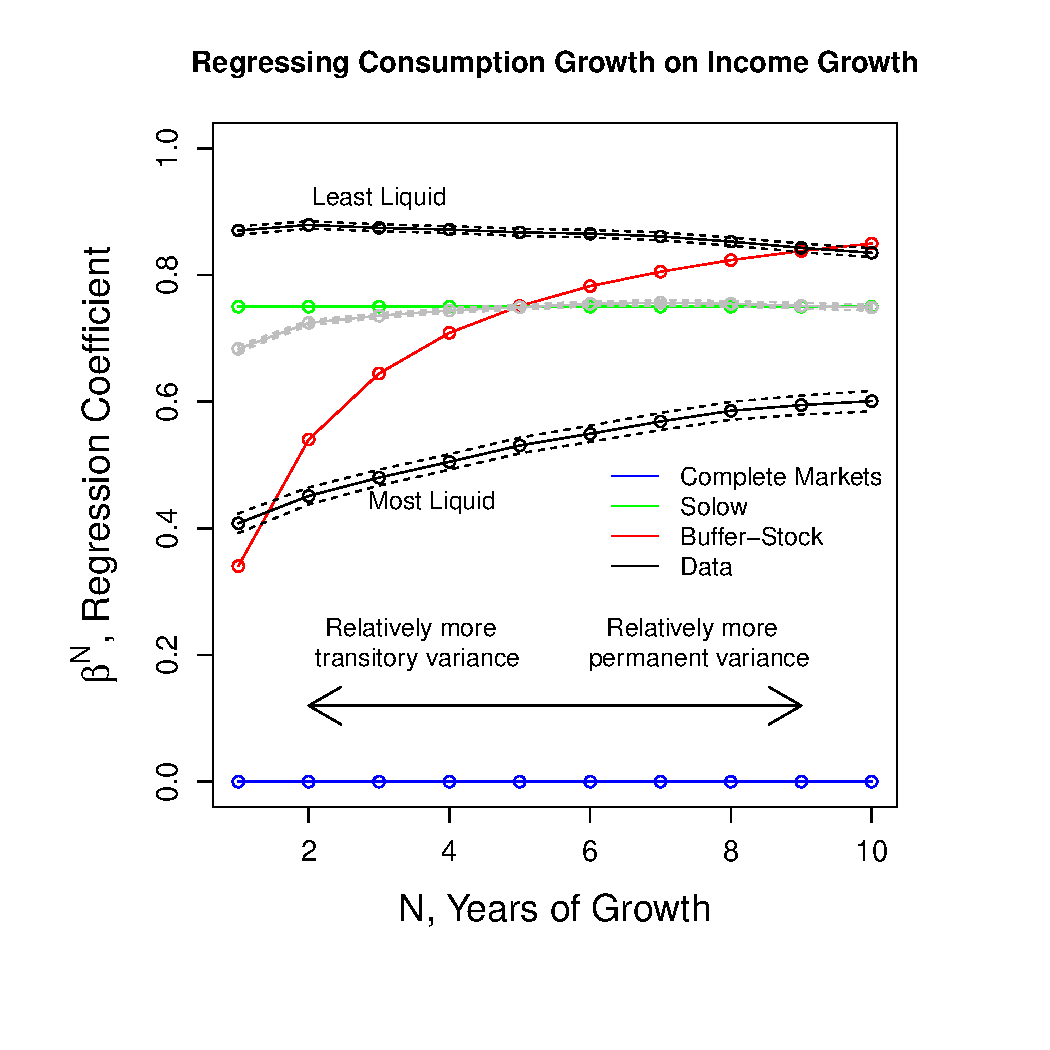
\includegraphics[scale=0.7]{\econtexRoot/Figures/basic_regression_liquid_wealth_level_lincome_head.pdf}
		\caption{Regression coefficients of consumption growth on income growth}
		\label{fig:GrowthReg}
	\end{centering}
\end{figure}

The gray line, along with 95\% confidence intervals, shows the results of these regressions using all households in the Danish sample. It is striking that the data appears to be closest to the Solow model, with only a small decrease in the regression coefficient over short periods. However, aggregating all households in this way hides a large degree of heterogeneity, particularly across households with different levels of liquid wealth. The two black lines show the regression coefficients where the sample is restricted to households in the lowest and highest quintiles of liquid wealth (averaged over the observed period) respectively. For households in the lowest quintile there is no evidence of consumption smoothing. As the regression coefficient is relatively stable for this group over N, the result that the marginal propensity to consume out of both transitory and permanent shocks are similar and very high is robust to a large degree of model misspecification, as discussed in the next section. Households in the top quintile of liquid wealth show a clear upward slope in figure \ref{fig:GrowthReg}, indicating a substantial degree of consumption smoothing. The fact that the regression coefficient for this group appears to asymptote well below 1 also suggests, in contrast to standard buffer-stock models, that the MPC out of permanent shocks for liquid households is significantly lower than 1.

\subsection{Aside: Why Not BPP? A Brief Introduction to the Time Aggregation Problem} \label{TimeAgg}
As explained above, our identification is going to come from the shape of income and consumption covariance over increasing periods of time. An obvious question is why we have chosen not to use the well known methodology of \cite{blundell_consumption_2008} who achieve identification of transitory shocks from the fact that a transitory shock in period $t$ will mean-revert in period $t+1$.\footnote{\cite{kaplan_how_2010} show in discrete time simulations that the methodology works reasonably well for standard calibrations of buffer-stock models and end up concluding ``The BPP insurance coefficients should become central in quantitative macroeconomics". However, some recent papers such as \cite{commault_how_2017} and \cite{hryshko_income_2018} have pointed to other potential problems of the methodology.} Unfortunately the method is not robust to the time aggregation problem of \cite{working_note_1960}. While macroeconomists have long been aware of the importance of time aggregation in time series regressions (see \cite{campbell_consumption_1989} for a well known example), the problem has been overlooked by the household finance and labor economics literature. We will therefore briefly describe the problem here. For a more detailed account with particular attention to BPP, see \cite{crawley_time_2018}.

Figure \ref{fig:TimeAgg} shows how the problem arises. The solid `Income flow' line shows the true income flow of a household who receives zero income throughout year 1, zero income for the first half of year two, and then a constant income flow of 1.0 per year during the second half of the second year and in the third year. The dashed line shows the observed \textit{total} income of the household in years 1, 2 and 3: zero in year 1, 0.5 in year 2 and 1.0 in year 3. The important thing to note is that despite there only being one `shock' to the income flow over the three year period, the na\"ive observer would assume there had been two shocks, one between years 1 and 2 and another between years 2 and 3. This effect is of particular importance to econometric techniques that make use of the auto-covariance structure of data processes. For example the first difference of a random walk in discrete time has no autocorrelation, but the first difference of a time-aggregated random walk in continuous time has an autocorrelation equal to 1/4. BPP uses time aggregated income data and achieves identification of transitory variance precisely though the auto-covariance structure. This is why the problem is particularly pervasive for this methodology: in a simulated dataset where households follow the permanent income hypothesis, that is they respond one-for-one to shocks to permanent income but not at all to transitory income shocks, the estimate for the consumption response to transitory income shocks using the BPP methodology is \textit{negative} 0.6.\footnote{This is for a simulation in which permanent and transitory shock variances are equal and shocks are uniformly distributed over the year.} 
	\begin{figure} 
	\begin{centering}
		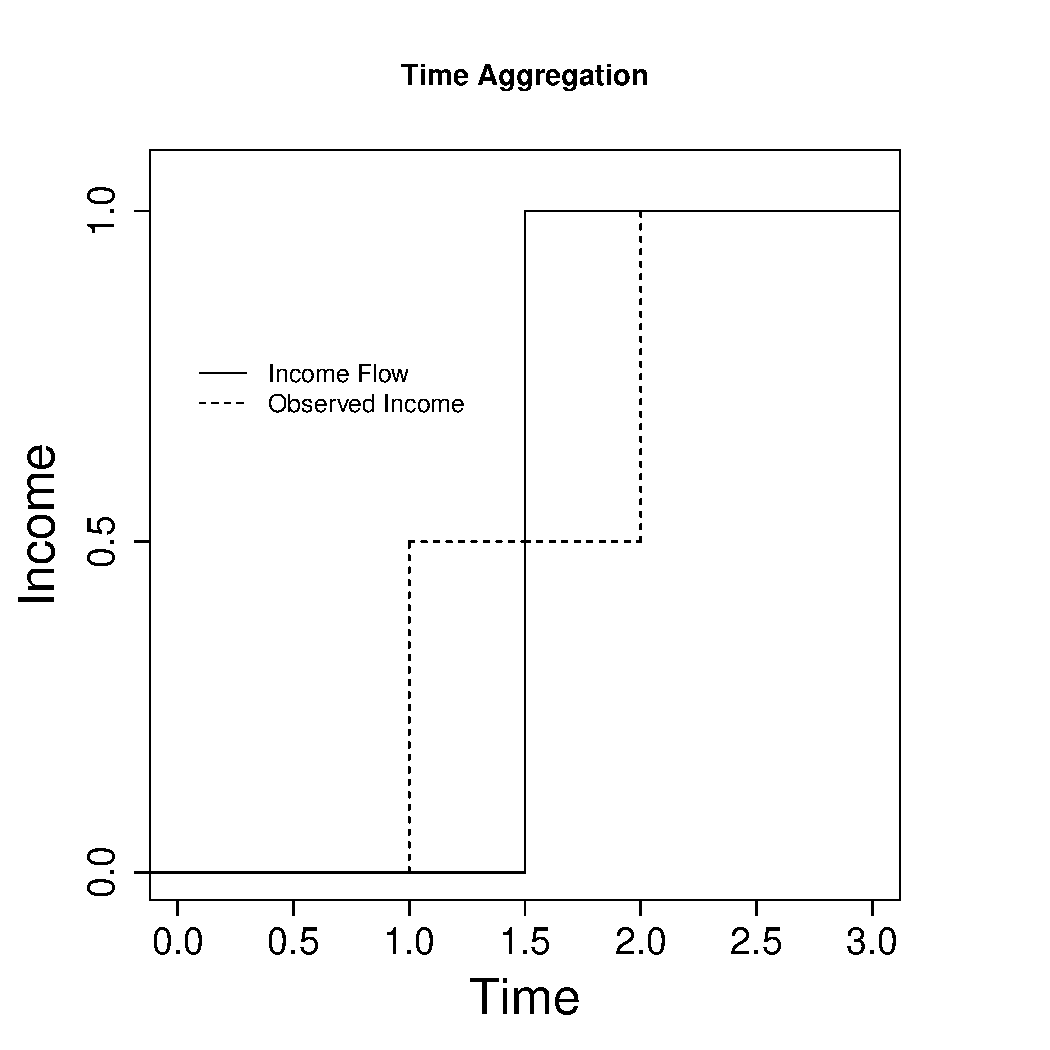
\includegraphics[scale=0.5]{\econtexRoot/Figures/TimeAggExample2.pdf} 
		\caption{The Time Aggregation Problem}
		\label{fig:TimeAgg}
	\end{centering}
\end{figure}

While it would be possible to stick very closely to the original BPP model and adjust the covariance restrictions to take account of the time aggregation problem,\footnote{\cite{crawley_time_2018} takes this more straightforward approach using the same PSID data as used in BPP.} we have found that in practice the underlying assumptions made by BPP (in particular that consumption follows a random walk) do not fit with the data.\footnote{\cite{kaplan_how_2010} show that without time aggregation, the BPP method correctly identifies the transitory consumption response in the period of the income shock regardless of the consumption dynamics going forward. This fact is again not robust to the time aggregation problem. With time aggregation taken into account the estimates are highly sensitive to assumptions about short term consumption dynamics.} Therefore we have chosen to attain identification in a manner similar to \cite{carroll_nature_1997} which allows us to be agnostic about the exact short term dynamics of income and consumption.

\subsection{Covariance Restrictions} \label{cov_restrictions}

\subsubsection{Income Dynamics: \cite{carroll_nature_1997}}
Our identification of permanent and transitory income variance will follow the methodology of \cite{carroll_nature_1997} closely. Our method will correctly account for time aggregation, but due to identification coming from income growth over 3, 4 and 5 years, rather than the covariance of income growth at time $t+1$ with time $t$ as in BPP, time aggregation only introduces a small bias in the estimates of \cite{carroll_nature_1997}. We will first describe the method without time aggregation and then show how the estimates need to be adjusted.

\cite{carroll_nature_1997} assume that income is composed of a permanent component that follows a random walk and a transitory MA(2) component. That is:
	\begin{align*}
	y_t &= p_t + \varepsilon_t + \theta_1 \varepsilon_{t-1} + \theta_2 \varepsilon_{t-2} \\
	p_t &= p_{t-1} +\zeta_t\\
	\end{align*}
where $\zeta_t$ and $\varepsilon_t$ are mean zero random variables, independent of each other and of themselves over time. Each has constant variance, $\sigma_{\zeta}$ and $\sigma_{\varepsilon}$ respectively. For $N \geq 3$ we have:
\begin{align}
\Delta^N y_t &= \zeta_t + \zeta_{t-1} + ... + \zeta_{t-N+1} \nonumber \\
& \qquad \qquad + \varepsilon_t + \theta_1 \varepsilon_{t-1} + \theta_2 \varepsilon_{t-2} - (\varepsilon_{t-N} + \theta_1 \varepsilon_{t-1-N} + \theta_2 \varepsilon_{t-2-N}) \nonumber \\ 
\Rightarrow \mathrm{Var}(\Delta^N y_t) &= N \sigma_{\zeta} + 2\underbrace{(1+\theta_1^2 + \theta_2^2)\sigma_{\varepsilon}}_\text{``Total'' transitory variance} \qquad \text{ for $N \geq 3$} \label{CS_identification}
\end{align}
Equation \ref{CS_identification} shows that the variance of income growth grows linearly with the number of years of growth beyond 3. The transitory component adds variance at the beginning and end of the growth period, but any transitory shock to income that occurs in the middle of the period does not affect income growth as it will have died out by the end. \cite{carroll_nature_1997} use this to identify the variance of permanent shocks, $\sigma_{\zeta}$, and the ``total'' transitory variance, $(1+\theta_1^2 + \theta_2^2)\sigma_{\varepsilon}$. While similar to BPP it is important to note that BPP attempts to identify the variance of initial impact of the transitory shock, $\mathrm{Var}(\varepsilon)$, rather than the ``total'' transitory variance. While the notion of ``total'' transitory variance will carry over naturally into the time aggregated case, the variance of the initial impact does not have a natural interpretation.

The administrative data we use in this paper is at an annual frequency and measures the sum of income over the observed year. If shocks to income occurred only on 1st January every year then we could use equation \ref{CS_identification} to identify permanent and transitory variance. It is important to distinguish between a model in which shocks happen about once a year (for example) but can occur at any point in the year, versus a model in which shocks to income happen on a timetable. The former can be modeled in continuous time with jumps occurring as a Poisson process approximately once a year. The later is best modeled as a discrete time model. In this paper we will take the former approach. While some types of jobs may have a regular schedule on which pay appraisals take place, many of the larger permanent shocks to income occur when a worker changes job which can occur at any point in the year. {\cite{low_wage_2010} show a significant portion of permanent income variance is explained by job mobility.} We (along with the literature) lack a clear understanding of what makes up the bulk of the transitory shocks to income and the Danish data is a potentially rich source for further research in this area.\footnote{While we use annual income data in this paper in order to match with our expenditure data, monthly labor income data is collected, along with employer-employee matching.} Furthermore, even if each individual household experienced shocks on a pre-set timetable, if the timetable itself varies across the year for different households, our approach would yield unbiased results. While there is a big change in going from an underlying annual process to a quarterly process, the further change from quarterly to continuous time is much smaller.\footnote{See \cite{crawley_time_2018}.} As the exposition is much simpler in continuous time, we will therefore choose to present our own method in continuous time.

To write the equivalent model in continuous time we define two underlying martingale processes (possibly with jumps), $P_t$ and $Q_t$ where $P_t$ will represent the \textit{flow} of permanent income at time $t$ and the change in $Q_t$ provides the transitory \textit{impulses} that generate the transitory income. We assume that for all  $s_1>s_2>s_3>s_4>0$:
\begin{align*}
\mathrm{Var}(P_{s_1}-P_{s_2})=(s_1-s_2)\sigma_P^2 \\
\mathrm{Cov}(P_{s_1}-P_{s_2},P_{s_3}-P_{s_4}) = 0 \\
P_s = 0 \qquad \text{if } s<0
\end{align*}
and similarly for $Q_t$. That is these martingales have independent increments. As a useful benchmark, two Brownian motions satisfy these criteria.

The natural generalization of the MA(2) transitory income process from \cite{carroll_nature_1997} is to allow for a generically shaped transitory income shock that decays to zero in under 2 years.\footnote{Previous studies have found little evidence of transitory dynamics lasting more that one year, but to be conservative and in line with BPP we allow transitory income to persist for up to two years.} Figure \ref{fig:GenericTransitory} shows an example of such a transitory income shape $f(t)$, but the model also allows for completely transitory shocks in which case $f(t)$ would be a delta function with all the income from the transitory shocks arriving as a mass at the time of the shock. In this model the \textit{flow} of income arriving at time $t$ is given by the flow of permanent income and the sum of income arising from any transitory shocks to income that have occurred in the previous two years:
\begin{figure} 
	\begin{centering}
		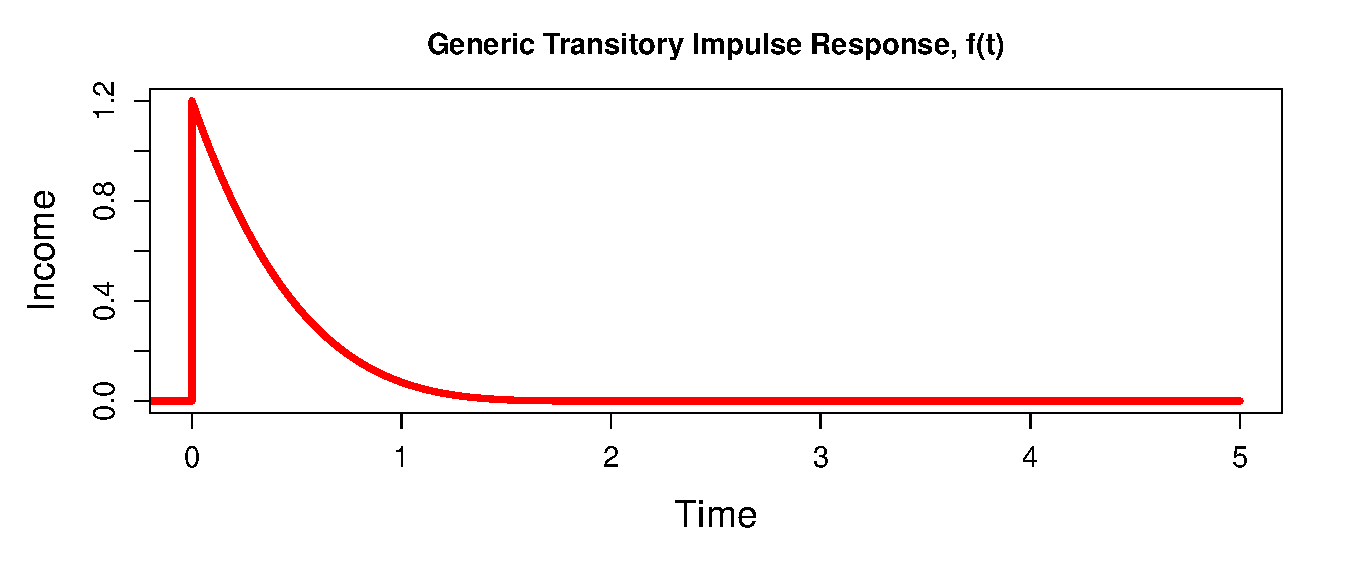
\includegraphics[scale=0.7]{\econtexRoot/Figures/GenericTransitory.pdf} 
		\caption{Generic Transitory Shock Impulse Response}
		\label{fig:GenericTransitory}
	\end{centering}
\end{figure}
\begin{align*}
y_t &= P_t + \int_{t-2}^{t} f(t-s)dQ_s
\end{align*}
We do not observe $y_t$ directly but instead $\bar{y}_T$, the time aggregated income over each one year period.
\begin{align}
\bar{y}_T = \int_{T-1}^{T} y_t dt \text{   for } T \in \{1,2,3...\}\label{income_TA}
\end{align}
Taking the $N^{th}$ difference for $N \geq 3$ we get:
\begin{align}
\Delta^N \bar{y}_T &= \int_{T-1}^{T} y_t dt  - \int_{T-N-1}^{T-N} y_t dt  \nonumber \\ 
&= \int_{T-1}^{T} (T-s)dP_s  + (P_{T-1} - P_{T-N}) + \int_{T-N-1}^{T-N} (s-(T-2))dP_s \nonumber \\
& \qquad + \Big(\int_{T-1}^{T} \int_{t-2}^{t} f(t-s)dQ_t dt -\int_{T-N-1}^{T-N}\int_{t-2}^{t} f(t-s) dQ_t dt \Big) \label{deltaNy}
\end{align}
The variance of time aggregated income of an $N$ year period is therefore:\footnote{See appendix \ref{sec:Identification} for full details of this derivation, including how we can approximate a log income process  with levels.}
\begin{align}
\mathrm{Var}(\Delta^N \bar{y}_T) &= (N-\frac{1}{3})\sigma^2_P +  2 \mathrm{Var}(\tilde{y}) \text{   for }n \geq 3 \label{variance}
\end{align}
This is similar to the non time aggregated case (equation \ref{CS_identification}) except the coefficient on permanent variance is $N-\frac{1}{3}$. This error, though having less serious consequences than for BPP, has nevertheless been overlooked by the large literature that studies income dynamics using panel data.\footnote{For examples see \cite{moffitt_trends_2012}, \cite{meghir_income_2004}, \cite{nielsen_impact_2004}, \cite{heathcote_unequal_2010} and more recent quantile regression approaches such as \cite{arellano_earnings_2017}.} As with the MA(2) case the transitory variance identified is the variance of ``total'' transitory income received in the year, $\tilde{y}$, where this is defined as:
\begin{align}
\tilde{y_T} = \int_{T-1}^{T}\int_{t-2}^{t} f(t-s)dQ_s dt \label{tot_income}
\end{align}
We will use equation \ref{variance} with $N \in \{3,4,5\}$.

\subsubsection{Consumption Dynamics}
Our approach will be to extend the identification of income variance by using growth over 3, 4 and 5 years to also identify the covariance of income and consumption. In contrast to BPP, which assumes consumption follows a random walk, we will instead assume that the impulse response to a transitory shock follows a generic path, $g(t)$, that like the transitory income shock has fallen to zero two years after the news of the shock. Figure \ref{fig:GenericTransitoryBPP} shows possible paths for both income and consumption, along with the alternative random walk impulse response of BPP. The best evidence for the speed at which the consumption response decays comes from \cite{gelman_what_2016} and \cite{fagereng_mpc_2016}, both of which show the response has entirely or almost entirely decayed two years after the shock. In section \ref{Consumption_persistence} we will show how this assumption may potentially bias the transitory consumption response up but that this bias is small, especially for all but the most liquid households. We will maintain the assumption from BPP that the consumption response to a permanent shock to income follows a random walk proportional to the permanent shock. Under these assumptions the instantaneous flow of consumption is given by:	\begin{figure} 
	\begin{centering}
		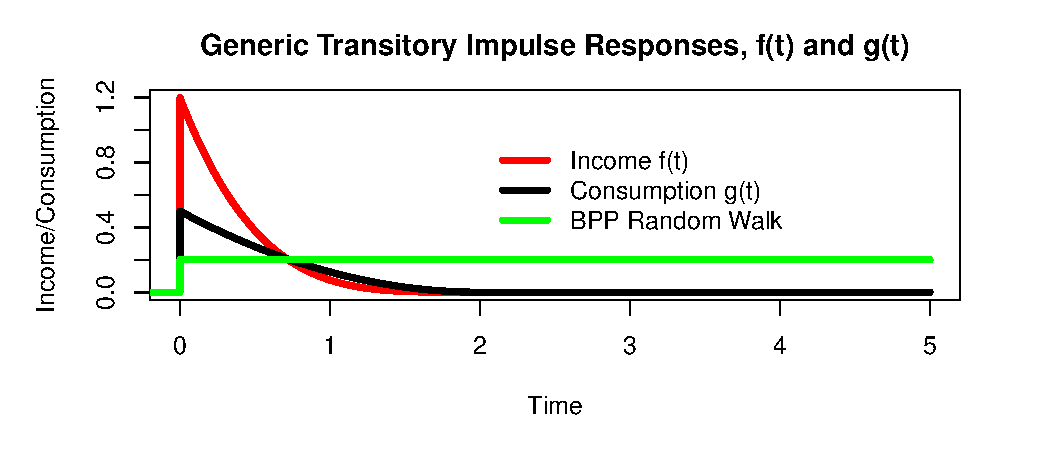
\includegraphics[scale=0.6]{\econtexRoot/Figures/GenericTransitoryConsumptionWithBPP.pdf} 
		\caption{Generic Transitory Shock Impulse Response}
		\label{fig:GenericTransitoryBPP}
	\end{centering}
\end{figure}
\begin{align*}
c_t  &= \phi P_s  + \int_{t-2}^{t} g(t-s)dQ_s  \\
\end{align*}
and the covariance of time aggregated income and consumption growth over $N \geq 3$ years is given by
\begin{align}
\mathrm{Cov}(\Delta^N \bar{c_T},\Delta^N \bar{y_T} ) &= \phi (N-\frac{1}{3}) \sigma^2_p + 2 \mathrm{Cov}(\tilde{c},\tilde{y}) \text{  for  } N\geq 3 \label{covariance}
\end{align}
where total transitory income, $\tilde{y}$ is given by equation \ref{tot_income} and total transitory consumption, $\tilde{c}$, is defined by:
\begin{align}
\tilde{c_T} = \int_{T-1}^{T}\int_{t-2}^{t} g(t-s)dQ_s dt \label{tot_cons}
\end{align}
Using the equations for variance (\ref{variance}) and covariance (\ref{covariance}) of income and consumption growth over $N$ years for at least 2 different values of $N$, we are able to identify the 4 unknowns we are interested in:
	\begin{itemize}
	\item[1.] $\sigma^2_p$ Variance of permanent shocks
	\item[2.] $\sigma^2_{\tilde{q}} = \mathrm{Var}(\tilde{y})$ Variance of transitory income received in a year
	\item[3.] $\phi$ Marginal Propensity to eXpend (MPX) w.r.t permanent income
	\item[4.] $\psi = \frac{\mathrm{Cov}(\tilde{c},\tilde{y})}{\mathrm{Var}(\tilde{y})}$ Regression coefficient of transitory consumption w.r.t transitory income over a year (MPX out of transitory income)
\end{itemize}
Our panel data covers 13 years and we choose to use growth over 3, 4 and 5 years to balance greater identification (longer growth periods give more power) with three identification problems that grow with $N$. The first is the fact that many households drop out of the sample if we demand they have reliable data for too many consecutive years. The second is that if the permanent shock in fact decays slowly over time (e.g. is in fact AR(1)), the bias this introduces will be larger for large $N$. Finally, the validity of running the regressions in levels (rather than logs) is reduced over large $N$ when the potential for the variance of income to change significantly from the start to end of the sample is high. In section \ref{threats_to_identification} and appendix \ref{robustness} we test the importance of these issues.

We follow BPP and use diagonally weighted minimum distance estimation, although our results are not significantly changed by using other popular weighting methods.\footnote{In general our results may be subject to misspecification problems, but the sample size of our data means that standard errors are small.}

As a lot of our analysis will focus on the parameter $\psi$ is it worth describing exactly what this is and why we have labeled it the marginal propensity to expend out of transitory income. If we were able to exactly observe transitory income and consumption resulting from transitory income then $\psi$ would be the regression coefficient of this transitory consumption on transitory income. If transitory income shocks have no persistence this is approximately a six month MPX (on average the shock will happen six months into the year so that the regression will pick up the change in consumption in the following six months). If transitory income shocks have a little persistence (appendix \ref{sample_selection} shows evidence of a small amount of transitory income persistence) $\psi$ can only loosely be interpreted as the MPX to an income shock and the reader should bear in mind that the true interpretation is, ``if income is higher by one unit this year due to transitory factors, then consumption this year will be expected to be higher by $\psi$ units".

\section{Data}
Our panel data on income and expenditure comes from Danish registry data from 2003-2015. This data has a number of advantages over survey based measures. First, the sample contains millions of households rather than thousands. Second, households are required by law to report their data so there is much less risk of selection bias through drop outs. Third, measurement error in income data is largely eradicated, as employees' income data is third party reported by their employer, compared to survey data where self reported income has been shown to be particularly unreliable for irregular income.\footnote{See \cite{david_income_nodate} for a survey of income measurement error issues in survey data.}

\subsection{Income} \label{income}
We are interested in income and consumption decisions at the household level. We define a household as having either one or two adult members. Two adults are considered to be in the same household if they are living together and a) are married to each other or have entered into a registered partnership, b) have at least one common child registered in the Civil Registration System or, c) are of opposite sex and have an age difference of 15 years or less, are not closely related and live in a household with no other adults.\footnote{Adults living at the same address but not meeting one of the three criteria are regarded as separate families. Children living with their parents are regarded as members of their parents' family if they are under 25 years old, have never been married or entered into a registered partnership and do not themselves have children. A family meeting these criteria can consist of only two generations. If three or more generations live at the same address, the two younger generations are considered one family, while the members of the eldest generation constitute a separate family.} In the panel data, an individual's household will change if he or she gets married or divorced. This leads to some selection bias given that we require households to survive for at least 5 years. Following the literature our baseline results will be reported using the labor income of the head of household.\footnote{See \cite{moffitt_income_2018} for an overview of the literature on income volatility in the PSID. In contrast to the PSID literature we define the head of household as the highest earner over the 13 year period in our sample. We believe this definition better fits the social structure in Denmark.} We will use after tax and transfer income as we are interested in the consumption response to these changes in income, although the method could be used to measure the extent of consumption insurance provided by the tax and transfer system. Our data comes from the administrative records from the tax authority. The tax reporting system in Denmark is highly automated and individuals bear little of the reporting burden. For employees income is reported by their employers and is thought to be highly accurate. The underground economy in Denmark is small. We remove business owners from the sample as their income may be less accurately reported, but more importantly, because the expenditure imputation method does not work well for them (see section \ref{cons_imputation}).



We work with the residual of income after controlling for observable characteristics of households that may affect their income and consumption. To start we remove households in the top and bottom 1\% of the income distribution. We then normalize by average household income over the observed period, and regress income on dummys for age, year, highest level of education, marital status, homeowner status and number of children along with interaction of age with education, marital status and homeowner status. We take the change in the residuals of this regression to be the unexpected income change for a household from one year to the next and remove households in the top and bottom 1\% of the unexpected income \textit{change} distribution.

\subsection{Imputed Expenditure} \label{cons_imputation}
Our expenditure data comes from imputing expenditure from income and wealth. Along with other Scandinavian countries, Denmark is unusual in that tax reporting includes information about wealth along with income, a legacy from the wealth tax that was phased out between 1989 and 1997. Following the methodology from \cite{browning_imputing_2003} and \cite{fagereng_imputing_2015} we impute expenditure using the identity:
\begin{align*}
\bar{C_t} \equiv \bar{Y_t} - \bar{S_t} = \bar{Y_t} - P_t - \Delta NW_t 
\end{align*}
where $\bar{C_t}$, $\bar{Y_t}$ and $\bar{S_t}$  are the sum of expenditure, income and savings over the year $t$ respectively. $P_t$ is contributions to privately administered pension schemes, for which we have very accurate data due to tax deductibility, $\Delta NW_t$ is the change in (non-pension, non-housing) net worth measured at the end of years $t$ and $t-1$. Banks and brokers are required to report the value of their clients' accounts on 31\textsuperscript{st} December each year, and the the tax reporting year runs from 1\textsuperscript{st} January to 31\textsuperscript{st} December, so the data for income and wealth reported in the tax returns matches with that required to use this identity to impute consumption. 

The method works well for households with simple financial lives. One of the biggest problems with the method is its inability to handle capital gains well. The income used in the imputation includes all labor income and capital income, however it excludes capital gains. The value of assets will vary both due to savings from reported income but also due to capital gains and losses. We handle this in a number of ways. First, we completely exclude housing wealth from our measures of net worth and saving, treating housing as an off balance sheet asset. The problem with treating housing in this way is that we must exclude households in years in which they are involved in a housing transaction. For the self employed, it is also difficult to distinguish between expenditure and investment in their business, so we exclude all households who receive more than a trivial amount of their income from business ventures. Finally, households that hold significant equity investments are likely to see sizable capital gains and losses. We make a naive adjustment by making the assumption that they hold a diversified index of stocks. While this will likely lead to significant measurement error for these individuals, the concern is mitigated first by the fact that stock holding is much more unusual in Denmark than in the US for example. Only around 10\% of households hold any stocks, and for many of those stocks make up only a small proportion of their total wealth. Furthermore, as we will explain in section \ref{Measurement_error}, measurement error in consumption is not a concern unless it is correlated with changes in income. This seems unlikely to be the case, except for households that hold significant equity in the firms in which they work. Another concern with the imputation method is transfers of wealth, say between family members or friends. Indeed imputed expenditure is negative for approximately 3\% of households and this may explain a proportion of that. We throw out both income and expenditure data for households in years in which their expenditure is negative. In appendix \ref{robustness} we test the robustness of our results to sample selection bias problems that these issues may give rise to.

As with income, we work with the residual of expenditure after normalizing by mean household income and controlling for the same observable features as income. We follow exactly the same steps as described in section \ref{income}.

In evaluating how much we can learn from such a measure, it should be compared to the best alternatives available to economists. In the original BPP paper the authors only have access to food expenditures from the PSID data and impute total non-durable consumption by comparison with the Consumer Expenditure Survey. Self reported consumption is also notoriously poor quality even in comparison to self reported income. Furthermore, in the PSID data the questions regarding food expenditure are ambiguous as to which period exactly the question is referring to. A recent paper by \cite{abildgren_consistency_2018} shows that the mean levels of expenditure from this imputation method are close to those from the national accounts (see figure \ref{fig:ConsumptionMeasures}). They find relatively large differences at the household level between the consumer survey and imputed expenditure although it is not clear that this is a problem with the imputation method as opposed to the survey measure. Indeed for car purchases, for which highly accurate register data are available, the consumer survey shows significant underreporting, consistent with \cite{koijen_judging_2014} who find 30\% underreporting of car purchases in the Swedish consumer survey. We believe that, with the exception of transaction level data reported by financial aggregation applications, the imputation method we use is some of the highest quality expenditure data available to researches for the types of questions we are addressing.
\begin{figure} 
	\begin{centering}
		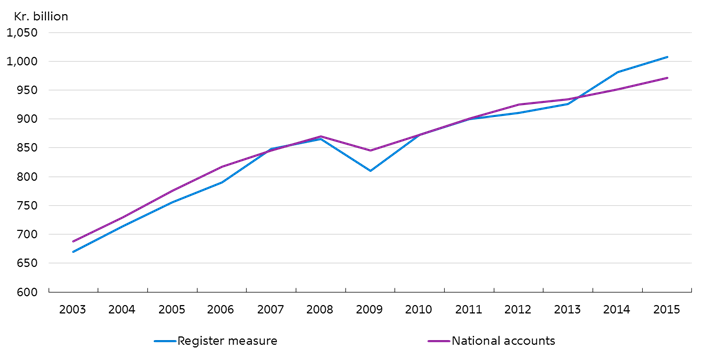
\includegraphics[scale=0.6]{\econtexRoot/Figures/consumption_measures.png} 
		\caption{Imputed Register Measure and National Account Measure of Expenditure (from \cite{abildgren_consistency_2018})}
		\label{fig:ConsumptionMeasures}
	\end{centering}
\end{figure}

\subsection{Sample Selection}
As our methodology requires income uncertainty to be relatively constant through the observed period\footnote{Appendix \ref{sample_selection} shows the assumption holds for this age group.} and the young and old are likely to have significant predictable income trends unobservable to the econometrician, we limit the sample to households headed by an individual between the age of 30 and 55 in 2008. Our final sample contains 7.7 million observations over 2004-2015 from an age group population total of 18.1 million. The selection criteria that reduces the sample size the most is the requirement that a household does not make a housing transaction for a period of 5 years. Table \ref{table:SummaryStatistics} shows summary statistics for all Danish households whose head fits into this age group as a whole as well as the sample we use in estimation. It is reassuring that both the mean and median values for after tax income and consumption are similar in the estimation sample and the population. Our estimation sample has much lower standard deviations as a mechanical result of excluding the top and bottom 1\% of the income and consumption distributions which contains extreme values. Sample selection shows up in homeownership and car ownership as we exclude those households that buy a house at the end of a five year period but who otherwise would be counted as renters. This also results in our sample being on average one year older than the population. Unhedged Interest Rate Exposure (URE) and Net Nominal Position (NNP) will be discussed in section \ref{monetary_policy}, but again the significant differences here are due to the housing transaction criteria. 
\begin{center} 
	\label{table:SummaryStatistics}
	\input\econtexRoot/Tables/summary_statistics.tex 
	\captionof{table}{Summary Statistics}
\end{center}

\section{Income and Consumption Characteristics by Household Wealth}
Using our entire estimation sample we find a mean MPX out of transitory shocks of 0.50 and a mean MPX out of permanent shocks of 0.72. However, these averaged results hide a significant amount of heterogeneity. From the standpoint of consumption theory it is the ability of households to self-insure with their own wealth that most determines how much they smooth their consumption over shocks. We divide our estimation sample into quintiles according to both liquid wealth (which we define as bank deposits\footnote{The results are little changed using any other definition of liquid wealth as long as housing and debts are excluded. See appendix \ref{robustness}.}) and net wealth. In each case wealth is measured as the mean household wealth holdings over the entire sample period.
\begin{figure}
	\centering
	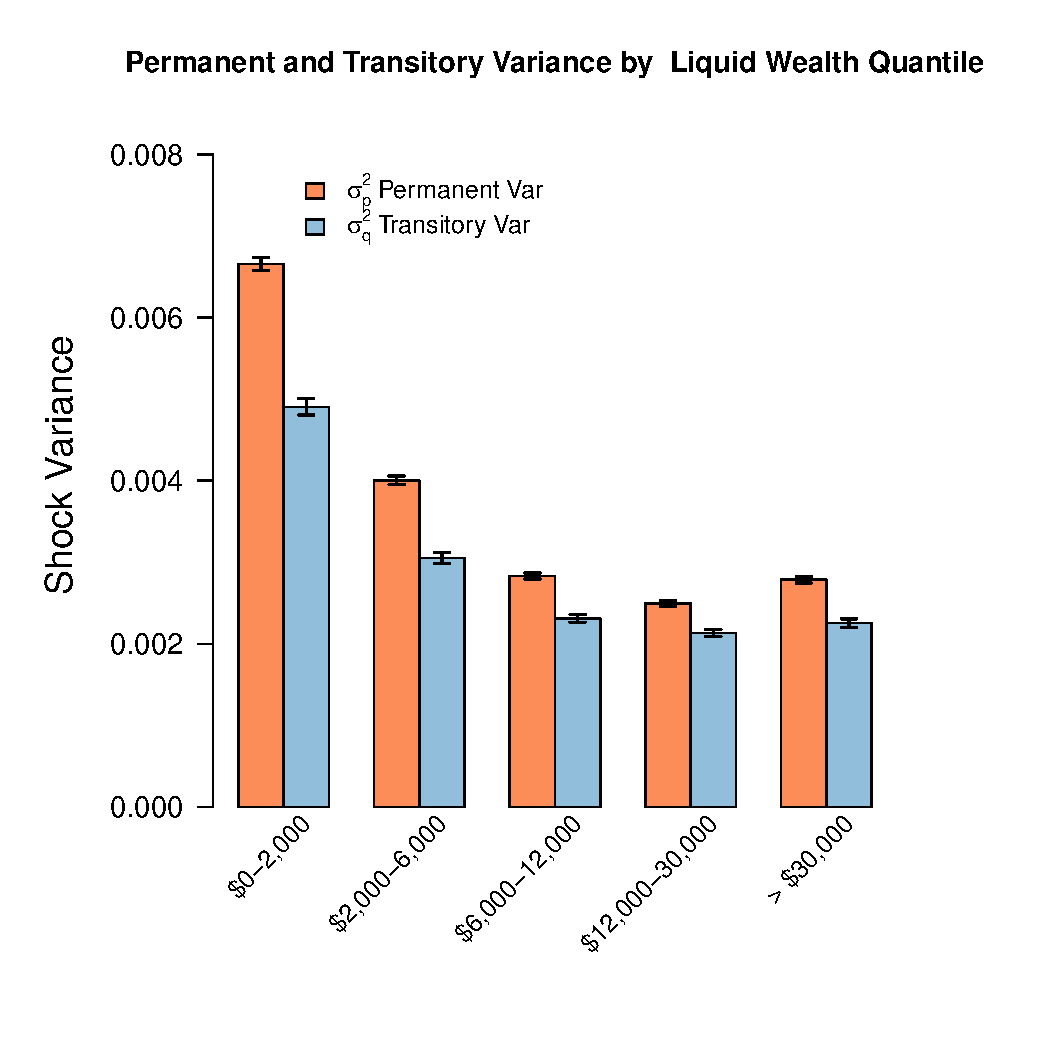
\includegraphics[scale=0.4]{\econtexRoot/Figures/VarianceByLiquidWealth_level_lincome_head.pdf}
	\centering
	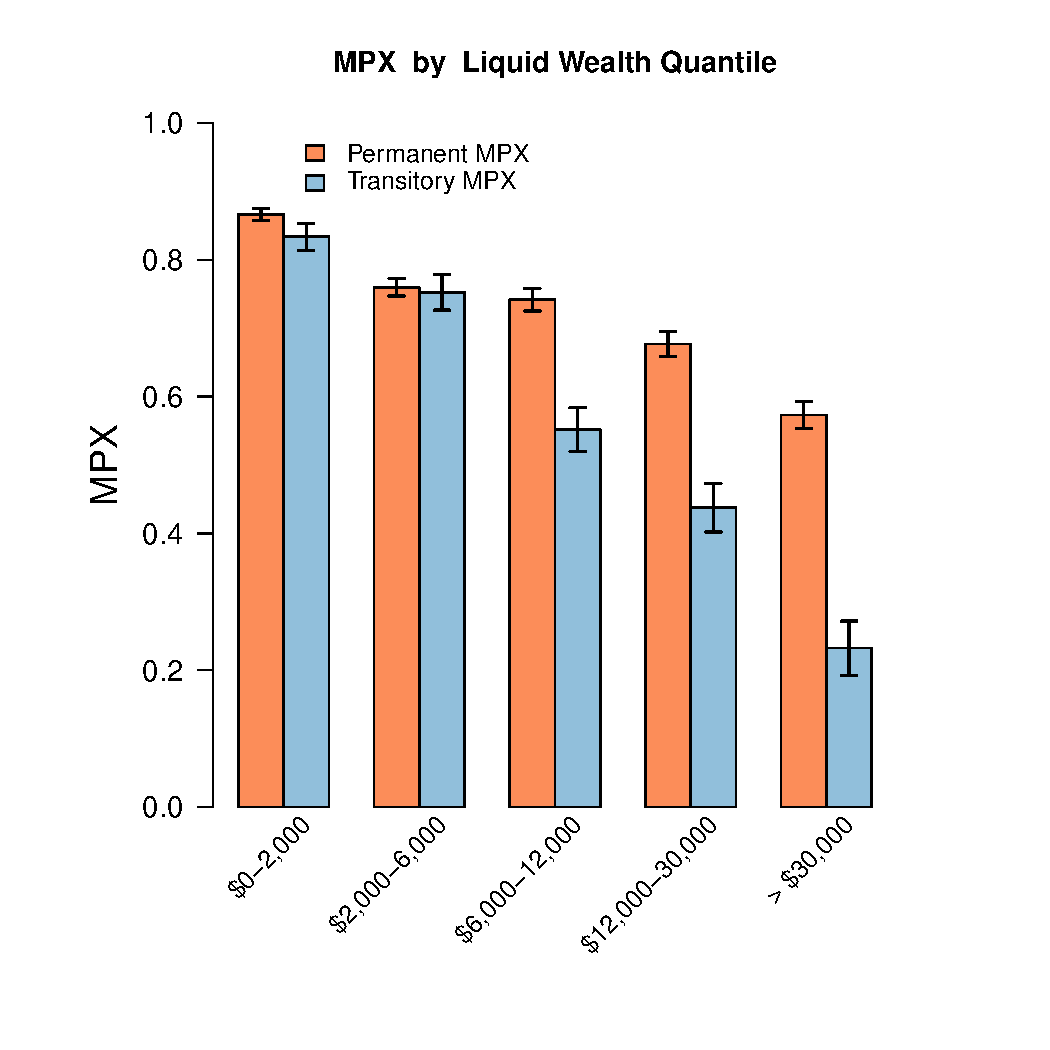
\includegraphics[scale=0.4]{\econtexRoot/Figures/MPXByLiquidWealth_level_lincome_head.pdf}
	\caption{Variance and MPX by Liquid Wealth Quintile}
	\label{fig:MPXByLiquidWealth}
\end{figure}

Figure \ref{fig:MPXByLiquidWealth} shows the estimated income variances and MPX's for households in each quintile of liquid wealth.\footnote{For these graphs, and all similar ones in this paper, the 95\% confidence intervals are shown above and below each quantile estimate.} Looking at the left hand variance panel first, it is noticeable that income uncertainty, and particularly permanent income uncertainty, is highest for households in the lowest quintile of liquid wealth. This is some evidence towards the idea that heterogeneous tastes (e.g. discount factors of risk aversion) may be more important that income risk in determining wealth held for precautionary saving. For households in the top three quintiles of liquid wealth it is remarkable how similar their level of income risk is. Note that in contrast to standard estimates of the US income process, permanent income variance in Denmark is slightly higher than transitory variance, likely due to the high levels of social insurance available in Denmark. The variance level, at just over 0.002 for these top three quintiles, represents a standard deviation of just below 5\% of permanent income per year.

Note that the estimates of income variance we obtain are highly sensitive to our treatment of outliers, but our MPX estimates do not change.\footnote{See appendix \ref{robustness} for evidence of this as well as a discussion of why this is the case.}

The right hand panel of figure \ref{fig:MPXByLiquidWealth} shows our estimates for the MPX out of permanent and transitory shocks by liquid wealth quintile. The lowest wealth quintile, who hold less than \$2,000 in bank deposits on average over the sample period, look somewhat like hand-to-mouth consumers. They respond almost equally to permanent and transitory shocks, spending over 80\% of income shocks in the year that it arrives. However, the fact that both permanent and transitory MPX's are very similar and significantly less than 1 suggests these households may be more accurately modeled as saving in an illiquid asset such as housing or a pension following a rule of thumb (say 20\% of income) and then living hand to mouth on the remainder. As the quintile of liquid wealth increases, the MPX out of both transitory and permanent income decreases. In the top quintile, formed of households that maintained a mean bank balance above \$30,000, the MPX out of permanent shocks is 0.57 and out of transitory shocks 0.23. From the point of view of theory the responsiveness of spending out of permanent shocks in this quintile is low, while that of transitory shocks is high. A more thorough discussion of how these results compare to a standard model calibrated to Danish characteristics will wait until section \ref{model}.
\begin{figure}
	\centering
	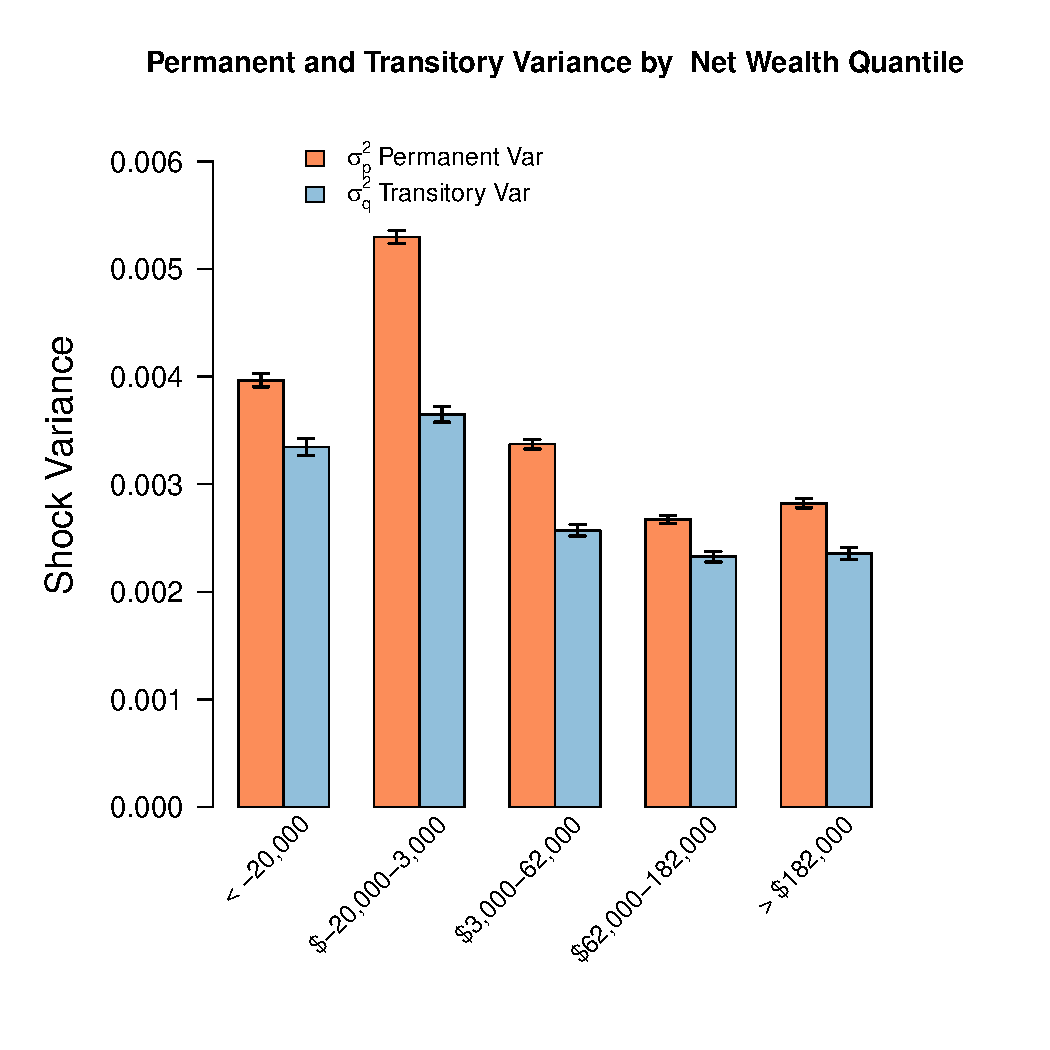
\includegraphics[scale=0.4]{\econtexRoot/Figures/VarianceByNetWealth_level_lincome_head.pdf}
	\centering
	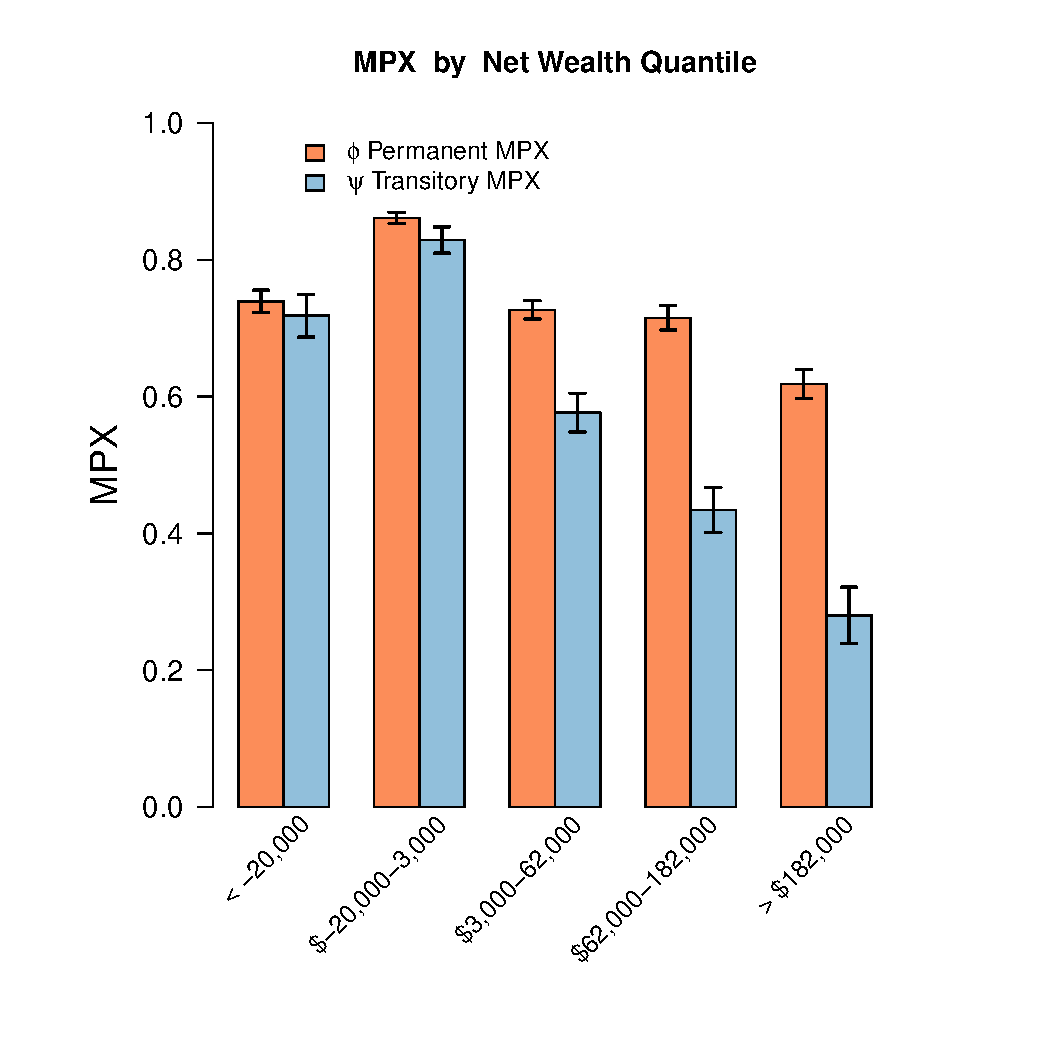
\includegraphics[scale=0.4]{\econtexRoot/Figures/MPXByNetWealth_level_lincome_head.pdf}
	\caption{Variance and MPX by Net Wealth Quintile}
	\label{fig:MPXByNetWealth}
\end{figure}

Figure \ref{fig:MPXByNetWealth} shows the estimates for households grouped by quintiles of net wealth. Here the pattern is slightly different. The quintile with the highest MPX out of both transitory and permanent income is the second lowest, the quintile that contains zero net worth. Households in the lowest quintile, those with over \$20,000 in net debt, do not seem to distinguish between permanent and transitory income shocks in their consumption responses, but their MPX for both is about 10 percentage points lower than the quintile with close to zero net wealth. The pattern for quintiles 3 to 5 looks similar to that for liquid wealth: the MPX out of transitory shocks falls sharply to around 0.28, while that out of permanent shocks also falls but more slowly to 0.62.

These results are broadly in line with the literature. The population mean of 0.5 for transitory MPX is a little higher than most estimates from table \ref{table:MPCLiterature}, but bearing in mind our estimate includes durables and is best compared to a six month MPC, it is certainly not an outlier. The MPX out of permanent shocks of 0.72 is also between the BPP estimate of 0.65\footnote{The permanent `insurance' coefficient estimated by BPP does not suffer as much from the time aggregation problem as the transitory coefficient.} and the estimate of 1.0 from \cite{gelman_response_2016}. The strength of the relationship between liquid wealth and MPC is similar to that found in \cite{gelman_what_2016} and stronger than in \cite{fagereng_mpc_2016}.

\section{Monetary Policy and the Redistribution Channel} \label{monetary_policy}
\cite{auclert_monetary_2017} lays out a clear and intuitive theory as to how heterogeneity in the marginal propensity to consume out of transitory shocks affects the transmission mechanism of monetary policy. He identifies five channels through which monetary policy can act, three of which are absent without heterogeneity. He then uses this theory to identify a small set of sufficient statistics that help distinguish which of these channels are of quantitative importance. While these statistics in theory are highly informative about the transmission mechanism of monetary policy, in his paper he has neither the data nor the methods to be able to estimate them convincingly. He states, ``As administrative quality household surveys become available and more sophisticated identification methods for MPCs arise, a priority for future work is to refine the estimates I provide here''. Given we have administrative data, along with a new method to estimate MPCs, a natural application of our work is to estimate Auclert's sufficient statistics. Our data has two significant advantages over previous efforts at this.\footnote{As well as \cite{auclert_monetary_2017}, a new version of \cite{fagereng_mpc_2016} also attempts to estimate these statistics.} First, our sample size is very large, containing a large percentage of all households in Denmark. Second, we have detailed balance sheet information for not only households within our sample, but also for those excluded from our sample. Furthermore, we are able to identify interest rate risk and nominal positions held by firms, foreigners and government so that the aggregate position is zero, as required in equilibrium. This allows us to avoid some of the more problematic assumptions used in aggregating household data.

\subsection{Distribution of MPX across NNP, URE and Income}
The redistribution effects of monetary policy depend crucially on two household characteristics, their Net Nominal Position and Unhedged Interest Rate Exposure.
\begin{itemize}
	\item \textbf{Net Nominal Position (NNP)} is the net value of a household's nominal assets and liabilities. It's relevance for analyzing the redistributive effects of monetary policy comes from the fact that an unexpected rise in the price level will decrease the wealth of households with positive nominal assets, redistributing it to those with negative NNP (who now have less real debt). In administrative data we are able to observe directly held nominal positions at the household level, including bank deposits and loans, bond holdings and mortgages. In aggregate the directly held NNP position of the household sector is negative, which from the national accounts we will see is balanced by the financial sector as well as foreigners.
	\item \textbf{Unhedged Interest Rate Exposure (URE)} measures the total amount that a household plans to save at the going interest rate that period. It is the difference between all maturing\footnote{We define 'maturing' assets and liabilites as those which are due to having their interest rates reset, also if they contractually exist for a longer period. For example, a 30 year variable rate mortgage with annual interest rate fixation periods is 'maturing' each year in our definition.} assets (including income) and liabilities (including planned consumption). For example, a household with a large variable rate mortgage will likely have very negative URE. For them the entire value of their mortgage will be adjusted to the new rate. When the interest rate rises for one period they will see their disposable income (after mortgage payments) go down, and hence if they have a high MPX their spending will also decrease. To calculate URE we assume all bank deposits and bank debt have a variable rate that changes instantaneously. For mortgage debt we directly observe the amount resetting over the following year. In Denmark reset of mortgages takes place on the first day in a quarter,\footnote{See appendix \ref{mortgage_market} for more details on the Danish mortgage market.} so we assume that the new rate will only apply for half the year. For all other assets and liabilities we assume a maturity of five years. As with NNP we find households on aggregate have a negative URE position in our data and this is counterbalanced by the interest rate position of the financial sector. See appendix \ref{URE_NNP_appendix} for more detail on how we calculate NNP and URE positions.
\end{itemize}

Figure \ref{fig:MPCAuclert} shows how the MPX varies across household values for URE, NNP and income. In each case the value on the x-axis has been divided by the mean level of expenditure of the entire sample. The top chart shows the estimated MPX for each decile of unhedged interest rate exposure. The deciles on the left contain households most negatively exposed to a rise in interest rates, those in the middle deciles have little exposure, while the two top deciles on the right have the most to gain from an interest rate rise. We have included in this chart data on both rates of homeownership and median liquid assets for each decile. A clear pattern emerges in which we can roughly categorize the deciles into three groups following \cite{violante_wealthy_2014}:
\begin{itemize}
	\item \textbf{Wealthy Hand-to-Mouth:} The first five deciles contain households with high levels of homeownership but relatively few liquid assets. These households have relatively high MPXs and it is likely their wealth is locked up in illiquid assets (mostly housing) and that they have large mortgages.
	\item \textbf{Poor Hand-to-Mouth:} The next three deciles tend to be renters with very little in the way of liquid assets either. These households have very high MPXs and are close to being truly hand-to-mouth. As they have few assets they have very little exposure to interest rates and cannot easily substitute consumption between periods, therefore their consumption behavior is likely not affected by changes in interest rates directly.\footnote{Neither the interest rate exposure channel nor the intertemporal substitution channel will have much impact on their consumption. Monetary policy will impact their expenditure strongly through income effects.}
	\item \textbf{Wealthy:} The top two deciles contain households who are both likely to be homeowners and hold very large liquid asset balances. These are likely households who own their house outright without a mortgage and have been able to build up a large stock of liquid assets. Relative to the other deciles they have low MPX and are likely able to use their assets to effectively consumption smooth.
\end{itemize}

The distribution of MPX with net nominal position follows a similar pattern. As mortgages in Denmark are a mixture of fixed and variable rates (see appendix \ref{mortgage_market} for details on the Danish mortgage market), we can think of a typical household with negative URE or NNP as having a large mortgage, while those with positive URE or NNP are wealthy households with lots of liquid wealth. This pattern has not been evident in previous attempts to measure the distribution of MPX across these dimensions. Most importantly for the theory, the average MPX for those with negative URE and NNP positions is significantly greater than those with positive URE or NNP. This confirms the intuition that households who owe a lot of floating rate debt have higher MPXs than those who own this debt, and leads to an interest rate exposure channel in which lowering interest rates increases expenditure. Note the mean levels of both URE and NNP are negative for the households in our estimation sample, so even a constant (positive) MPX would result in interest rate hikes reducing their expenditure if not balanced by indirectly held exposures.\footnote{In contrast, Auclert finds a mean positive URE across households. We believe the difference is partly due to the prevalence of fixed rate mortgages in the US, but also due to underreporting of expenditures, especially in the PSID data.}

The final chart in figure \ref{fig:MPCAuclert} shows the distribution of MPX with total household income. There is a clear downward trend. If the income of lower income households decreases more than that of high income households during a monetary policy contraction, then expenditure will go down by more than the mean income weighted MPX that would be the result of a representative agent model.

For comparison the distribution of  MPX out of permanent income shocks across these three dimensions can be found in appendix \ref{PermMPXbyURENNP}.
\begin{figure} 
\begin{centering}
	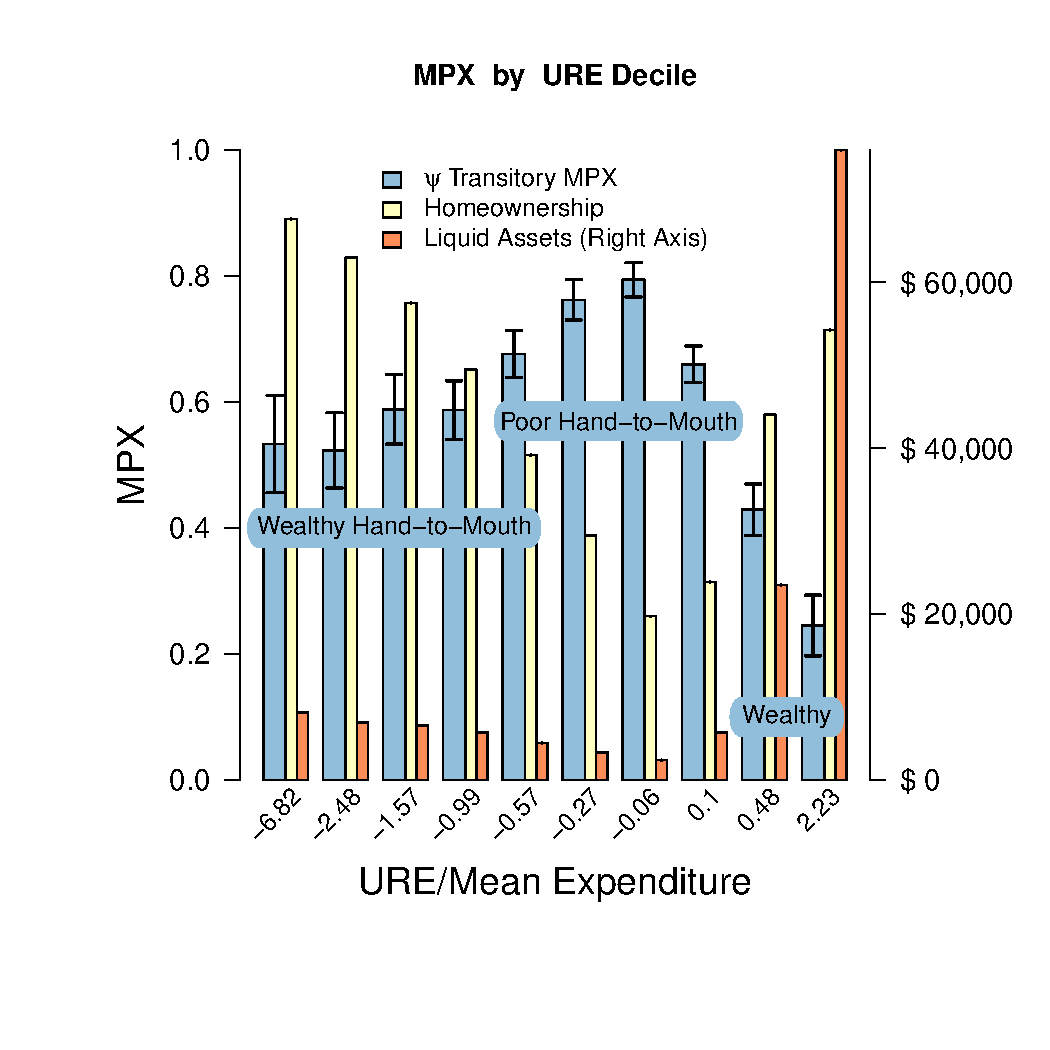
\includegraphics[scale=0.85]{\econtexRoot/Figures/MPXByUREdetailsPaper_level_lincome_head.pdf} \\
	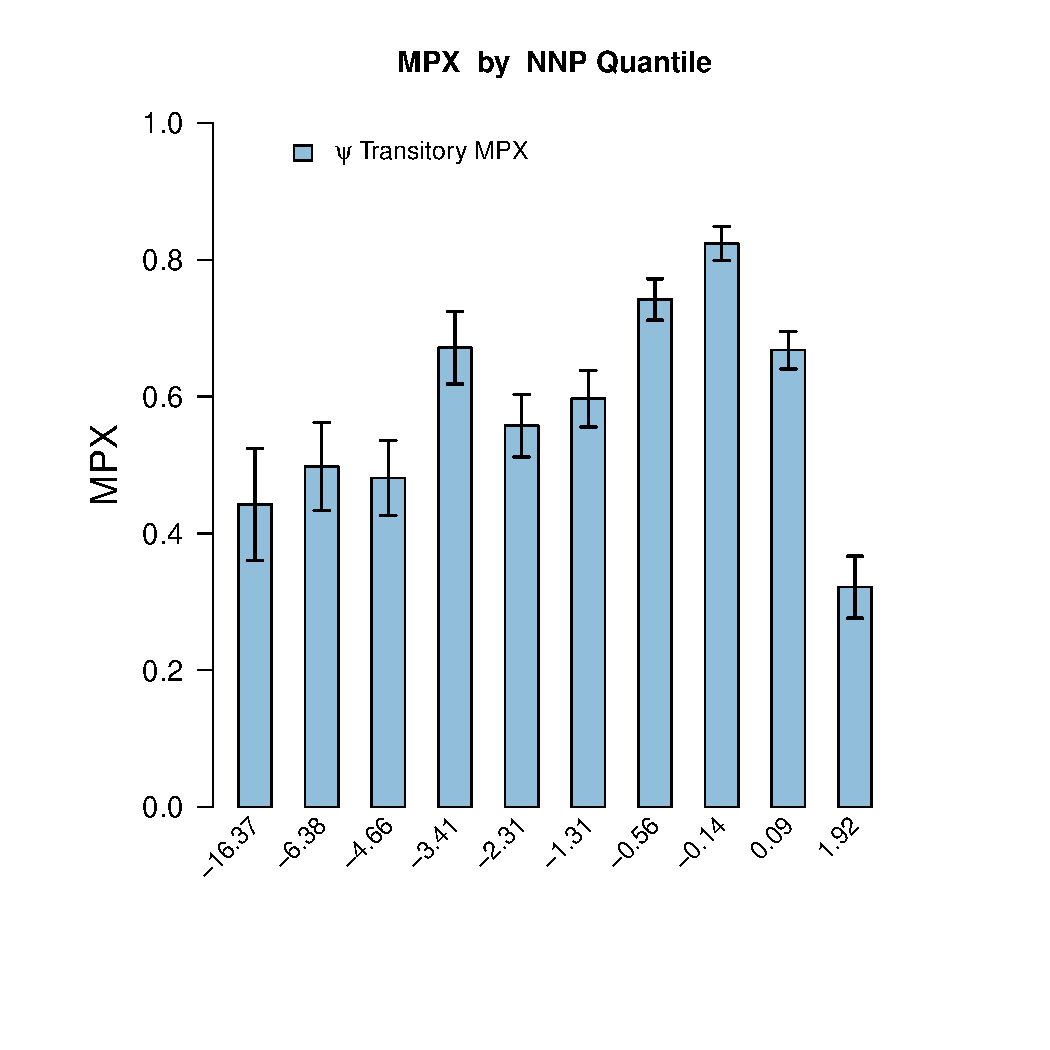
\includegraphics[scale=0.4]{\econtexRoot/Figures/MPXByNNP_level_lincome_head.pdf}
	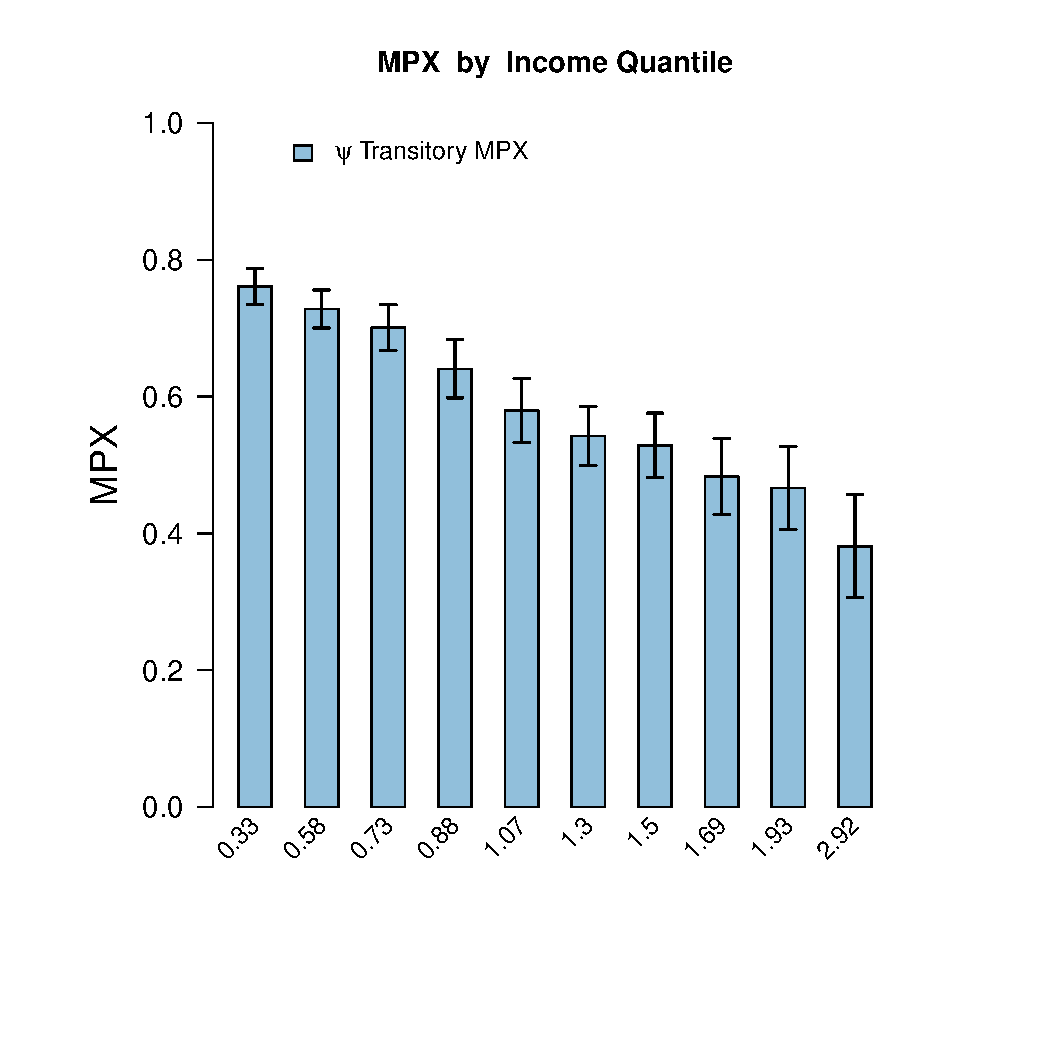
\includegraphics[scale=0.4]{\econtexRoot/Figures/MPXByIncome_level_lincome_head.pdf}
	\caption{MPX Distribution by URE, NNP and Income}
	\label{fig:MPCAuclert}
\end{centering}
\end{figure}

\subsection{Theoretical Setup and Sufficient Statistics}
Auclert's method is to consider individual households' consumption response to a monetary policy shock in which i) the real rate of interest changes for one period by $dR$, ii) the price level makes a one time change of $dP$ and then remains at the new level, and iii) aggregate income makes a transitory change of $dY$. While the dynamics here are clearly stylized, and in particular lack any lag in the economy's response, we believe such a simple experiment is highly informative as to the relative sizes of each transmission channel.

Auclert divides the effect of monetary policy on aggregate consumption into five distinct channels:
\begin{align} 
\frac{dC}{C} &= \overbrace{\mathcal{M}\frac{dY}{Y}}^{\text{Aggregate Income Channel}\qquad} \overbrace{ + \gamma \mathcal{E}_Y \frac{dY}{Y}}^{\text{Earnings Heterogeity Channel}\qquad} \overbrace{ - \mathcal{E}_P\frac{dP}{P}}^{\text{Fisher Channel}}  \nonumber \\
& \qquad \underbrace{ + \mathcal{E}_R \frac{dR}{R}}_{\text{Interest Rate Exposure Channel}\qquad}  \underbrace{ - \sigma \mathcal{S}\frac{dR}{R}}_{\text{Intertemporal Substitution Channel}} \label{auclert_channels}
\end{align}
where $\sigma$ is the elasticity of intertemporal substitution, $\gamma$ is the elasticity of relative income to aggregate income\footnote{Here we are making the simplifying assumptions that these quantities are common for all households, see \cite{auclert_monetary_2017} for a discussion.} and the five sufficient statistics, $\mathcal{M}$, $\mathcal{E}_Y$, $\mathcal{E}_P$, $\mathcal{E}_R$ and $\mathcal{S}$ are measurable in the data and defined in table \ref{table:auclertSS}. We choose to define these statistics to include the consumption effects coming from exposures not directly held by households. We allocate the aggregate URE and NNP exposure from our estimation sample into seven bins so that the total exposure across the economy is zero. These bins include households with (i) young (<30) and (ii) old (>55) heads, and exposures held by households indirectly through (iii) pensions funds, (iv) government, (v) non-financial corporates, (vi) financials and (vii) exposures held by the rest of the world. Within each of these bins we assume no heterogeneity so that the MPX with respect to these exposures is constant. This is a conservative assumption, likely to underestimate the size of the heterogeneous agent channels. Our assumptions on the level of these MPX's can be seen in table \ref{table:aggElas}.

We define $\mathcal{E}_R$ as:
\begin{align}
\mathcal{E}_R = \frac{1}{C}\Bigg[ \sum_{i \in \text{URE deciles} } \text{MPX}_i \text{URE}_i + \sum_{j \in \text{bins}} \text{MPX}_j \text{URE}_j \Bigg]
\end{align}
where $i$ sums over the ten deciles of URE, $j$ over the seven bins defined above and $C$ is aggregate household expenditure in the economy. This method of dealing with the fact that aggregate exposure does not equal zero in the estimation sample is different to the approach taken by Auclert. He assumes the residual exposure is distributed equally across households in the sample. By making use of the national accounts we believe we are able to get a better handle on the likely MPX's to attach to this residual exposure. Table \ref{table:auclertSS} shows the definitions we use for each of the five measurable statistics in equation \ref{auclert_channels}.

\begin{minipage}{1.0\textwidth}
	\begin{center}
		\captionof{table}{Sufficient Statistics Definitions}
		\label{table:auclertSS}
		\resizebox{\textwidth}{!}{\begin{tabular}{ccl}
			\textbf{Statistic} & \textbf{Definition} & \textbf{Description} \\
			\hline
			$\mathcal{M}$ & $\frac{1}{C}\Bigg[ \sum\limits_{i \in \text{Income deciles} } \text{MPX}_i Y_i + \sum\limits_{j \in \{\text{young,old}\}} \text{MPX}_j Y_j \Bigg]$ & Income-weighted MPX \\
			$\mathcal{E}_Y$ & $\mathcal{M} - \overline{\text{MPX}}\frac{Y}{C}$ & Redistribution elasticity for Y \\
			$\mathcal{E}_P$ & $\frac{1}{C}\Bigg[ \sum\limits_{i \in \text{NNP deciles} } \text{MPX}_i \text{NNP}_i + \sum\limits_{j \in \text{bins}} \text{MPX}_j \text{NNP}_j \Bigg]$ & Redistribution elasticity for P \\
			$\mathcal{E}_R$ & $\frac{1}{C}\Bigg[ \sum\limits_{i \in \text{URE deciles} } \text{MPX}_i \text{URE}_i + \sum\limits_{j \in \text{bins}} \text{MPX}_j \text{URE}_j \Bigg]$ & Redistribution elasticity for R \\
			$\mathcal{S}$ &$1-\frac{1}{C}\Bigg[ \sum\limits_{i \in \text{Consumption deciles} } \text{MPX}_i C_i + \sum\limits_{j \in \{\text{young,old}\}} \text{MPX}_j C_j \Bigg]$ & Hicksian scaling factor \\
			\hline
		\end{tabular}}
	\end{center}
	\tiny \textbf{Note: } $\overline{\text{MPX}}$ is the mean MPX over all households in the economy. $Y$ and $C$ are aggregate household income and consumption respectively. bins refers to the seven categories for which we have allocated URE and NNP exposures outside our estimation sample. \{young,old\} are the two bins that contain young and old households (the other five bins only relevant for URE and NNP exposures as $Y$ and $C$ measure \textit{household} income and consumption).
\end{minipage}

\subsection{Out of Sample MPX}
The assumptions we make about the MPX of the young and the old, as well as out of indirectly held URE and NNP exposures are shown in table \ref{table:aggElas}. In each case we believe we have made conservative choices that will underestimate the size of the interest rate exposure channel of monetary policy. For the young we choose an MPX of 0.5, in line with the rest of the population. As the young have aggregate negative exposures, choosing an MPX on the low side is conservative. Similarly for the old we choose an MPX of 0.5, on the high side for this age group. The assumption that there is no heterogeneity in MPX within these groups is also a very conservative assumption.

Much of the URE and NNP exposure is not held directly on the balance sheet of households, but instead indirectly through pension funds, corporates and the government. There is significant evidence that the MPX out of shocks to the value of pension wealth, stocks or the government balance sheet is substantially lower than the MPX from income. We choose to use the estimate from \cite{maggio_stock_2018} that households' MPX from changes in stock market wealth is about 10\%. This choice is the most quantitatively important as the bin containing the most exposure is the financial sector, which is positively exposed to interest rate increases. This may seem surprising as banks are typically thought of having long term assets and short term debt that would result in negative URE exposure. However, our findings are in line with \cite{landier_banks_2013} who find that the aggregate financial sector benefits from interest rate hikes, although there is a large amount of heterogeneity between different banks. An important caveat is due here: we focus on the MPX out of changes in the assets indirectly held by households through the financial sector and do not assume any spending or lending response at the bank level. While this may be a reasonable assumption in good times when banks are not credit constrained, it is especially not the case during a banking crisis. This could possibly result in monetary policy being much less effective during a banking crisis as the interest rate exposure channel to household spending is counterbalanced by a channel from bank balance sheet interest rate exposure to lending.\footnote{It should be noted that our analysis here is all on the household side. Evidence suggests firms are also sensitive to changes in cash flow, for example see \cite{blanchard_what_1994}.} 

We choose an MPX of zero for government and the rest of the world. There is no evidence that households respond in any significant way to changes in the government's balance sheet, and furthermore a low MPX is a conservative assumption for the size of the heterogeneous agent channels. As Denmark is a very small part of the world economy we assume foreigners spend a negligible proportion of their wealth there.
\begin{center}
	\label{table:aggElas}
	\input ./Tables/URE_NNP_table.tex
	\captionof{table}{Aggregating Redistribution Elasticities}
\end{center}

\subsection{Results}
Our estimates of the five sufficient statistics are shown in table \ref{table:suff_stats}. The aggregate income channel is summarized by $\mathcal{M}$ that we estimate to be 0.52. This means that if income for all households in the economy increased by 1\%, aggregate consumption would increase by 52 basis points. This is broadly in line with calibrations of saver-spender models designed to fit evidence from \cite{campbell_consumption_1989}. We find little role for the redistribution effect of income, $\mathcal{E}_Y$, despite the clear negative correlation between income and MPX seen in figure figure \ref{fig:MPCAuclert}. $\mathcal{S}$, the Hicksian scaling factor, is 0.49, which reduces the size of the intertemporal substitution channel by close to a half.

The two statistics of most interest are $\mathcal{E}_P$ and $\mathcal{E}_R$, both of which act through redistribution from households with low MPX to those with high MPX. $\mathcal{E}_P$ is estimated to be -0.75 suggesting that a one time increase in the price level of 1\% increases aggregate consumption by 75 basis points due to redistribution from those with large nominal assets to those with large nominal debts. This Fisher channel of monetary policy is emphasized in \cite{doepke_inflation_2006}. The interest rate exposure channel is also large. We estimate  $\mathcal{E}_R$ to be -0.26 suggesting that a 1\% increase in the interest rate decreases expenditure by 26 basis points.

For both of these channels, but particularly the interest rate exposure channel, it is informative to compare to the size of the intertemporal substitution channel. An increase in the real interest rate reduces aggregate consumption today by $\sigma \mathcal{S}$ multiplied by the percent change in the rate where $\sigma$ is the intertemporal elasticity of substitution. Reliable estimates of $\sigma$ have been elusive to the economics profession, but there is very little evidence of a large positive number. \cite{havranek_measuring_2015} provides a meta-study of the elasticity of intertemporal substitution and finds a mean of zero from studies using macro data, and 0.3-0.4 for those using micro data. Many of these micro studies suffer from identification problems.\footnote{See \cite{carroll_death_2001} for a critique of many older studies of the elasticity of intertemporal substitution.} A recent paper of \cite{best_estimating_2018} makes use of mortgage notches in the UK to overcome some of these problems. They estimate the average elasticity of intertemporal substitution to be 0.1, which would result in a size of the intertemporal substitution channel of monetary policy being 0.05, over five times smaller than our estimate of the interest rate exposure channel.\footnote{Our decomposition does not allow easy comparison of the interest rate exposure channel with the aggregate income channel, as we do not make assumptions about how much aggregate income changes. \cite{cloyne_monetary_2016} compare mortgagors with outright homeowners and find the aggregate income channel is larger than the direct effect of higher mortgage payments.}
\begin{center}
	\captionof{table}{Sufficient Statistics}
	\label{table:suff_stats}
	\input ./Tables/sufficient_stats.tex
\end{center}
A long outstanding question in monetary economics is why monetary policy acts with a lag. Two competing theories are habits models such as \cite{fuhrer_habit_2000} and sticky information models such as \cite{mankiw_sticky_2002}. A recent paper by \cite{carroll_sticky_2018} finds evidence towards the idea that households react fast to their own idiosyncratic income shocks but news about macroeconomic shocks takes time to be absorbed. A possible third alternative to both of these is that households respond strongly to their realized income today, but not to income anticipated in the future. As it takes time for variable rate mortgages to reset (typically 6 months to up to 5 years in Denmark), this would result in the interest rate exposure channel acting with a delay. Indeed the literature on consumption responses to transitory income shocks has generally found little difference between anticipated and unanticipated responses. Many of the estimates in table \ref{table:MPCLiterature} use anticipated shocks (such as tax rebates) as an instrument and find large MPCs, suggesting households do not necessarily pay attention to anticipated cash flows until they arrive. A recent paper by \cite{ganong_consumer_2017} shows this very clearly: there is a sharp consumption drop in the month that unemployment benefits expire, an entirely anticipated event. A model which takes these results seriously, along with a large role for the interest rate exposure channel of monetary policy, could be a fruitful area of future research. 

\section{Benchmark Model and Taste Shock Extension} \label{model}
In this section we calibrate a standard incomplete markets model to Danish characteristics, including the liquid wealth distribution in Denmark, and use it to see if we can match the consumption responses we measure in the data.\footnote{By calibrating to the liquid wealth distribution, we are implicitly assuming households cannot access any of their illiquid wealth. A model such as \cite{violante_wealthy_2014} or \cite{gorea_liquidity_2017} which allows households to buy and sell an illiquid asset at a cost would result in lower overall MPCs.}

Motivated by the fact that the standard model results in lower transitory MPX numbers than we find in the data, we make a simple extension to the model to account for potentially large preference shocks. We propose that such shocks, which have generally played a much smaller role in the literature than income shocks, are perhaps quantitatively more important for precautionary savings behavior.

\subsection{Benchmark Model Calibrated to Danish Data} \label{benchmark_model}
Our baseline model is the now very familiar buffer-stock saving model of \cite{carroll_buffer_1997}. Given market resources ($\boldmath{\mLevBF}_t$), households in this model maximize expected utility:
\begin{align*}
	\mathbb{E}_t \sum_{i=t}^{\infty} \beta^i u(\cLevBF_i)
\end{align*}
subject to the constraints:
\begin{align*}
	\aLevBF_t = \mLevBF_t - \cLevBF_t \\
	\bLevBF_t = R\aLevBF_t \\
	\yLevBF_t = \theta_t \pLevBF_t \\
	\pLevBF_t = \Psi_t \pLevBF_{t-1} \\
	\mLevBF_t = \bLevBF_t + \yLevBF_t
\end{align*}
Where the felicity function, $u(\cLevBF)$ is CRRA. We calibrate our model to match both the income uncertainty (as measured using our methodology) and the liquid wealth distribution in Denmark. To be able to match the liquid wealth distribution, especially at the low end, we follow \cite{krusell_income_1998} and \cite{carroll_distribution_2017} and allow for ex-ante heterogeneity in the discount factor $\beta$. Specifically an agent $i$ has a discount factor $\beta_i$ where $\beta_i$ is i.i.d across agents and follows a uniform distribution between $\beta_{low}$ and $\beta_{high}$. These two parameters allow us to match the fact that while the mean level of liquid assets is high, about half of all households have close to zero liquid assets. Matching the lower part of this distribution is critical to generate transitory consumption elasticities substantially above zero. The Lorenz curve for liquid assets, both in the data and in the model, is shown in figure \ref{fig:Lorenz}.\footnote{We calibrate to the 20th, 40th and 60th percentile of liquid wealth, leaving out the 80th percentile. This is to better match the wealth of the lower half of the distribution, which is necessary to achieve reasonably high MPCs in a model like this. The figure shows that the fit in the upper half of the distribution is less precise.}
\begin{figure} 
		\centering
		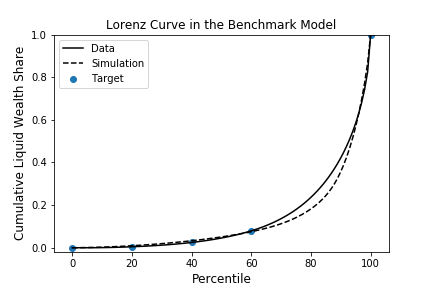
\includegraphics[scale=0.45]{\econtexRoot/Figures/benchmark_Lorenz.png}
		\caption{Lorenz Curve for Danish Liquid Assets}
		\label{fig:Lorenz}
\end{figure}

\subsection{Model with Preference Shocks}
The baseline model exhibits two features in tension with the data. First, the marginal propensity to consume out of transitory income shocks, while exhibiting the right shape relative to the liquid wealth, is too low relative to the data. Second, as would be expected in a consumption smoothing model like this, the path of expenditure is significantly less volatile than income. This is strongly at odds with the data which show the standard deviation of changes in expenditure to be around 0.37, compared to 0.12 for income. There is very little evidence on the true size of expenditure shocks, partly because of large measurement errors known to be present in consumption survey data. While we believe the 0.37 number from our data also contains measurement error, as well as large expected expenditures such as new cars for which finance may be readily available, it seems likely that the expenditure shocks could be large. Indeed typical financial advice to maintain a buffer stock will mention unexpected costs such as medical bills or a leaky roof before income shocks.\footnote{For example Forbes magazine in 2016 suggests ``you could find yourself thrown off by a chipped tooth or fender bender. So having an emergency fund padded with nine months of the highest earner's net income may help give you a bit more peace of mind that you could weather a financial storm.''} A simple tweak to the baseline model can help the model fit the data along both these dimensions. To achieve this we add a preference shock to expected utility:
\begin{align*}
\mathbb{E}_t \sum_{i=t}^{\infty} \beta^i \mathcal{X}_i u(\cLevBF_i)
\end{align*}
where $\mathcal{X}_i$ is i.i.d. and calibrated such that the variance of consumption is large.\footnote{We choose preference shocks with an annual standard deviation of 0.3. While this seems large, the resulting consumption change standard deviation is 0.18, significantly lower than 0.37 that we observe in the data.}

\subsection{MPX by Liquid Wealth}
The top panel of figure \ref{fig:CSTW} shows how the transitory MPX of the two models compares with the data. While the fact that the MPX decreases with liquid wealth quintile is robust in both models and in the data, there are two features worth noting. 

First, large preference shocks are required to push the transitory MPX close to the levels we see in the data. Many recent papers, such as \cite{krueger_macroeconomics_2016}, have attempted to carefully quantify the macroeconomic dynamic consequences of a serious heterogeneous agent model, but thus far have not included significant preference shocks in their calibrations. The evidence here suggests that such shocks may have a quantitatively important role to play, especially in increasing the marginal propensity to consume. To the extent that the precautionary motive is driven by preference shocks as opposed to income shocks, social insurance for unemployment will not reduce precautionary savings as much as these models presently suggest.

Second, neither of the two models is able to explain the high MPX out of transitory shocks that we observe for the top quintile of liquid assets. These households, who hold a mean balance above \$30,000, appear very responsive to transitory shocks despite their large buffer stock they could potentially use to smooth income shocks.
\begin{figure} 
	\begin{centering}
		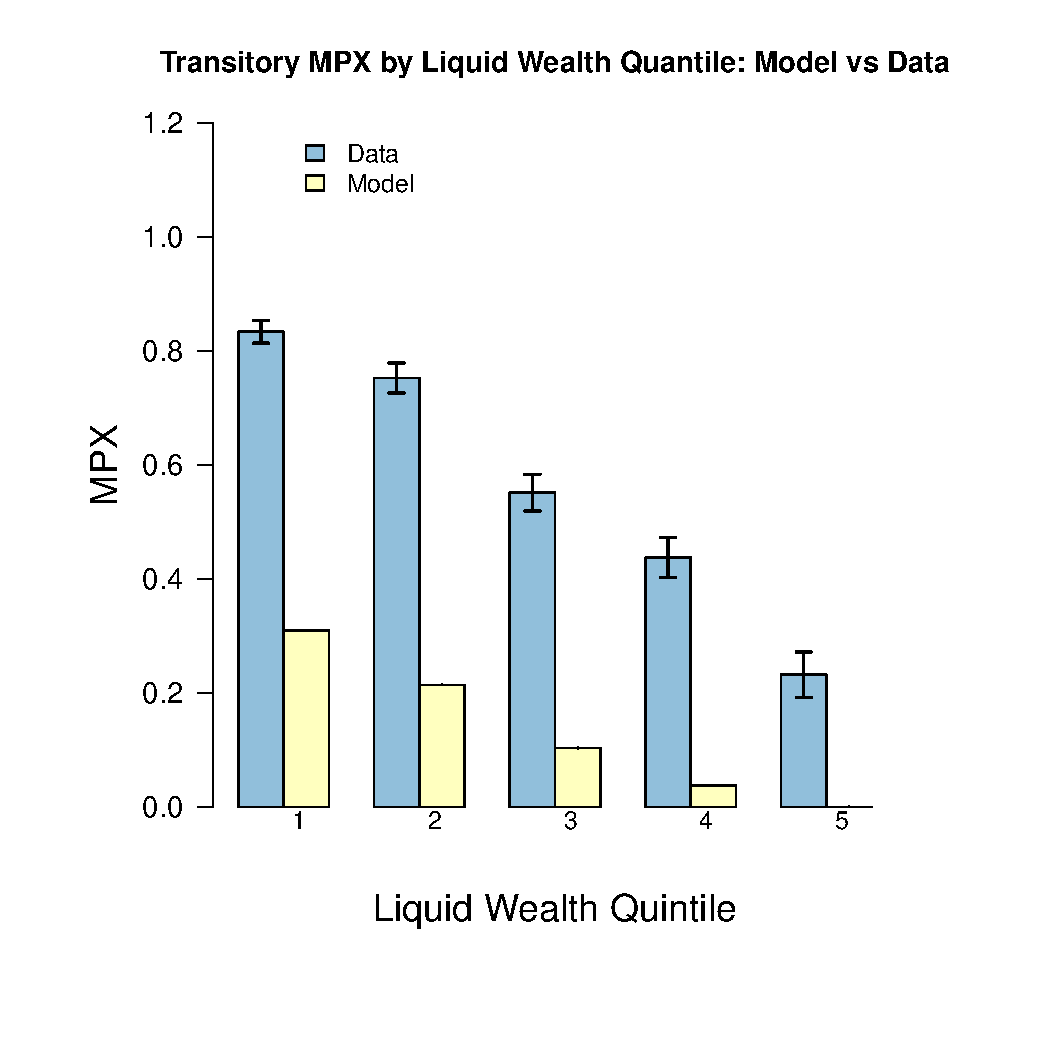
\includegraphics[scale=0.4]{\econtexRoot/Figures/CSTW_tran_denmark.pdf}
		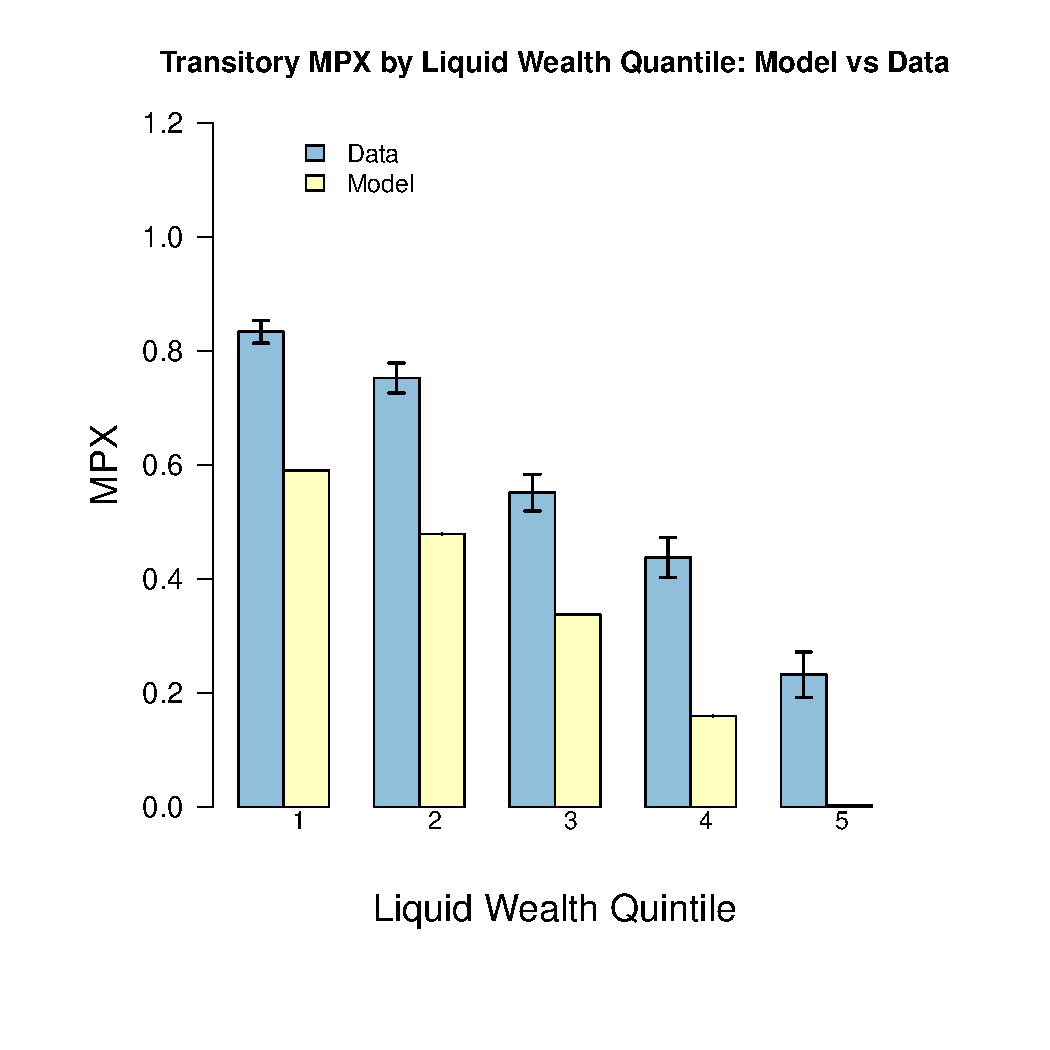
\includegraphics[scale=0.4]{\econtexRoot/Figures/CSTW_tran_denmark_pref.pdf}
		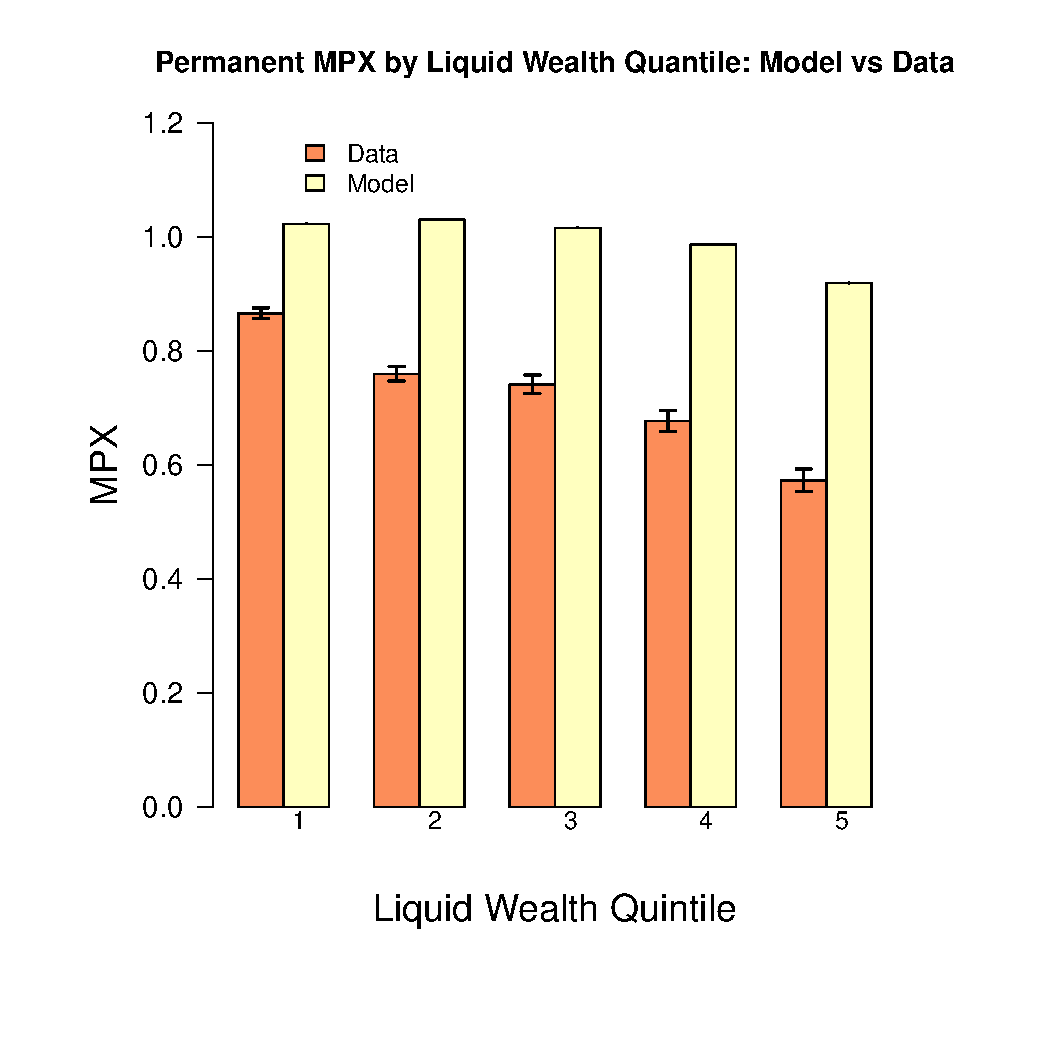
\includegraphics[scale=0.4]{\econtexRoot/Figures/CSTW_perm_denmark.pdf}
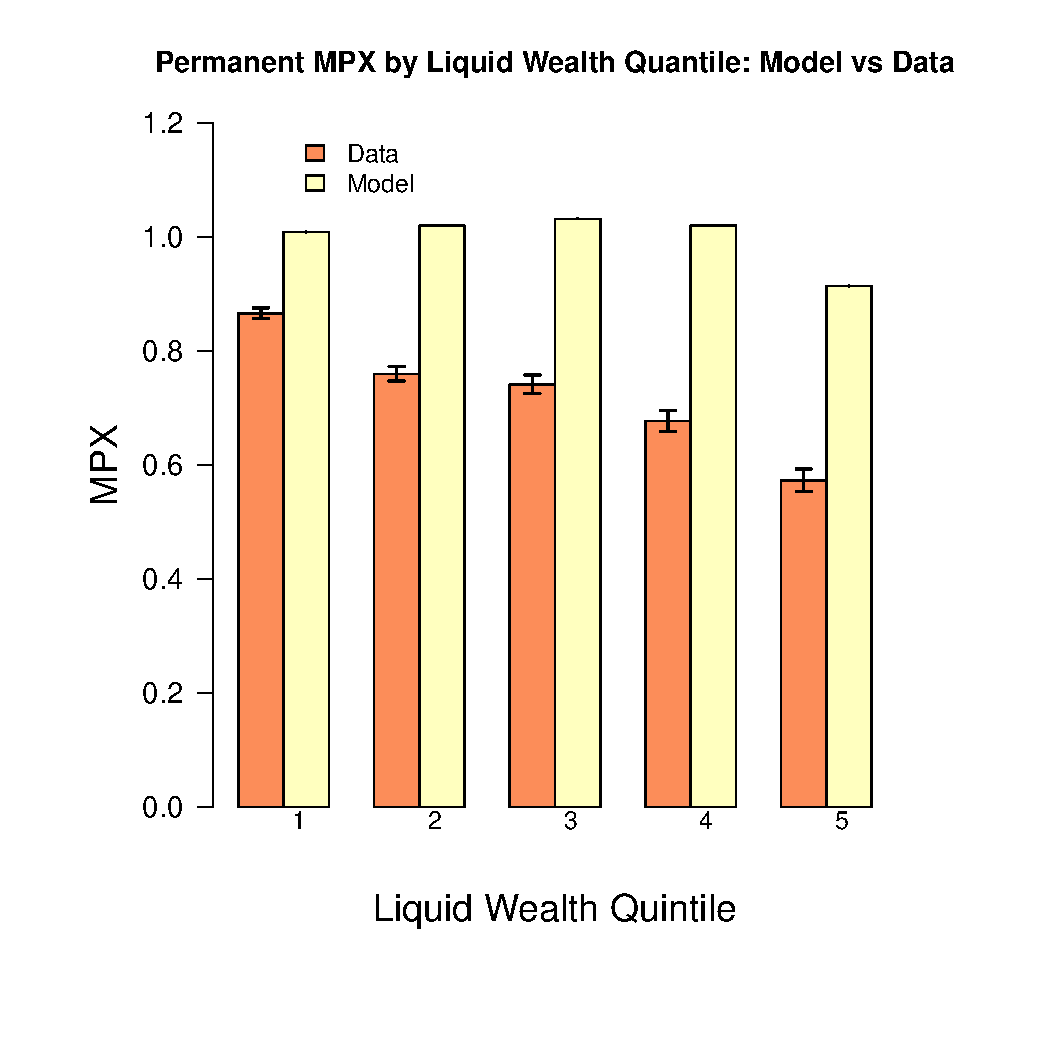
\includegraphics[scale=0.4]{\econtexRoot/Figures/CSTW_perm_denmark_pref.pdf}
		\caption{Baseline model (LHS) and Preference Shock Model (RHS) with the Data}
		\label{fig:CSTW}
	\end{centering}
\end{figure}

The bottom panel of figure \ref{fig:CSTW} shows another failure of both these two simple models: neither is able to capture the fact that the consumption response to permanent shocks is substantially below 1, even for middle and low quintiles of liquid wealth. \cite{straub_consumption_2018} shows that a lifecycle model with non-homothetic preferences may do better along this front.

\section{Threats to Identification}
\label{threats_to_identification}

\subsection{Durables} \label{durables}
A critique of our empirical methodology is that it does not take account of durable goods, while our data includes all spending (except on real estate) and therefore includes large and durable goods such as cars and home improvements. The empirical model assumes that in response to a transitive income shock, expenditure increases temporarily for up to two years. This is entirely consistent with a model that includes durable goods. However, the model assumes that in response to a permanent shock to income, expenditure increases once to a new permanent level. A model that included durable goods would instead imply a large one off expenditure on durable goods to get the household up to their desired stream of durable good services, followed by a decrease back to a permanent level of spending that accounts for replenishing the higher level of depreciating durable goods.

To make this idea more explicit, it will help to write down a simple model. The model will show that our empirical methodology continues to estimate the consumption response to permanent and transitory shocks, but that these need to be interpreted carefully. The model uses the same income process as section \ref{cov_restrictions}. Remembering the income process is made up of two martingale processes, $P_t$ and $Q_t$, which may have jumps, instantaneous income is given by:
\begin{align*}
dy_t = \Big( \int_{0}^{t}dP_s \Big) dt  +dQ_t 
\end{align*}
while instantaneous expenditure now has both a durable and non-durable component:
\begin{align*}
dc_t = \phi_{nd} \Big( \int_{0}^{t} dP_s  \Big) dt + \phi_{d} dP_t + \psi dQ_s
\end{align*}
Here we have assumed that the expenditure response to transitory shocks is instantaneous, but it would not change things to assume as before that the response decays to zero after two years. However, it is important that the durable component of the expenditure response to permanent shocks occurs instantaneously with the shock (or very soon after). Aggregating income and consumption annually gives:
\begin{align*}
\Delta^N \bar{y}_T &=  \Big(\int_{T-N-1}^{T-N} (s-(T-N-1))dP_s  + \int_{T-N}^{T-1}dP_s + \int_{T-1}^{T} (T-s)dP_s \Big) \\
& \qquad + \Big(\int_{T-1}^{T} dQ_t -\int_{T-N-1}^{T-N} dQ_t \Big) \\
\Delta^N \bar{c}_T &= \phi_{nd} \Big(\int_{T-N-1}^{T-N} (s-(T-N-1))dP_s  + \int_{T-N}^{T-1}dP_s + \int_{T-1}^{T} (T-s)dP_s \Big) \\
& \qquad + \phi_d \Big(\int_{T-1}^{T} dP_t -\int_{T-N-1}^{T-N} dP_t \Big) \\
& \qquad + \psi \Big(\int_{T-1}^{T} dQ_t -\int_{T-N-1}^{T-N} dQ_t \Big) \\
\end{align*}
From this we can calculate the covariance:
\begin{align*}
\mathrm{Cov}(\Delta^n \bar{c_T},\Delta^n \bar{y_T} ) &= \phi_{nd} \mathrm{Var}(\Delta^n \bar{y_T}) \\
& \qquad + \phi_d \Bigg( \int_{T-1}^{T} (T-s) \sigma_P^2 dt - \int_{T-N-1}^{T-N}(s-(T-N-1)) \sigma_P^2 dt \Bigg) \\
& \qquad + \psi\Bigg(\int_{T-1}^{T}  \sigma_Q^2 dt + \int_{T-N-1}^{T-N}\sigma_Q^2 dt\Bigg) \\
&= \phi_{nd} (n-\frac{1}{3})\sigma_P^2 + 0 +  2 \psi \sigma_Q^2
\end{align*}
So the durable component of the covariance cancels out and our identification method correctly identifies $\phi_{nd}$ and $\psi$, but is unable to identify $\phi_d$.

However, if there is some delay between the household receiving the permanent income shock and purchasing the durable goods, then this introduces an upward bias into the estimate of transitory MPX. The size of the bias grows with the number of months delay between the permanent income shock and the durable goods purchase, plateauing after twelve months at a level of $\frac{\sigma^2_p}{2\sigma^2_q}\phi_d$. Figure \ref{fig:durable_bias} shows how this bias increases with the delay.
\begin{figure} 
	\begin{centering}
		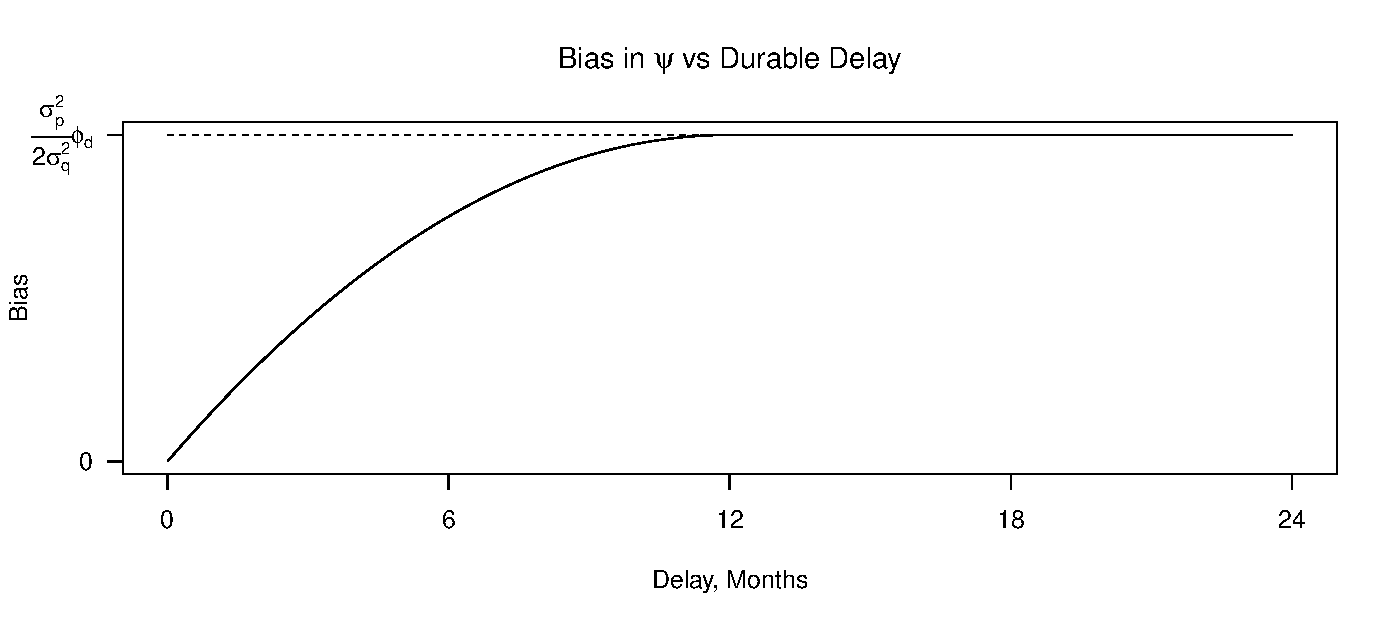
\includegraphics[scale=0.6]{\econtexRoot/Figures/DurableBias.pdf}
		\caption{Bias in Transitory MPX with Delay in Durable Goods Purchase}
		\label{fig:durable_bias}
	\end{centering}
\end{figure}

In order to quantify how large this bias may be in practice we make use of the car registry data available in Denmark. Using data on the current value of cars owned by a household, we perform the same residual calculation to find the change in car value that is unpredictable with the household characteristics we are able to observe. We then construct two new expenditure panels, one in which we remove expenditures on cars and a second in which we make a proxy for non-durable consumption by removing expenditures on cars multiplied by $\frac{1}{0.421}$ (Car purchases make up 42.1\% of durable expenditure in Denmark).
\begin{align*}
C_T^{\text{nocar}} = C_T - \Delta \text{CarValue} \\
C_T^{\text{nondurable}} = C_T - \frac{1}{0.421}\Delta \text{CarValue}
\end{align*}
The second, non-durable proxy consumption panel, can be modeled as the true non-durable consumption panel with classical measurement error added. This classical measurement error does not bias our estimates, so we can use this non-durable proxy panel to estimate an unbiased MPC out of transitory shocks, where the MPC does not include durable expenditures.
\begin{figure} 
	\begin{centering}
		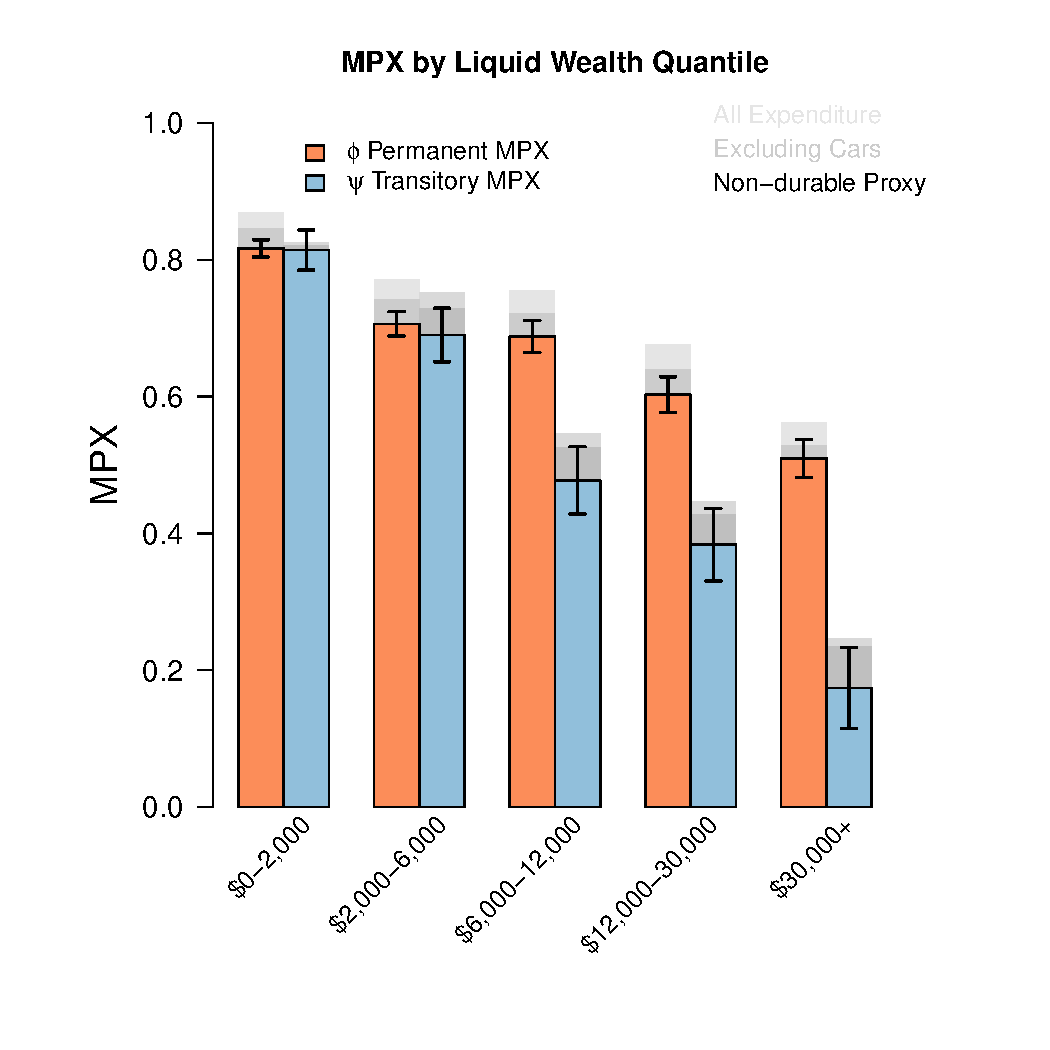
\includegraphics[scale=0.4]{\econtexRoot/Figures/MPXByDurables_nodurableproxy.pdf}
		\caption{MPX Removing Cars and Using the Non-durable Proxy Panel}
		\label{fig:MPXByDurables}
	\end{centering}
\end{figure}

The results of this exercise can be seen in figure \ref{fig:MPXByDurables}. Even without bias, we would expect the non-durable proxy estimates to be lower than those including all expenditures as the definition of transitory MPX changes over the three panels to exclude cars and then all durable goods. For the lower quintiles of liquid wealth it therefore looks as though the bias is likely very small, as non-durable goods make up 10\% of spending and the MPX estimates are smaller by an amount in this region. For the top quintile of liquid wealth there looks to be some bias, with the estimate of MPX for all expenditures decreasing from 25\% to an MPC for non-durable goods of 17\%.

While there is some evidence that our results may be biased up for those in the top quintiles of liquid assets, this bias will only have a small effect on our overall conclusions. As the relevant number for the monetary policy exercise is the MPX rather than the MPC, we have chosen not to adjust our baseline results using this method and accept that a small bias may exist in our data. It should be noted that such a bias will cause the heterogeneous channels of monetary policy to appear smaller than they actually are.

\subsection{Labor Elasticity} \label{labor_elasticity}
The empirical results of this paper estimate MPX to be at the high end of the literature. The results also conflict with standard consumption theory, particularly at the higher end of the liquid wealth distribution. It is possible that these high transitory MPX estimates are being driven by reverse causality: in years when households wish to spend more, they increase their labor supply. In this case our assumption that labor income is exogenous would be false. To get a sense of the quantitative magnitude of the bias such reverse causality could induce, in appendix \ref{labor_elasticity_model} we calibrate a model with both preference shocks and labor supply elasticity. We find the effect is quantitatively small, with both the true MPX and the estimates using our method being close to zero for a simulation of households with liquid wealth in the top quintile. However, for extreme values of preference shocks and labor elasticity, we can generate estimates of the transitory MPX to be as high as 0.25, when the true MPX is 0.08.\footnote{Estimates of the Frisch elasticity in micro-data studies range from 0 to 0.5, while macroeconomic studies generally find a much larger elasticity of between 2 and 4 (see \cite{peterman_reconciling_2016}.). We not consider estimates of the Frisch elasticity in the macroeconomic range as it seems likely to us that these estimates are high due to labor market frictions over the business cycle, rather than genuine labor supply choices of households. Some of the best evidence comes from \cite{cesarini_effect_2017} who use lottery winnings in Sweden to estimate a Frisch elasticity of 0.14. The extreme values referred to in the text are a Frisch elasticity of 0.5 and an annual preference shock standard deviation of 0.4.}

\subsection{Persistent Consumption Response} \label{Consumption_persistence}
Our estimation procedure makes the assumption that the consumption response to a transitory income shock decays to zero in a period of two years or less. A slower decay will lead to a downward bias in our estimates of the transitory MPX. Figure \ref{fig:DecayBias} shows the results of our estimation procedure on simulated data under two different assumptions about the transitory consumption response.

The exponential decay line assumes that the consumption flow following a transitory shock decays exponentially.\footnote{Standard buffer stock models give rise to a consumption response that decays very close to exponentially. In appendix \ref{consumption_persistence_appendix} we show how our empirical method does with data simulated from the model in section \ref{model}.} We vary the decay rate to match a range of year 1 MPCs and assume that the entire transitory income is eventually consumed. For high MPCs, and especially those over 0.5, there is very little bias. However, for MPCs significantly below 0.5 our method results in downward biased estimates. This bias arises because low MPCs, combined with exponential consumption decay, result in a relatively stable consumption flow over the first few years that has not declined close to zero after two years.

Empirical evidence suggests that in fact the consumption response to a transitory shock decays quickly in the first few months and then more slowly after that.\footnote{Both \cite{fagereng_mpc_2016} and \cite{gelman_what_2016} provide evidence for this.} The `Fagereng et al.' line in figure \ref{fig:DecayBias} shows the MPC estimate in simulated data in which the consumption response decays according the the estimates made in \cite{fagereng_mpc_2016}. In this case the fast decay in the first few months results in a smaller bias than the exponential case for low MPCs, while the fact that the decay is slower following these first months results in a larger bias for high MPCs.\footnote{Details of these simulations can be found in appendix \ref{consumption_persistence_appendix}.} Overall it seems likely that our assumption about the persistence of the consumption response leads to a slight downward bias across the range of MPCs.

Appendix \ref{consumption_persistence_appendix} shows that our MPX estimates are not very sensitive to the choice of $N$ (years of growth in our identification equations) between 3 and 6 which lends further support to the fact that assuming a two year limit does not bias our results too much.\footnote{Using $N$ equal to 4 and 5 instead of 3,4 and 5 allows us to extend the consumption response out to three years, at the expense of losing data and becoming more sensitive to misspecification of the income process.}
\begin{figure} 
	\begin{centering}
		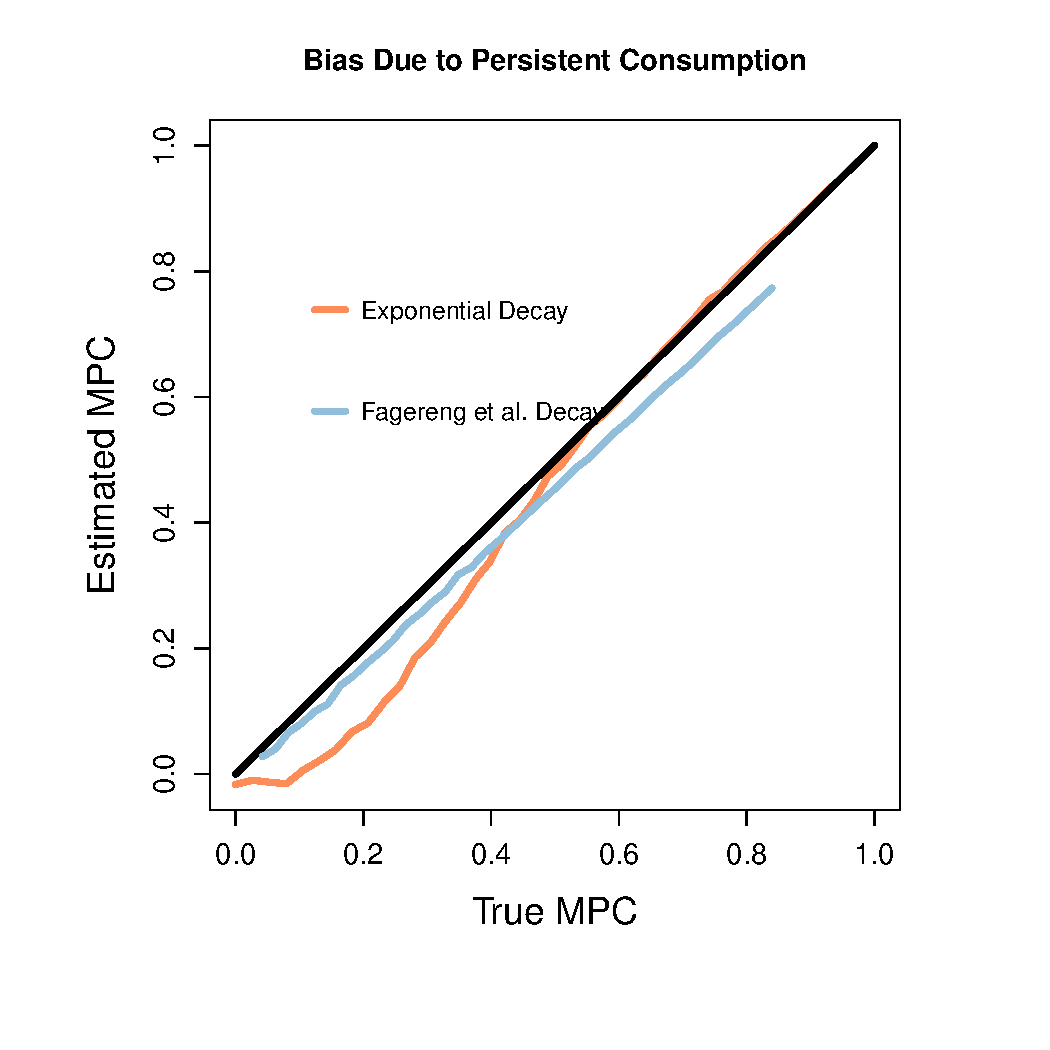
\includegraphics[scale=0.4]{\econtexRoot/Figures/DecayBias.pdf}
		\caption{Bias from Persistent Consumption}
		\label{fig:DecayBias}
	\end{centering}
\end{figure}

\subsection{Measurement Error} \label{Measurement_error}
Our identification comes from estimating $\mathrm{Var}(\Delta^N \bar{y})$ and $\mathrm{Cov}(\Delta^N \bar{c},\Delta^N \bar{y})$ using our observed data. For unbiased estimates of $\mathrm{Var}(\Delta^N \bar{y})$ we require no measurement error in our observed changes in labor income. For unbiased estimation of $\mathrm{Cov}(\Delta^N \bar{c},\Delta^N \bar{y})$ we only require (further to no measurement error in income growth) that the measurement error in expenditure growth is uncorrelated with labor income growth. As our expenditure is imputed from income and changes in assets, this is potentially more of a concern than would be the case in survey data in which questions about consumption are not directly linked to those on income. Below we examine potential sources of error in labor income and imputed consumption.

\subsubsection{Labor Income}
For most workers labor income is well measured. Third party reporting, along with a high level of trust in government institutions, means that underreporting is likely very low. The black eocnomy in Denmark is small, and to the extent that any growth in unreported income is uncorrelated with growth in reported income this will not bias our estimates.\footnote{Such income may show up as a change in net wealth and hence expenditure, but measurement error in the change in expenditure uncorrelated with the change in labor income will not bias our MPX estimates.} In contrast to survey data, in which measurement error in income is likely to downward bias transitory MPX estimates, this is of very little concern in our data.

\subsubsection{Imputed Expenditure}
Expenditure is calculated as the residual of total household income (including interest and dividends) after pension contributions and the change in net wealth have been deducted. For households with simple financial lives (which we believe fits most of the Danish population), this should work well. There are a few scenarios which merit further investigation.
\begin{itemize}
	\item \textbf{Stock Market Capital Gains:} Only 10\% of Danish households directly own stocks or mutual funds.\footnote{In our calculation we directly observe flows in and out of pension accounts, so these can be treated as off balance sheet in which capital gains do not affect our expenditure caluclation.} In appendix \ref{robustness} we show the qualitative patterns we observe are unchanged even when we completely remove these households from the sample. For households that do own stocks, we assume the return they receive is equal to a diversified portfolio of Danish stocks. Given that different households will have their own idiosyncratic portfolios, this methodology will results in significant measurement error. \cite{baker_measurement_2018} show not only that the size of this measurement error is correlated with income and wealth, but also with the business cycle. Furthermore, \cite{fagereng_persistence_2016} show that some groups of investors consistently outperform the market, which would lead us to consistently underestimate their expenditure. Our concern, however, is that the \textit{change} in measurement error of expenditure be correlated with the \textit{change} in labor income. Consistently underestimating expenditure by the same amount is therefore not a problem for us. Furthermore, as we have removed all aggregate effects from the labor income residuals that we use in estimation, any measurement error correlated with the business cycle will be uncorrelated with our measure of changes in labor income. We see two potential ways in which mis-measuring stock returns may bias our results. First, if households are significantly invested in the stock of the firm they work for, likely only to be the case for high level management. Second, to the extent that households invest their labor income gains halfway through the year, we will underestimate expenditure for those whose income increases, and overestimate it for those whose income decreases. This would lead us to underestimate the MPX. The size of this bias is limited by the size of excess expected returns, so our MPX estimate will be biased by no more than a few percentage points.
	\item \textbf{Family and Friends Transfers:} If a household receives a transfer of money from their parents, for example, imputed expenditure will be lower than true expenditure by this amount. Large transfers typically occur upon death of a parent, which is likely uncorrelated with the household head's labor income, or when purchasing a house, years during which we have already excluded in our sample. However, to the extent that friends and family actively insure each other's labor income, our MPX estimates will be upward biased.
	\item \textbf{Off Balance Sheet Assets:} A larger concern is that some forms of saving may be hidden off balance sheet. All Danish banks and brokers are required to report their clients' holdings, so off balance sheet assets are likely to be either off-shore, or non-financial assets. This would be a large concern if we were focused on the expenditure of the super wealthy 0.1\%, but is less so when dividing the population into quintiles or deciles as we have done. Our imputation method would interpret this saving as expenditure, so our estimate of the MPX would increase one-to-one for each percentage point of saving out of income shocks performed off balance sheet.
\end{itemize}

\subsection{RIP or HIP Income Process?} \label{rip_hip}
Our method makes strong assumptions on the income process, namely that there is no persistent idiosyncratic component to income growth and that the process contains a random walk. \cite{guvenen_empirical_2009} shows that it is empirically difficult to distinguish between a ``Restricted Income Profiles'' (RIP) like this and a ``Heterogenous Income Profile'' (HIP) income process, in which i) shocks to income are much less persistent (eg AR(1) with $\rho\approx 0.8$), and ii) households have a persistent idiosyncratic growth component. The reason the RIP and HIP processes are difficult to tell apart is that the two features (i) and (ii) act in opposite directions on the cross-section variance of income growth. The less persistent income shocks lead the cross-sectional income growth variance not to grow as fast as the HIP model, while the persistent idiosyncratic growth component leads the same variance to grow at a faster rate. The result is that the increase in variance of income growth over three to four years is approximately the same as the increase from four to five years.\footnote{See appendix \ref{rip_hip_appendix} that shows how the variance of income growth over N years grows with N.} To the extent that the consumption response to these semi-permanent shocks is similar to the the response to the idiosyncratic persistent growth component,\footnote{See \cite{guvenen_learning_2007} for an example of why this might be the case: if households do not know their own idiosyncratic growth ex-ante, a Bayesian learning process will be very slow, so households (at least initially) will react in similar ways to changes in income due to this persistent growth component as a true income shock.} our methodology will continue to provide reasonable estimates of the `permanent' MPX and the more familiar transitory MPX. Appendix \ref{rip_hip_appendix} has more detail on this point.

\subsection{Time Varying Risk} \label{time_varying_risk}
We have assumed that idiosyncratic risk remains constant over time. Given that our sample period covers the great recession, this may not be appropriate. In appendix \ref{time_varying_risk_appendix} we show how the variance of income growth has varied over time, peaking just after the crisis in 2010. In order to test how much this time varying risk might bias our results, we simulated data with $\phi=1$ and $\psi=0.5$, with permanent variance equal to estimates from the data and transitory variance varying in order to match the time varying income risk pattern observed in the data. When we ran this simulation we found estimates of $\phi$ and $\psi$ within 1\% of their true values.

\FloatBarrier

\section{Conclusion}
In this paper we have presented a new and robust method to measure the sensitivity of consumption to permanent and transitory income shocks for different groups of households. Our focus has been to use this method to test the microfoundations of heterogeneous agent models and quantify the importance of consumption heterogeneity for monetary policy. With administrative data from Denmark we have been able to dig into the distribution of MPC across a variety of dimensions in far more detail than has previously been possible. We find MPCs vary systematically and in ways that are important for monetary policy transmission, although the current generation of heterogeneous agent models struggle to fit the high sensitivity to income that we observe.

Our hope is that the method we present in this paper, or variants of it, can also be of use to economists in a variety of fields. More and more high quality micro data on consumption is becoming available, such as the administrative data used here, or the even more detailed transaction level data available from financial aggregators. If this continues, as we hope it will, methods such as ours will become even more valuable in bridging the gap between models and data.





\processdelayedfloats

\small
\bibliography{AllPapers}
\normalsize

\pagebreak
\appendix
\renewcommand\thefigure{\thesection.\arabic{figure}}  
\renewcommand\thetable{\thesection.\arabic{table}}  

\section*{Appendix}

\section{Identification with Time Aggregation}\label{sec:Identification}

\setcounter{figure}{0}   
\setcounter{table}{0} 
\input\econtexRoot/Appendices/Identification3.tex

%\input\econtexRoot/Appendices/Identification2.tex

\section{Sample Selection} \label{sample_selection}
\setcounter{figure}{0}   
\setcounter{table}{0} 
We choose to look at households whose head is between the ages of 30 and 55 in 2008. This is driven by the desire to remove households for who the assumption that most of the income growth is unexpected is not likely to be fulfilled. For the old and the young it is likely that individual households will have a lot of information about their income path that is not available to the econometrician (for example the year in which they plan to retire, or the fact that they are on a specific career track with set expectations of promotion and pay raises). We also want to remove households whose income volatility is increasing or decreasing sharply. Figures \ref{fig:VarianceByAge} and \ref{fig:MPXByAge} show how our estimates of both income variance and MPX vary with age. The dots represent the point estimate for each age while the lines are the centered moving averages over the five nearest age groups. The solid black line shows the total variance of income growth over 1 year. It should not be surprising that income growth for households with heads in their 20's is highly volatile. This volatility plateaus around the age of 35 and stays at a constant level until the point of retirement at which point it temporarily grows before falling to an even lower level. We can see that while both transitory and permanent shocks to income are high early in life, permanent income shocks are particularly large while individuals find their place in the workforce. From the age of 30 to 55 both transitory and permanent shocks are approximately the same size and remarkably stable. At retirement shocks to permanent income rise, not surprisingly as retirement itself will be seen in the model as a shock, even as transitory income variance declines.

As the model assumes the variance to permanent and transitory shocks is constant in the observed period, interpretation of the numbers outside of the 30-55 age group needs to be treated with care. However, the figure clearly shows that within this age group the assumption of constant variance appears to be a reasonable one.

The dotted black line shows the variance of $\Delta y$ assuming no persistence in the transitory component. The fact that this line is slightly above the empirical variance of $\Delta y$ is consistent with some persistence in the transitory component of income, justifying our decision to exclude growth over one and two years in our identification.

The level of both permanent and transitory shock variance for households aged 30 to 55 is approximately 0.0035, reflecting a standard deviation of 6\%. Estimates using US data are significantly higher, especially for the transitory shock variance (for example \cite{carroll_nature_1997} estimate 0.02 for permanent and 0.04 for transitory). This difference may be due to lower income inequality in Denmark, more progressive taxation and more generous unemployment insurance. The lower transitory variance will also be due to significantly reduced measurement error relative to the survey based US data. 
\begin{figure} 
	\begin{centering}
		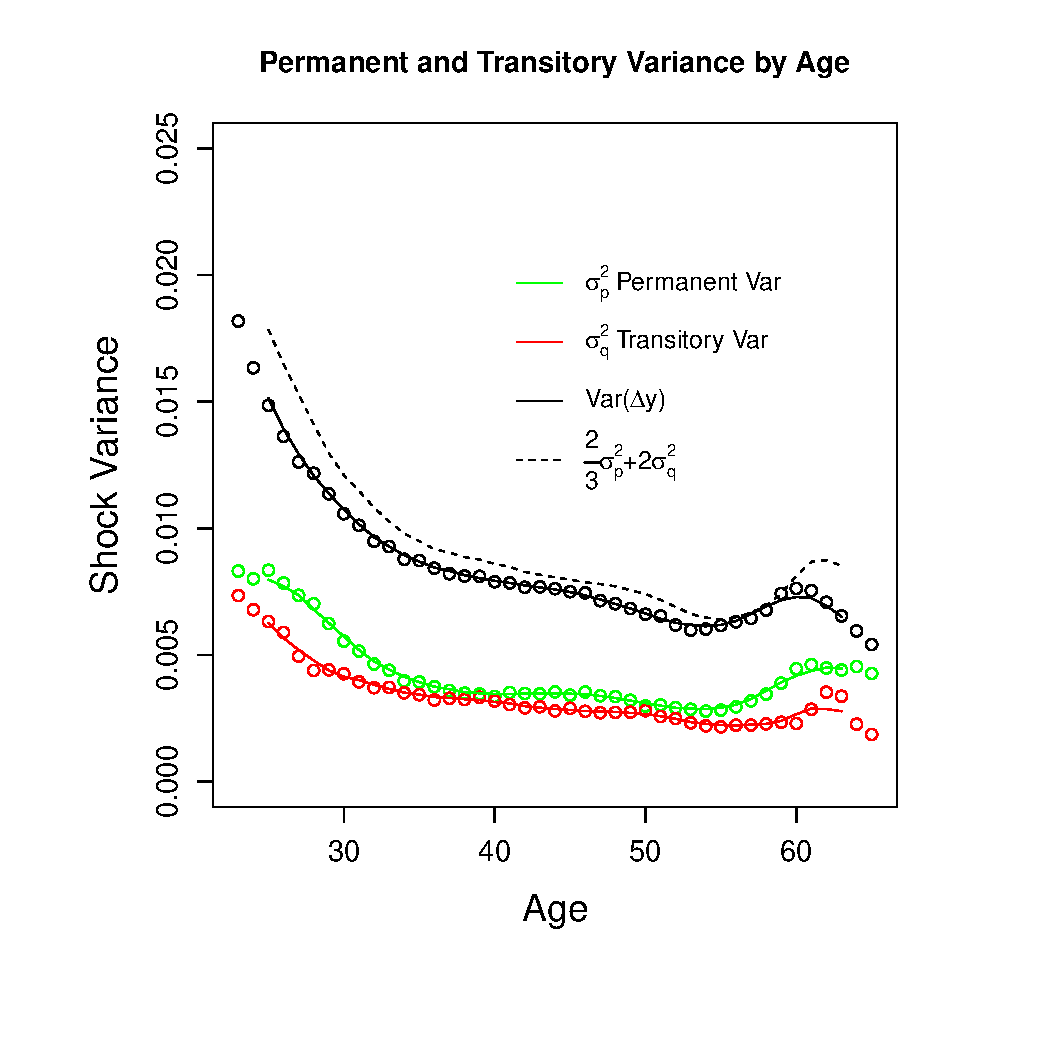
\includegraphics[scale=0.6]{\econtexRoot/Figures/VarianceByAge_level_lincome_head.pdf} 
		\caption{Permanent and Transitory Shock Variance by Age}
		\label{fig:VarianceByAge}
	\end{centering}
\end{figure}
\begin{figure} 
	\begin{centering}
		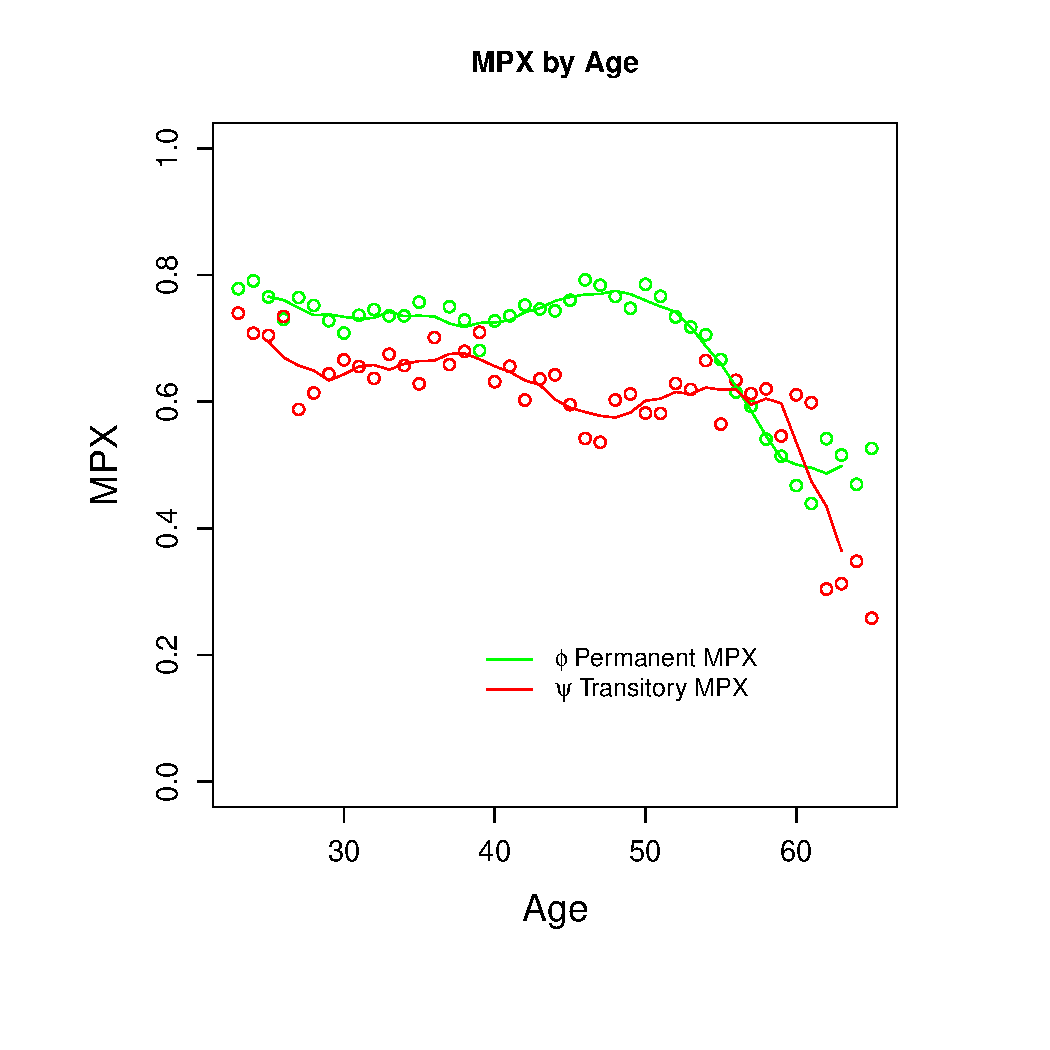
\includegraphics[scale=0.6]{\econtexRoot/Figures/MPXByAge_level_lincome_head.pdf} 
		\caption{MPX by Age}
		\label{fig:MPXByAge}
	\end{centering}
\end{figure}

\section{The Danish Mortgage Market} \label{mortgage_market}
\setcounter{figure}{0}   
\setcounter{table}{0} 
Mortgage loans in Denmark are issued by specialized mortgage banks, which fully finance loans by issuing bonds. Interest rates are directly determined by sales prices at the bond market. That is, borrowers only pay the bond market interest rate plus a supplementary fee for the mortgage bank. 
Most loans are issued as 20 or 30-year loans, and households can only obtain loans from mortgage banks of up to 80 per cent of the value at loan origination of properties used as permanent residences. The remaining (more insecure) part of the funding may be provided by commercial banks. The close link between loans and bonds, as well as fixed loan-to-value ratios, fast foreclosure procedures, full recourse, etc., mean that mortgage banks do not assume significant market risks. The status of Danish covered mortgage bonds as a safe asset class (AAA-rated by e.g. S\&P) imply that borrowers have access to very cheap real estate funding.

\begin{figure} 
	\begin{centering}
		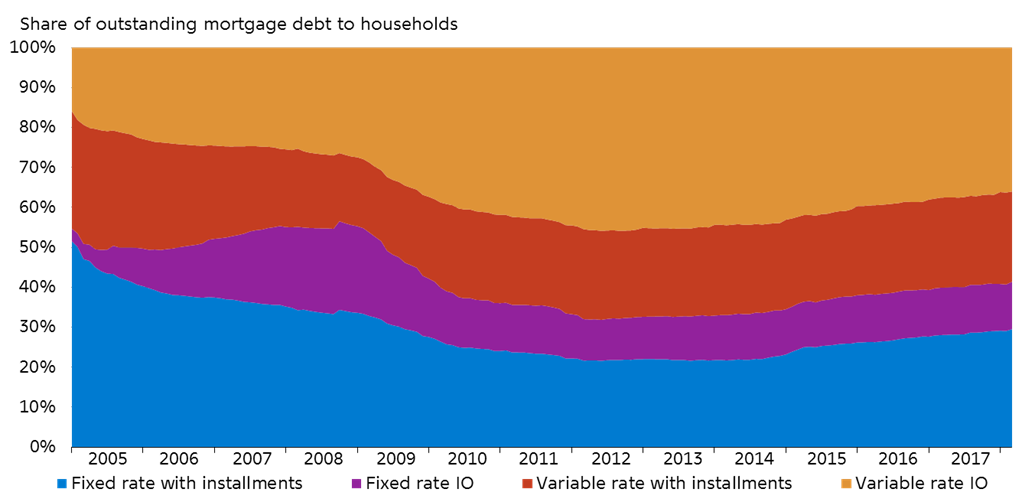
\includegraphics[scale=0.6]{\econtexRoot/Figures/mortgage_by_type.png} 
		\caption{Mortgage Debt by Type (all households)
		{\\ \emph{\footnotesize
	{Source: Danmarks Nationalbank}}
	}}
		\label{fig:mortgage_by_type}
	\end{centering}
\end{figure}

The Danish mortgage system has been functioning for two centuries, but significant liberalization has taken place over the past 20 years. Variable interest loans were (re-)introduced in 1996 while interest only loans were introduced in 2003. These new loan characteristics are by now very popular, see figure \ref{fig:mortgage_by_type}. In contrast to the US, where most mortgage debt is fixed rate, 40\% of mortgage debt in Denmark is variable rate, with interest fixation periods mostly between 6 months and 5 years. Fixed rate loans come with an option for early redemption. This implies that in practice, refinancing of fixed rate mortgages often take place, both when interest rates decrease and increase. The latter may be attractive because borrowers have the option to repay their loan by purchasing the corresponding amount of bonds. When interest rates increase, the bond value decreases, so the option to repay the loan by purchasing the corresponding amount of bonds in essence act as an equity insurance.  

\begin{figure} 
	\begin{centering}
		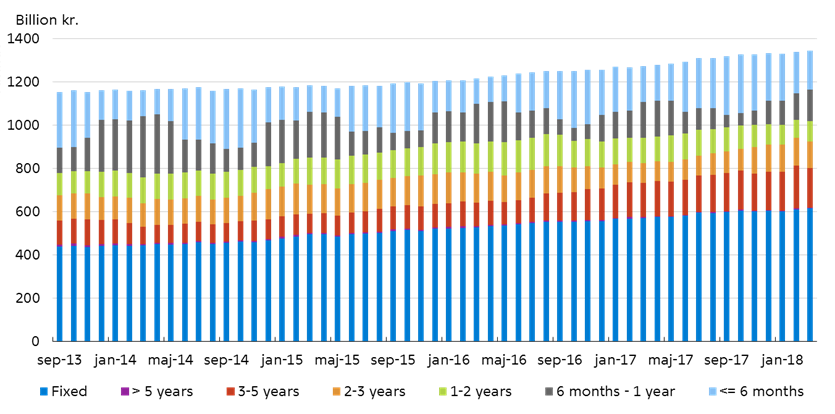
\includegraphics[scale=0.6]{\econtexRoot/Figures/mortgage_by_maturity.png} 
		\caption{Mortgage Debt by Maturity (all households excluding self-employed)
		{\\ \emph{\footnotesize
	{Source: Danmarks Nationalbank}}
	}}
		\label{fig:mortgage_by_maturity}
	\end{centering}
\end{figure}

Around one fourth of the total loan balance is due to have interest rates reset over a 12 month period (see figure \ref{fig:mortgage_by_maturity}). This figure only comprises loans that automatically will have a new interest rate, and not active decisions to refinance or extract equity. 

\section{Details on the calculation of NNP and URE}
\setcounter{figure}{0}   
\setcounter{table}{0} 
\label{URE_NNP_appendix}
The Net Nominal Position (NNP) and Unhedged Interest Rate Exposure (URE) for the various sectors in the Danish economy is calculated from our household level dataset as well as the financial accounts from the national accounts statistics. All calculations are based on average values over the years 2009-2015, deflated by the consumer price index. 

\subsection{NNP and URE for households}
The NNP for households is calculated as financial assets minus liabilities. As financial assets, we include bank deposits as well as the market value of securities (excluding shares). Liabilities include all debt to financial institutions (including credit card debt) as well as publicly administered student debt, tax debt and other debt to government bodies. These data are reported to the tax authorities by financial institutions on behalf of the households. 

URE is calculated as annual savings (i.e. after-tax income minus expenditure) plus maturing assets minus maturing liabilities. As maturing assets, we include all bank deposits, thereby assuming that they are floating rate. We assume a maturity of 5 years for securities held by households, and therefore include 20\% of the value of securities. Regarding liabilites, we assume that all bank debt is floating rate. According to the interest rate statistics collected by Danmarks Nationalbank since 2013, on average 95\% of bank debt from households is floating rate. Most of this is tied either to a market reference rate or to the Danmarks Nationalbank rate on certificates of deposit, with immediate adjustment. For mortgage debt, we have detailed information allowing us to calculate the stock of debt which is due to have interest rates reset over the coming 12 months. Voluntary refinancing of mortage loans, with or without extraction of additional equity, takes place to a large extent in Denmark. Our measure of maturing liabilities only includes the loans which contractually are due to have their interest rates reset, and we do not attempt to estimate the amount of additional refinancing. For remaining liabilities, which constitute very small amounts, we have no information regarding maturity, so we assume 5 years. 

\subsection{Other sectors}
NNP for the other sectors in the economy is obtained from the financial accounts statistics compiled by Danmarks Nationalbank. To most closely resemble the definition used in the household level data, we define NNP as net assets (i.e. assets minus liabilities) in the following categories: "Currency and deposits", "Securities other than shares", "Loans", and "Trade credits and other accounts receivable/payable". 

NNP for the whole economy should in principle sum to 0. However, the household level micro data on bank deposits that we have access to is exclusive of certain types of savings (specialized childrens savings accounts as well as some forms of pension savings accounts administered by banks) which are included in the financial accounts statistics. For the age group included in our sample, these types of accounts can be assumed to be largely illiquid. We therefore group those deposits (33 billion USD) together with the assets of pension funds (see table \ref{table:aggElas}).\footnote{In practice, this amount is calculated as a residual, which may also reflect other minor differences between the household level data and the national accounts statistics. For example, holdings of banknotes and coins are not observed in the micro data but allocated based on certain assumptions in the financial accounts. For our exercise, the impact of such other differences is likely to be very small.}

URE for non-households is also based on the financial accounts. We do not in the national accounts observe the maturity of different asset and liability classes. We hold household URE fixed at the values from the micro-level data and take advantage of the identity that total URE in the economy must be 0 to calibrate the maturity for the remaining sectors of the economy. This results in a maturity of assets and liabilities for non-households of 3.65 years.

\section{Persistent Consumption Response} \label{consumption_persistence_appendix}
\setcounter{figure}{0}   
\setcounter{table}{0} 
\subsection{Details on section \ref{Consumption_persistence} simulations}
For the simulations in section \ref{Consumption_persistence} we divided each year into 20 sub-intervals. Both permanent and transitory shocks occur each period, and the transitory shocks have no persistence. At an annual frequency the variance of permanent and transitory shocks are equal. Households spend their permanent income each period, along with their consumption response to the history of transitory shocks. For the exponential decay model this is:
\begin{align*}
c_t = p_t + (1-\rho)\sum_{n=0}^{\infty}\rho^n \varepsilon_{t-n}
\end{align*}
In \cite{fagereng_mpc_2016} the T year MPC is estimated as a function:
\begin{align*}
\text{MPC}_T = \theta_1 T^{\theta_2}
\end{align*}
Where $\theta_1$ controls the size of the response and $\theta_2$ the speed of decay. We vary $\theta_1$ and choose $\theta_2= 0.2142$ according to their estimate. In this model consumption in period $t$ (measured in sub-intervals) is:
\begin{align*}
c_t = p_t + \theta_1\sum_{n=0}^{\infty}\Big( (\frac{n+1}{20})^{\theta_2} -(\frac{n}{20})^{\theta_2} \Big)\varepsilon_{t-n}
\end{align*}
We then time-aggregate both income and consumption over each 20 sub-interval period, choose a sample of 13 years, and run our estimation procedure with $N=3,4,5$. The transitory MPC estimates are shown in figure \ref{fig:DecayBias}, the permanent estimates are shown here in figure \ref{fig:DecayBias_phi}. The bias in permanent estimates is small across the range of transitory MPCs.
\begin{figure} 
	\begin{centering}
		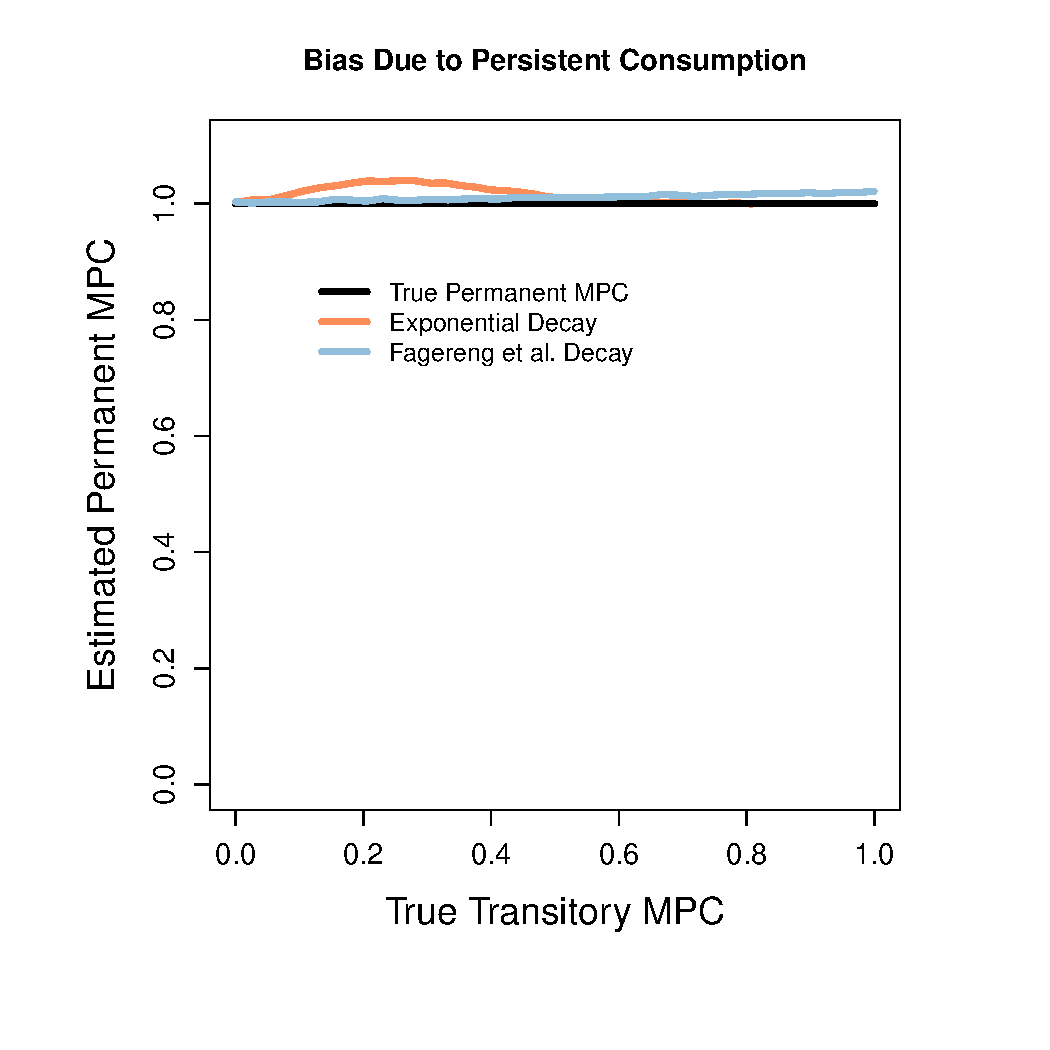
\includegraphics[scale=0.4]{\econtexRoot/Figures/DecayBias_phi.pdf}
		\caption{Bias from Persistent Consumption}
		\label{fig:DecayBias_phi}
	\end{centering}
\end{figure}

\subsection{Persistent Consumption in the Preference Shock Model}
Using a model we are able to calculate precisely the partial derivative of expenditure with respect to transitory income. To be comparable to the time period of our empirical MPX we take the mean MPX over 1,2,3 and 4 quarters:\footnote{Remember our empirical method measures the covariance of income with expenditure in the same calendar year. If the shock happens in the first quarter, then we will count expenditure over the next four quarters. If the shocks happens in the final quarter, then only one quarter of expenditure will be captured.}
\begin{align*}
\text{MPX}_{\text{model}} = 1 - \frac{1}{4}\sum_{i=1}^{4}(1-\text{MPX}_q)^i 
\end{align*}
where $\text{MPX}_q$ is the partial derivative in the quarterly model.
\begin{figure} 
	\begin{centering}
		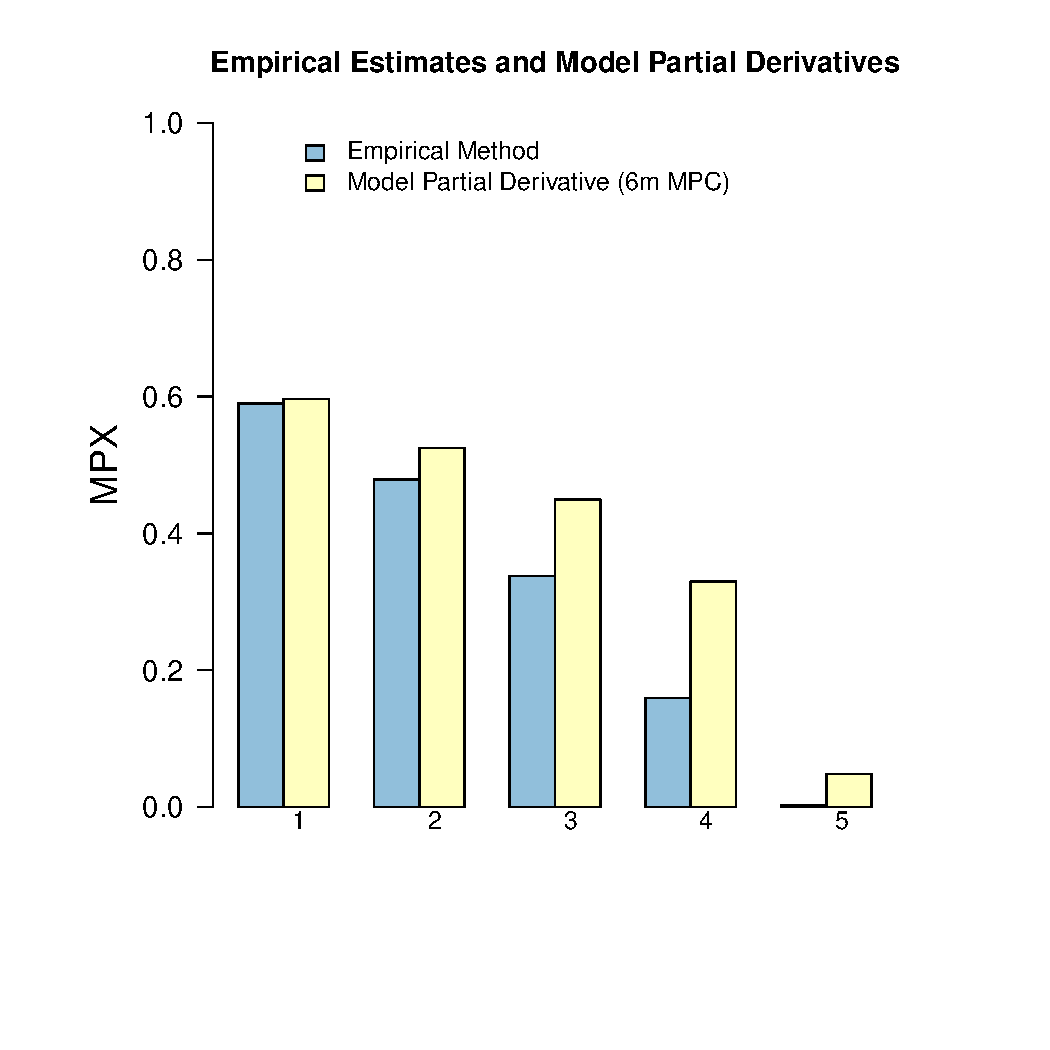
\includegraphics[scale=0.4]{\econtexRoot/Figures/MPC_accuracy.pdf}
		\caption{Empirical Method on Simulated Data versus Partial Derivative}
		\label{fig:MPC_accuracy}
	\end{centering}
\end{figure}

Figure \ref{fig:MPC_accuracy} shows how the empirical method performs on data simulated from the preference shock model of section \ref{model}. The method works well when the MPX is high, but overestimates the MPX when it is low. This is a direct result of the assumption that the consumption response to a transitory shocks decays within a two year period. The consumption response in the model is very close to the exponential decay model simulated above, so it is not surprising that the bias is large for low values of the MPX. As above, empirical evidence suggests that, even for households with low MPX, the initial decay of the consumption response occurs much faster than exponential decay would suggest.

\subsection{Estimates using different values of $N$}
\begin{center}
	\captionof{table}{$\psi$ Estimates using different $N$}
	\label{table:psi_estimates}
	\input ./Tables/Psi_array_empirical.tex
\end{center}
Table \ref{table:psi_estimates} shows the estimates of the transitory MPX that we recover from our estimation sample when we just use $N=n_1,n_2$ in our identification equations \ref{variance} and \ref{covariance}. Remember in our main results we used GMM with $N=3,4,5$ and we high circled $N=3,5$ to highlight where we get identification from in the paper. The purpose of this exercise is to show that the estimation results are not very sensitive to the values of $N$ chosen. This also provides more evidence that the assumption we made that the transitory consumption response lasts less than two years is not biasing our results significantly. In fact the results are not changed dramatically even when $N=1,2$, which suggests the majority of the transitory consumption response is very short lived.

\section{Labor Elasticity Model} \label{labor_elasticity_model}
\setcounter{figure}{0}   
\setcounter{table}{0} 
Here we detail the model and simulation results summarized in section \ref{labor_elasticity}. The model extends the standard incomplete markets model from section \ref{model}, incorporating both preference shocks, so that households have some years when their utility of consumption is greater than others, and labor elasticity, so that households can adjust their income based on the marginal utility of consumption. The household's problem is to maximize expected lifetime utility:
\begin{align*}
\mathbb{E}_t \sum_{n=t}^{\infty} \beta^n \Bigg(\mathcal{X}_n \frac{ \cLevBF_n^{1-\rho}}{1-\rho}-\frac{\lLevBF_n^{1+\frac{1}{\xi}}}{1+\frac{1}{\xi}} \Bigg)
\end{align*}
subject to the constraints:
\begin{align*}
\aLevBF_t = \mLevBF_t - \cLevBF_t \\
\bLevBF_t = R\aLevBF_t \\
\yLevBF_t =  l_t w_t \\
\lLevBF_t = l_t \pLevBF_t^{\frac{1-\rho}{1+\frac{1}{\xi}}}\\
w_t = \theta_t \pLevBF_t \\
\pLevBF_t = \Psi_t \pLevBF_{t-1} \\
\mLevBF_t = \bLevBF_t + \yLevBF_t
\end{align*}
The normalization of labor $(\lLevBF_t = l_t (\pLevBF_t^{\frac{1-\rho}{1+\frac{1}{\xi}}}))$ is set up to allow labor supply to move elastically with transitory income, but the long run supply of labor does not depend on permanent income (as observed in the consistency of hours worked over long time periods and across countries). The key additional features of this model are i) the preference shock factor and ii) the elasticity of labor.

Labor elasticity is controlled by the Frisch elasticity $\xi$. When the wage (relative to permanent income) increases by $x\%$, hours worked increase by $\xi\%$. We will examine values of the Frisch elasticity between 0 and 0.5 to cover the range of estimates from microeconomic studies.

\begin{center}
	\input\econtexRoot/Tables/beta_laborsupply50.tex	
	\input\econtexRoot/Tables/TranShk_laborsupply50.tex		\captionof{table}{Fitted discount factors and transitory shock standard deviation}
	\label{table:fitted_beta_and_transtd}
\end{center}

\begin{center}
	\input\econtexRoot/Tables/phi_laborsupply50.tex	
	\input\econtexRoot/Tables/c_std_laborsupply50.tex		\captionof{table}{Simulation estimates of $\phi$ and consumption growth standard deviation}
	\label{table:phi_laborsupply}
\end{center}

\begin{center}
	\input\econtexRoot/Tables/mpc_laborsupply50.tex
	\input\econtexRoot/Tables/psi_laborsupply50.tex		\captionof{table}{Simulation estimates of MPC and $\psi$}
	\label{table:psi_mpc_laborsupply}
\end{center}

In tables \ref{table:fitted_beta_and_transtd}, \ref{table:phi_laborsupply} and \ref{table:psi_mpc_laborsupply} we have varied the size of the Frisch elasticity and annualized preference shock. In each cell we have kept constant the overall annualized income growth variance and the median liquid asset to annual income ratio.\footnote{We calibrate to an annualized growth variance of 0.01 and a median liquid asset to annual income ratio of 0.5 to approximately match the upper quintile of the liquid wealth distribution.} To achieve this we vary the discount factor and the variance of transitory wage shocks.

Table \ref{table:fitted_beta_and_transtd} shows how the discount factor, $\beta$ and the annualized transitory shock standard deviation vary. As the size of the preference shocks increase, so does the precautionary motive for households. As we have fixed the median amount of precautionary savings, the discount factor drops slightly to compensate. The right hand panel shows the standard deviation of transitory shocks required to match the overall level of income growth variance goes down as labor supply elasticity increases. This is as expected - when the transitory wage is low households will work fewer hours. This amplifies the variance of the transitory income shock relative to the wage shock. The size of the preference shocks have little effect on the imputed size of the transitory shocks.

The left hand panel of table \ref{table:phi_laborsupply} shows the estimate of $\phi$ (the MPX out of permanent shocks) is close to 1 for variations of preference shocks and labor elasticities. This is unsurprising as labor does not respond to a change in permanent income. The right hand panel shows a very significant increase in the standard deviation of consumption growth as the size of the preference shocks increases. With no preference shocks, the standard deviation of consumption growth (0.05) is about half of the standard deviation of income (0.1). As the size of preference shocks increases, so does consumption growth variance, with the standard deviation growing to 0.26 for large preference shocks. This is still much smaller than 0.37, which comes directly from the data, although this high number from the data is likely to be contaminated with measurement error in assets. A further consideration is that much of the observed variance in expenditure growth will be due to durable items, such as home improvements and vehicles. We analyzed the effect of durables on our estimates in section \ref{durables}, but to the extent that these goods can be financed, our model with no borrowing may overestimate both the expenditure variance and the labor supply response to preference shocks.

Table \ref{table:psi_mpc_laborsupply} compares the actual mean MPC in the model with our empirical method for estimating the transitory expenditure elasticity. The left hand panel shows that both preference shocks and labor elasticity, often both missing in consumption models for simplicity, have quantitatively significant impacts on the implied marginal propensity to consume. Increasing the Frisch elasticity from 0 to 0.5 (the full range of micro-estimates) decreases the six month MPC from 6\% to just 3\%. This is because households now have an extra tool with which to insure against low consumption. When they receive a negative transitory shock to their wealth, they will consume less, which in turn will increase their marginal utility of consumption and induce them to work more hours. Therefore their actual income loss will be lower than the shock to their wealth and they will reduce their consumption by less than if they were unable to adjust their labor supply. In contrast, increasing the size of the preference shocks greatly increases the marginal propensity to consume. This is a result of the higher precautionary savings motive and consequently lower discount factor, even while median savings are unchanged.

The right hand panel of table \ref{table:psi_mpc_laborsupply} shows the effect of preference shocks and labor elasticity on our empirical estimates of $\psi$, the transitory MPX. The top row shows that our estimate is lower than the MPC (due to the fact that at these low levels of MPC, more than two years is required for the transitory effect to decay away). It does however follow the same pattern as the MPC and falls in magnitude as the ability of households to adjust labor supply increases. Similarly, going down the first row shows that the estimated MPX increases with the preference shock. However, the similarity to the MPX table ends when we increase \textit{both} labor elasticity \textit{and} the size of the preference shocks. Our estimate can grow large, up to a value of 0.25, when extreme values are chosen: a Frisch elasticity of 0.5 and a preference shock standard deviation of 0.4. This measured transitory MPX now bears little relation to the MPX (which is 0.08). Instead it is being driven by reverse causality, whereby preference shocks are driving consumption along with the decision to increase labor. The observed `shocks' to income are therefore highly correlated with consumption, but they are not causing the consumption dynamics exogenously.

This exercise suggests the bias due to reverse causality is likely to be small, but further investigation may be worthwhile.

\section{RIP or HIP Income Process?} \label{rip_hip_appendix}
\setcounter{figure}{0}   
\setcounter{table}{0} 
There has been a long-standing and unresolved quest in the literature to find a parsimonious representation of the labor income process. Two competing candidates are the Restricted Income Profile (RIP) and Heterogeneous Income Profile (HIP) processes. Both can be described by the equations:
\begin{align*}
	y_h^i = \beta^i h + z^i_h + \varepsilon^h_i\\
	z^i_h = \rho z^i_{h-1]} + \eta^h_i
\end{align*}
where $i$ indexes the worker and $h$ the years of experience. $\varepsilon^h_i$ represents a transitory shock to income, while $\eta^h_i$ is persistent. $\beta^i$ represents an idiosyncratic persistent growth factor.

In the RIP model, $\beta^i=0$ and $\rho$ is usually estimated to be very close to 1 (in this paper we assumed $\rho=1$). In the HIP model $\beta^i$ has a cross sectional variance $\sigma_{\beta}^2>0$ and $\rho$ is normally estimated to be significantly lower than 1, around 0.8. The reason these are difficult to tell apart is because the theory gives not strong indication in which model the cross-sectional variance of income growth over $N$ years should grow faster. In the RIP model with $\rho=1$, the cross-sectional variance of income growth increases linearly with $N$. In the RIP model with $\rho\approx 0.8$ the growth in the  cross-sectional variance of income growth will decrease due to the low $\rho$, but increase due to the idiosyncratic $\beta^i$.

Figure \ref{fig:increasing_diff} shows the empirical values for income growth variance and the covariance of income and expenditure growth over $N$ years. We have also plotted the fitted values for these statistics that are implied by our model when fitted to $N=3,4,5$ as we do in the paper. We see the empirical variance and covariance decline slightly below the model fitted line as $N$ becomes large. This fits with the finding that $\rho$ in the RIP model is usually slightly below 1.0, around 0.98 or 0.99. We also note that around the region where we achieve our identification ($N=3,4,5$), there is very little curvature in the empirical statistics and the increase in both variance and covariance is close to linear.

While this linearity around $N=3,4,5$ cannot help us distinguish between the RIP and HIP process, it does imply that our empirical methodology may be somewhat robust to misspecification along this dimension. If we assume that the expenditure response to a change in $z^i_h$ and to the increase from the persistent idiosyncratic growth are equal to $\phi$, and the response to a transitory shock is $\psi$, that is:
\begin{align*}
	\Delta^N c^i_h \approx \phi \Delta^N (\beta^i h + z^i_h) + \psi \Delta^N \varepsilon^h_i
\end{align*}
Then the fact that $\mathrm{Var}\big( \Delta^N (\beta^i h + z^i_h) \big)$ grows approximately linearly with $N$ means that our empirical method will correctly identify $\phi$ and $\psi$.

A full investigation of the implications of different income processes is beyond the scope of this paper but would be a very useful exercise for future research.
	
\begin{figure} 
	\begin{centering}
		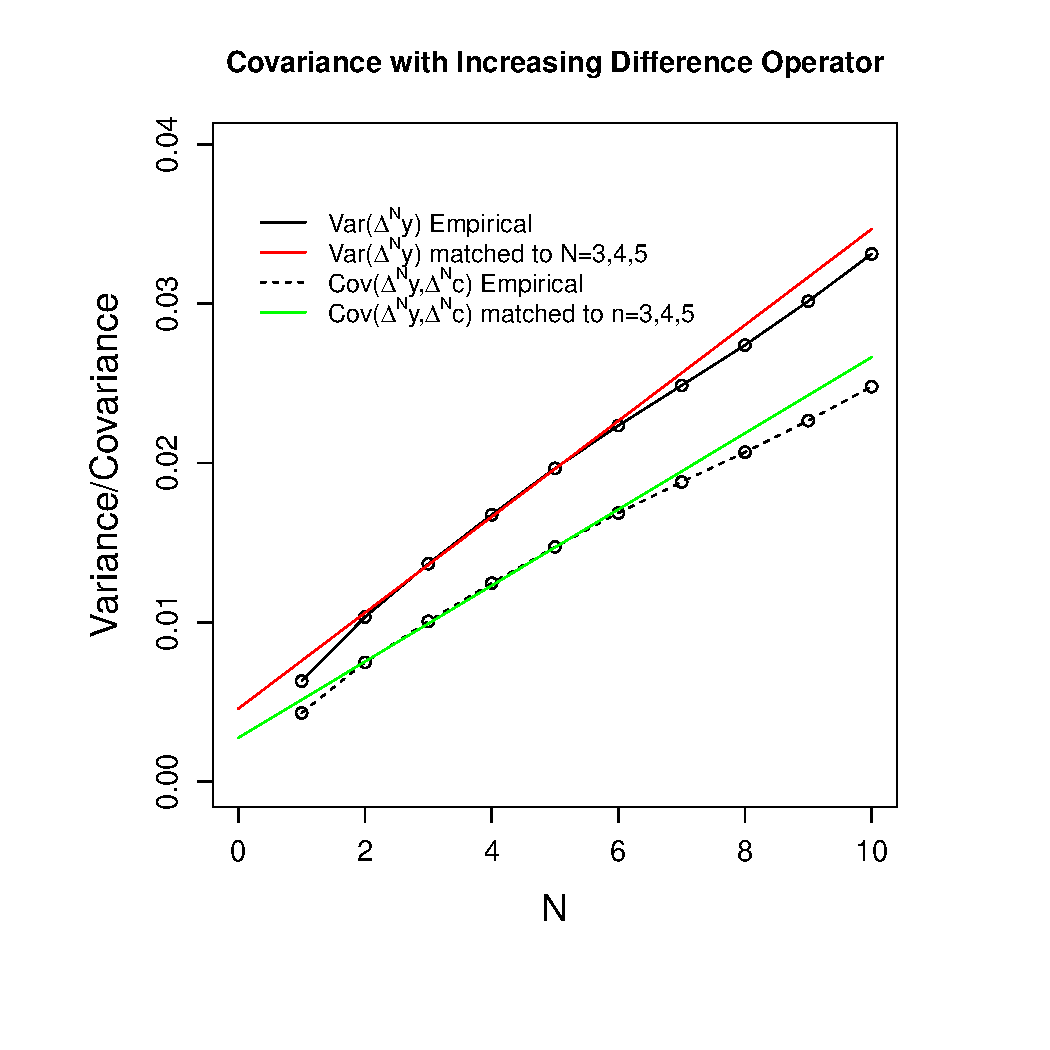
\includegraphics[scale=0.4]{\econtexRoot/Figures/IncreasingDiff_level_lincome_head.pdf}
		\caption{Variance and Covariance with Years of Growth}
		\label{fig:increasing_diff}
	\end{centering}
\end{figure}

\section{Time Varying Risk} \label{time_varying_risk_appendix}
\setcounter{figure}{0}   
\setcounter{table}{0} 
Figure \ref{fig:income_growth_std} shows how the standard deviation of income growth has changed over the sample period. From trough to peak the standard deviation increases approximately 10\%. In the simulation referred to in section \ref{time_varying_risk} we assume both transitory income and the transitory consumption response have no persistence. We divide each year into 20 subperiods, choose the variance of permanent shocks to be 0.003 and allow time varying transitory shocks to match the pattern in figure \ref{fig:income_growth_std}. We choose values of $\phi=1$ and $\psi=0.5$ and apply our estimation procedure (that assumes constant variance) to the simulated data. We recover estimated values of $\phi$ and $\psi$ to be 1.006 and 0.499 respectively.
\begin{figure} 
	\begin{centering}
		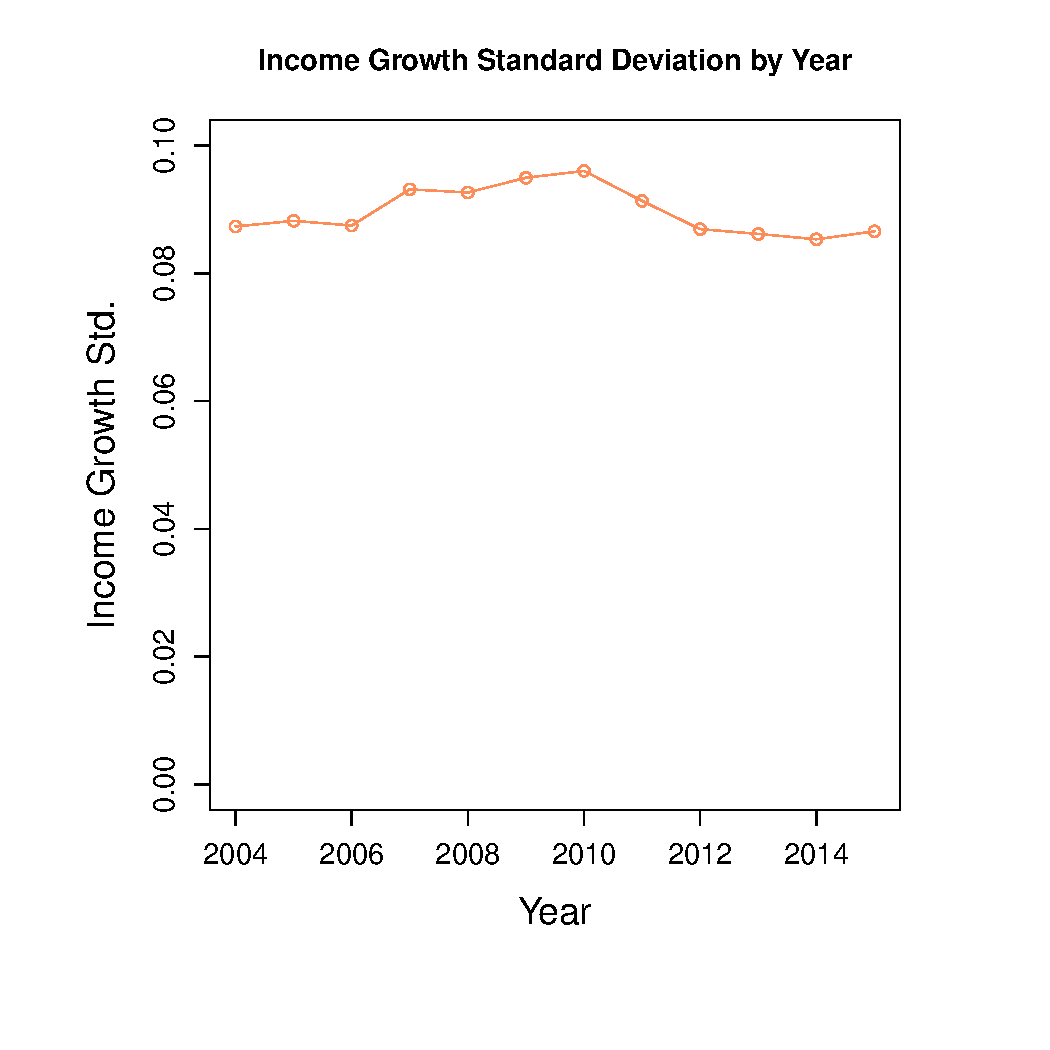
\includegraphics[scale=0.4]{\econtexRoot/Figures/IncomeGrowthStd.pdf}
		\caption{Standard Deviation of Income Growth}
		\label{fig:income_growth_std}
	\end{centering}
\end{figure}

\section{Robustness} \label{robustness}
As would be clear from the main text, we have made a number of choices regarding both data and variable definitions as well as more methodological issues. In a series of graphs this appendix presents a number of robustness checks aimed at assessing the extent to which our results are sensitive to the specific choices. 

We begin with a number of robustness checks regarding our imputed expenditure measure, which may suffer from measurement error. In figure \ref{fig:Robust_liquidURE}, we compare our baseline estimates of the MPX to estimates based on different sample selection procedures. First, we exclude all households that own stocks corresponding to more than 10,000 USD (10\% of households in our sample). Second, we do not remove households which have negative imputed expenditure. We remove those households in our baseline sample since negative expenditure is clearly not a good estimate of actual expenditure. However, for example in the event that negative expenditure arises because of classical measurement error, removal of negative estimates may be asymmetric and introduce an upward bias in average imputed expenditure. Third, to check that large outliers do not drive our results, we remove observations in the top and bottom 2.5\% in terms of level and change of income and expenditure. In the baseline calculations, we use only a 1\% cutoff. Our results are qualitatively unchanged when using these alternative approaches to take account of measurement error. In terms of magnitudes of the estimated MPX's, the largest difference to the baseline results seems to be found when we include negative expenditure estimates. As expected, this makes the largest difference among the wealthier households. The specification of outliers also matters somewhat for the point estimates of MPX in certain groups of households, but differences are not large. 

\begin{figure}
	\begin{centering}
		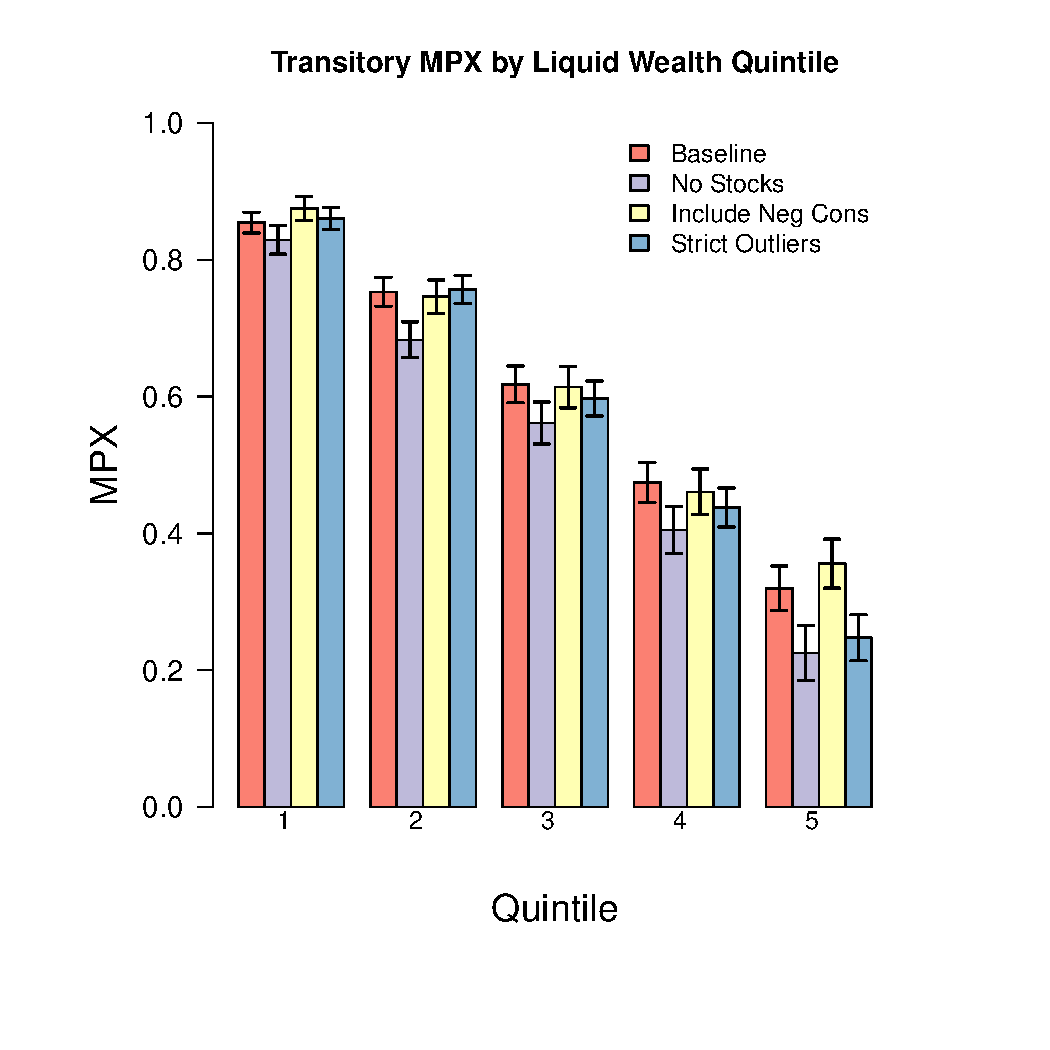
\includegraphics[scale=0.4]{\econtexRoot/Figures/Robust_tranMPX_liquidwealth.pdf}
		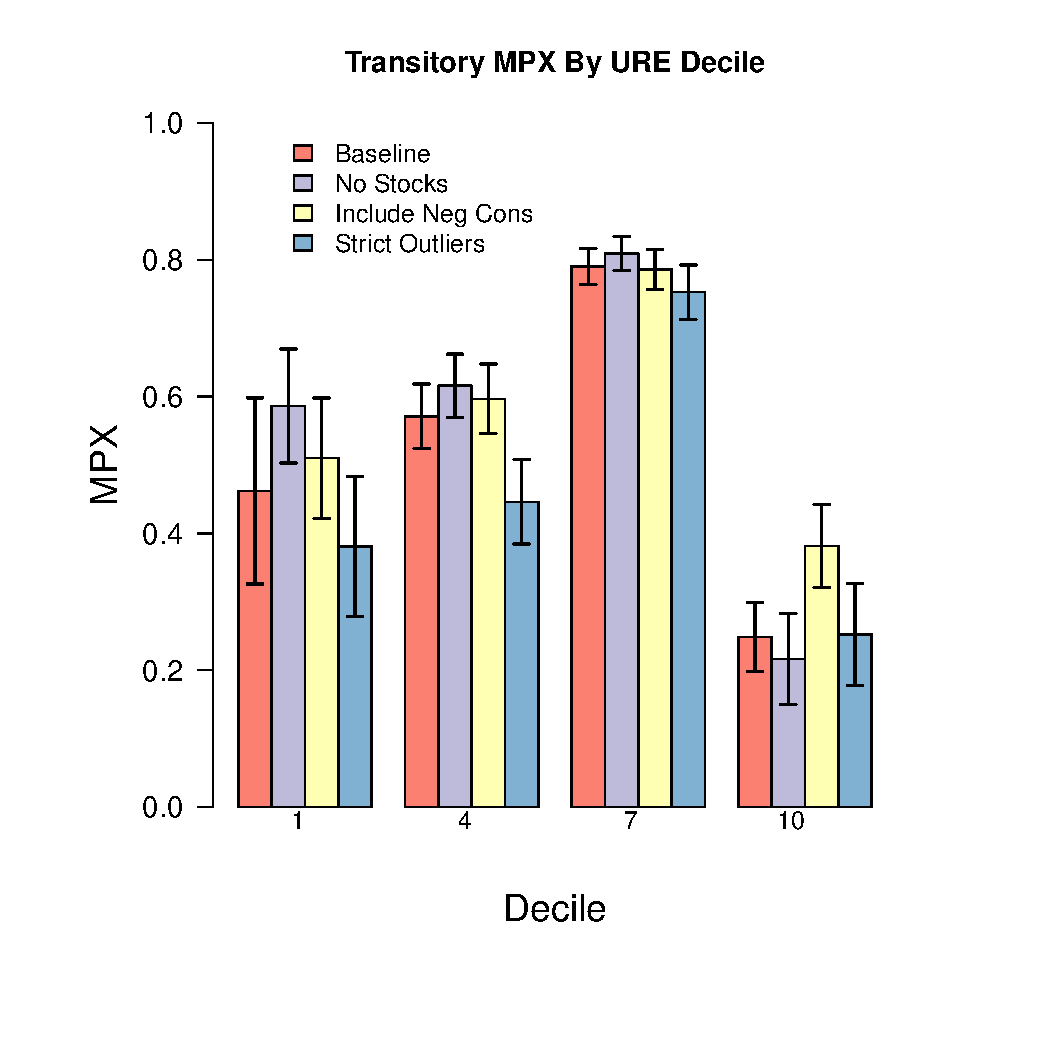
\includegraphics[scale=0.4]{\econtexRoot/Figures/Robust_tranMPX_URE.pdf}
		\caption{Robustness of Liquid Wealth and URE Distributions}
		\label{fig:Robust_liquidURE}
	\end{centering}
\end{figure}

Another robustness check consists of specifying consumption and income in logs rather than in levels. The fundamental difference is that the log specification yields an elasticity rather than an MPX. Hence, some difference between level and log results must be expected for households which only spend a fraction of their annual income (typically wealthier households). Indeed, as expected figure \ref{fig:Robust_Logs} demonstrates that results hold qualitatively when specifying income and expenditure in logs rather than in levels, whereas estimated elasticities are higher than the MPX's for the more wealthy households and those with high URE. Time varying income risk may also potentially contribute to differences between results based on levels and logs. However, as shown in section \ref{time_varying_risk} this is not likely to be important in our setting.  

\begin{figure} 
	\begin{centering}
		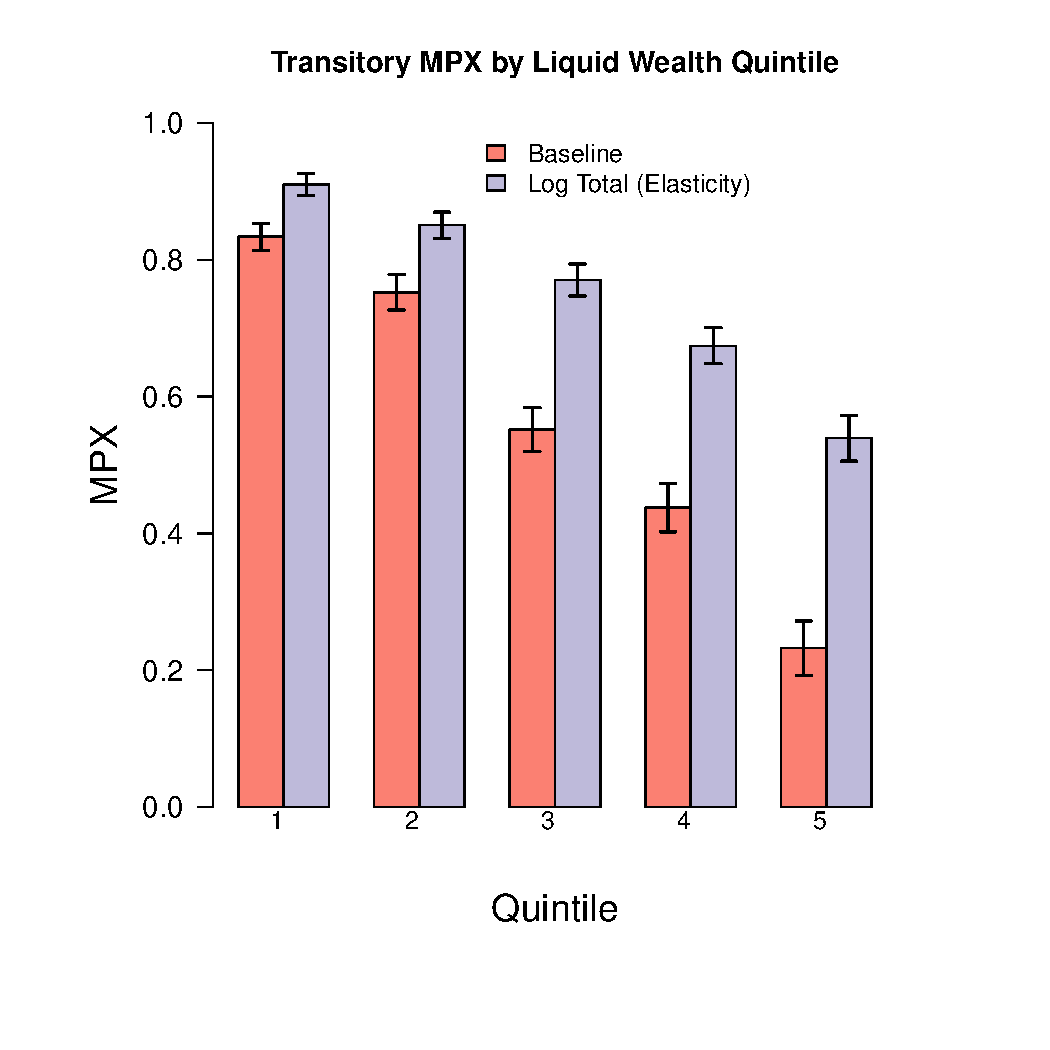
\includegraphics[scale=0.4]{\econtexRoot/Figures/Logs_tranMPX_liquidwealth.pdf}
		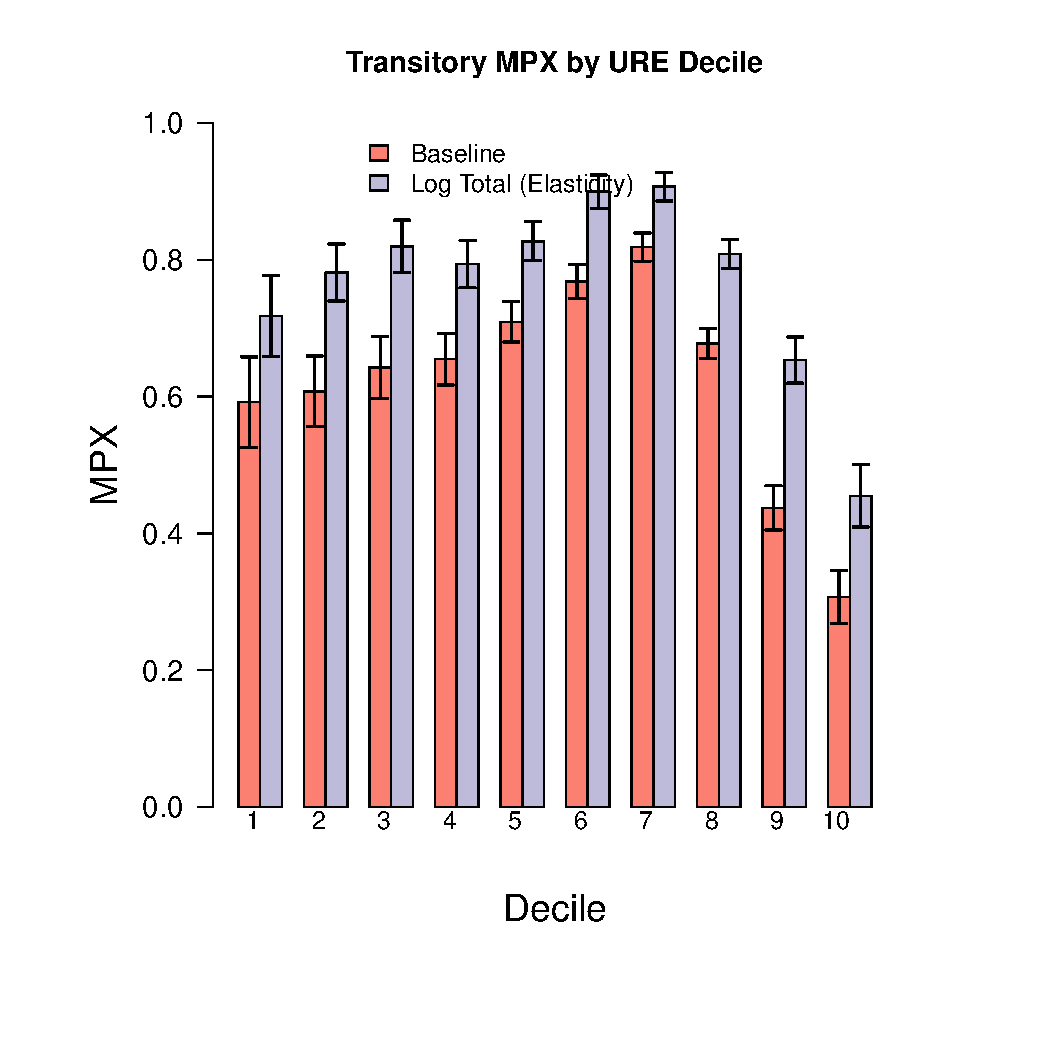
\includegraphics[scale=0.4]{\econtexRoot/Figures/Logs_tranMPX_URE.pdf}
		\caption{Results Using Log Income and Expenditure}
		\label{fig:Robust_Logs}
	\end{centering}
\end{figure}

As discussed in section \ref{income} we use labor income of the head of the household as our prime measure of income in line with previous literature. Various mechanisms, e.g. intra-household income insurance, may give rise to differences between results based on income of the head of household and total household income. However, figure \ref{fig:Robust_TotalvsHead} demonstrates that there is virtually no difference in our results between using total household income and only the household head's income. Appendix \ref{Insurance} briefly discusses the potential role that intra-household insurance may play, which we leave as an area for future research. 

\begin{figure} 
	\begin{centering}
		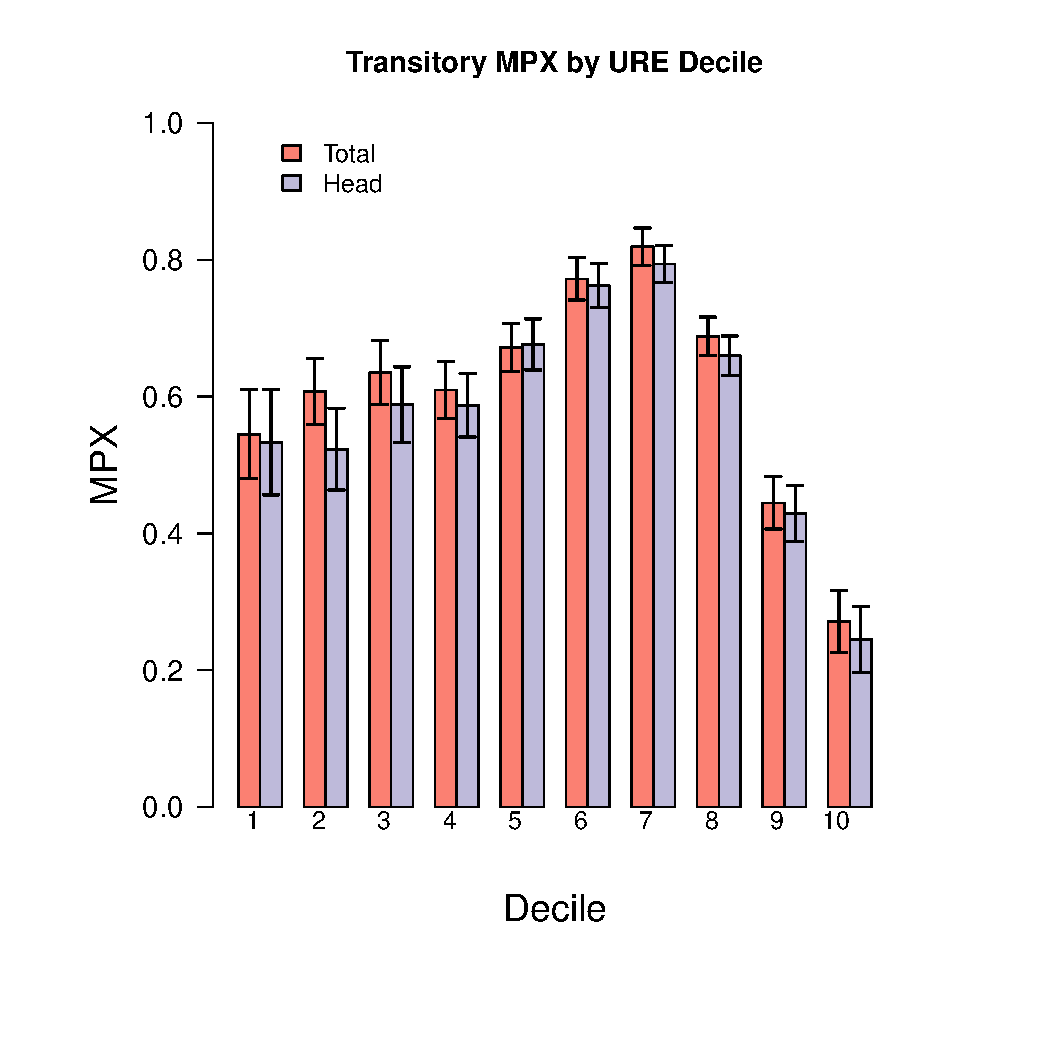
\includegraphics[scale=0.4]{\econtexRoot/Figures/total_tranMPX_URE.pdf}
		\caption{Results Using Total Labor Income and Head Labor Income}
		\label{fig:Robust_TotalvsHead}
	\end{centering}
\end{figure}

Finally, figure \ref{fig:MPXByLiquidWealth} shows the distribution of MPX by quintile of liquid wealth. It might be argued that the relevant level of liquid wealth is relative to income rather than in absolute terms. Figure \ref{fig:Robust_DivPerm} demonstrates that results based on quintiles of liquid wealth divided by permanent income are similar. Also, results (not shown here) where deciles are based on a broader definition of liquid wealth, i.e. including stock and bond holdings, are similar to our baseline results. 

\begin{figure} 
	\begin{centering}
		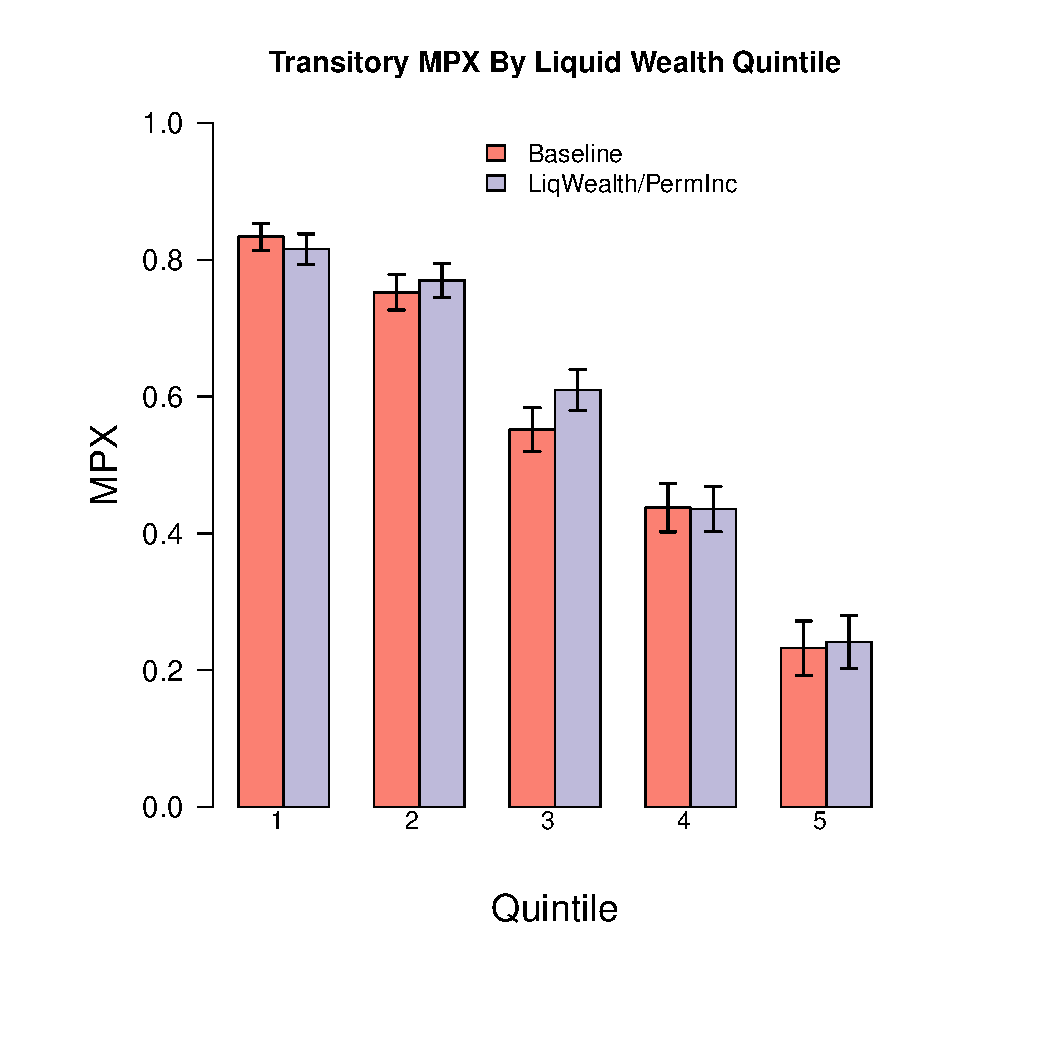
\includegraphics[scale=0.4]{\econtexRoot/Figures/DivPerm_tranMPX_liquidwealth.pdf}
		\caption{Results Using Quintiles of Liquid Wealth over Permanent Income vs Liquid Wealth}
		\label{fig:Robust_DivPerm}
	\end{centering}
\end{figure}


\section{Distribution of Permanent MPX by NNP, URE and Income} \label{PermMPXbyURENNP}
\setcounter{figure}{0}   
\setcounter{table}{0} 
Figure \ref{fig:MPCAuclert_perm} shows the distribution of both transitory and permanent MPX by NNP, URE and Income decile. The transitory numbers are a repeat of figure \ref{fig:MPCAuclert}.
\begin{figure} 
	\begin{centering}
		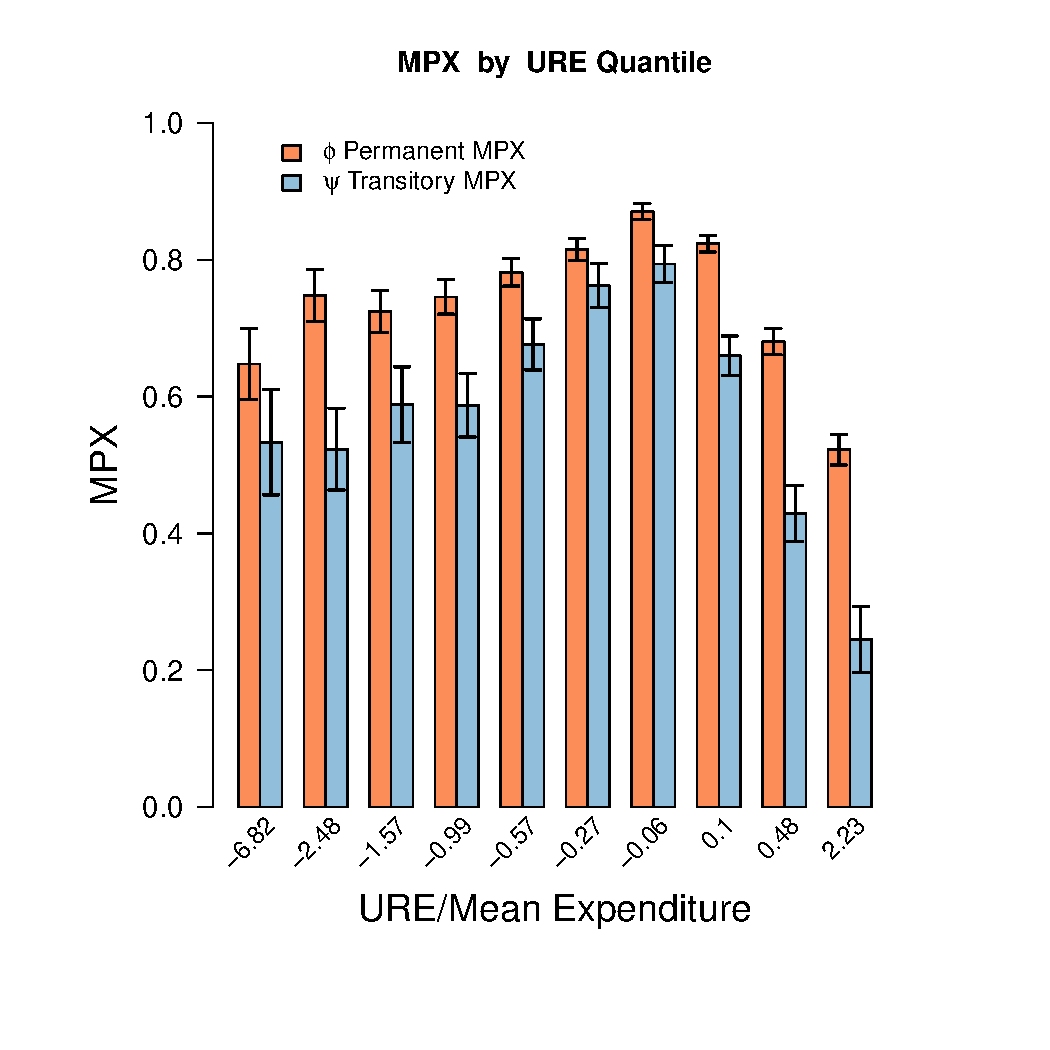
\includegraphics[scale=0.4]{\econtexRoot/Figures/MPXBypermURE_level_lincome_head.pdf}
		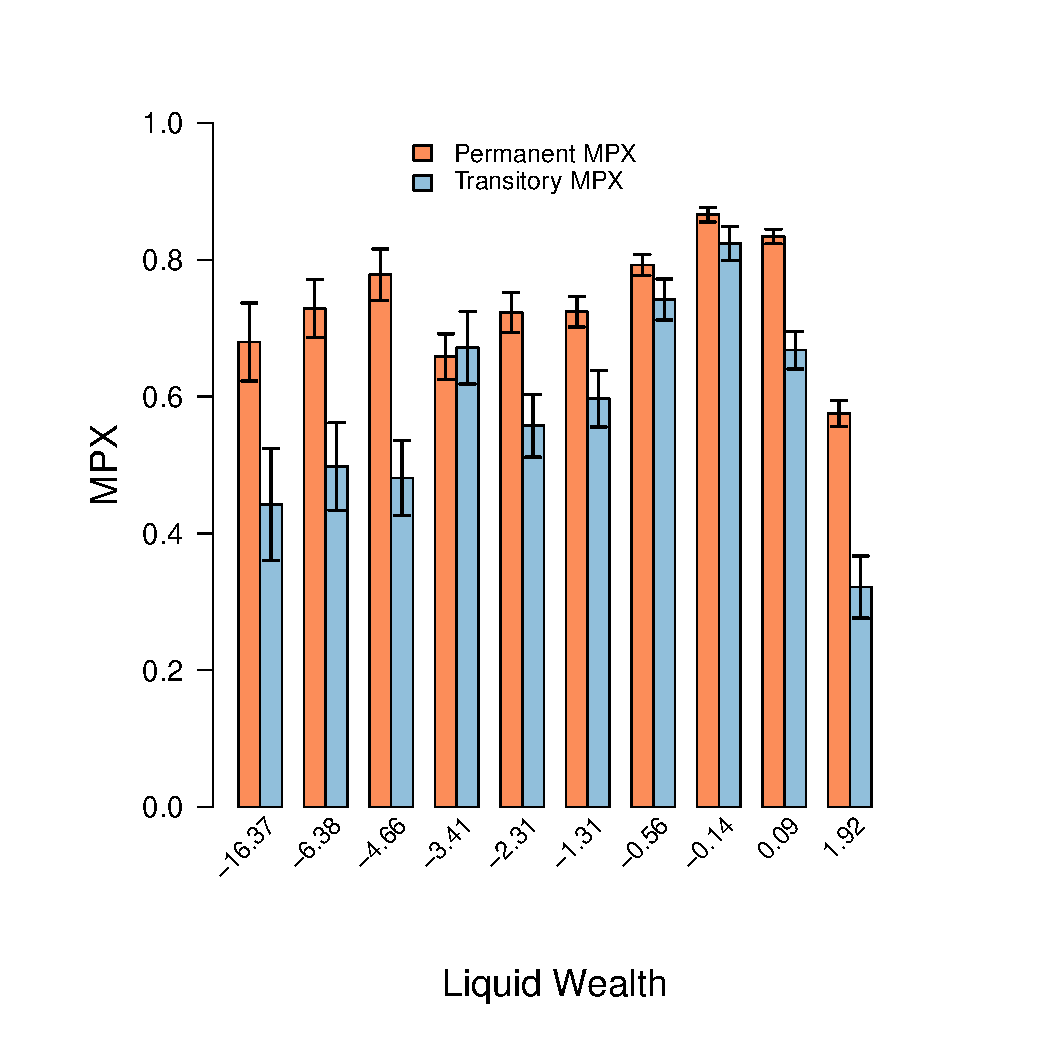
\includegraphics[scale=0.4]{\econtexRoot/Figures/MPXBypermNNP_level_lincome_head.pdf}
		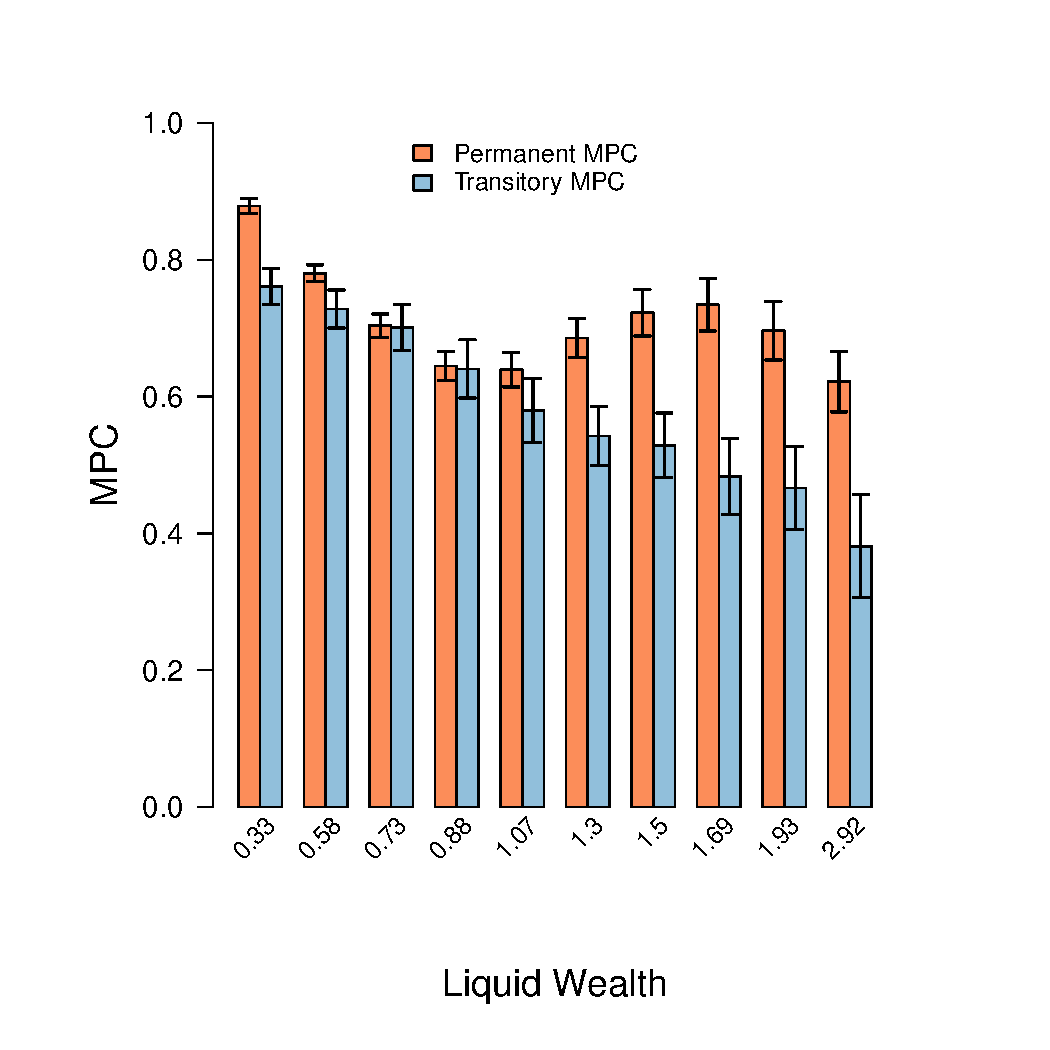
\includegraphics[scale=0.4]{\econtexRoot/Figures/MPXBypermIncome_level_lincome_head.pdf}
		\caption{MPX Distribution by URE, NNP and Income}
		\label{fig:MPCAuclert_perm}
	\end{centering}
\end{figure}

\section{Intra-household income insurance} \label{Insurance}
\setcounter{figure}{0}   
\setcounter{table}{0} 
As discussed in section \ref{income} we use labor income of the head of the household as our prime measure of income in line with previous literature. Figure \ref{fig:Robust_TotalvsHead} demonstrates that results based on total household income and income of the head of household are similar. However, MPX's from transitory shocks to the income of the spouse are lower than MPX's from shocks to total income, in particular for the less wealthy households, as demonstrated in figure \ref{fig:Robust_Spouse}. This indicates heterogeneity in the role that intra-household income insurance plays across different groups of households. We leave this interesting topic for future research. 


\begin{figure} 
	\begin{centering}
		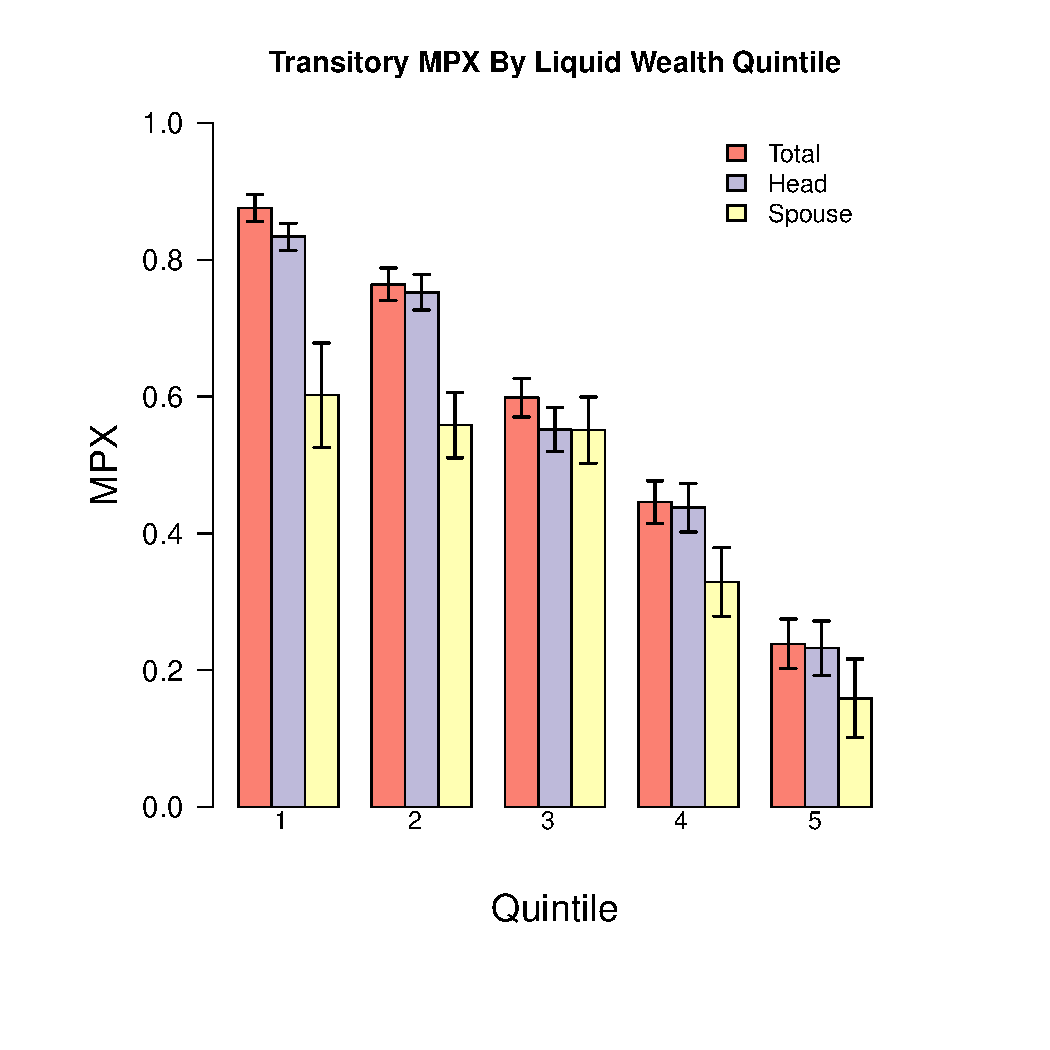
\includegraphics[scale=0.4]{\econtexRoot/Figures/Spouse_tranMPX_liquidwealth.pdf}
		\caption{Results Using Total, Head and Spouse Labor Income}
		\label{fig:Robust_Spouse}
	\end{centering}
\end{figure}

%\section{Simulation Results}\label{sec:Simulation}
%\input\econtexRoot/Appendices/Simulation.tex


%\AtEndDocument{
\includepdf[pages=-]{Backpage.pdf}}

\end{document}









